\documentclass[letterpaper,12pt]{article}
\usepackage{tabularx} % extra features for tabular environment
\usepackage{amsmath}  % improve math presentation
\usepackage{graphicx, subcaption} % takes care of graphic including machinery
\usepackage[margin=1in,letterpaper]{geometry} % decreases margins
\usepackage{xspace}
\usepackage{ANA-FTAG-2020-08-PAPER-defs}
\usepackage[style=numeric, sorting=none]{biblatex}
\addbibresource{ANA-FTAG-2020-08-PAPER.bib}
\addbibresource{Detector.bib}
\addbibresource{reconstruction.bib}
\addbibresource{bib/ATLAS.bib}
\addbibresource{bib/ATLAS-useful.bib}
\addbibresource{bib/PubNotes.bib}
\addbibresource{bib/ConfNotes.bib}
\addbibresource{bib/ATLAS-SUSY.bib}

\usepackage[final]{hyperref} % adds hyper links inside the generated pdf file
\usepackage[T1]{fontenc}
\usepackage{setspace}
\usepackage{float}
\usepackage{makeidx}
\usepackage{titlesec}
\usepackage{multirow}
\newcommand\bjetineq{\mathop{\mbox{$b$ $\rm{jet}$}}}
\newcommand\bjetunder{\mathop{\footnotesize{\mbox{$b$ $\rm{jet}$}}}\normalsize}
\newcommand\cjetineq{\mathop{\mbox{$c$ $\rm{jet}$}}}
\newcommand\cjetunder{\mathop{\footnotesize{\mbox{$c$ $\rm{jet}$}}}\normalsize}
\setcounter{secnumdepth}{4}
\newcommand{\specialcell}[2][c]{%
  \begin{tabular}[#1]{@{}c@{}}#2\end{tabular}}

\titleformat{\paragraph}
{\normalfont\normalsize\bfseries}{\theparagraph}{1em}{}
\titlespacing*{\paragraph}
{0pt}{3.25ex plus 1ex minus .2ex}{1.5ex plus .2ex}
\restylefloat*{figure}
\hypersetup{
	colorlinks=true,       % false: boxed links; true: colored links
	linkcolor=blue,        % color of internal links
	citecolor=blue,        % color of links to bibliography
	filecolor=magenta,     % color of file links
	urlcolor=blue         
}

%++++++++++++++++++++++++++++++++++++++++
\linespread{1.17}
\makeindex
\begin{document}

\title{Search for Higgs boson pair-production in the $bb\tau\tau$ final state using proton-proton collisions at $\sqrt{s}$ = 13 \TeV\ data with the ATLAS detector}%Fake Factors Calculation and Implementation in H$\rightarrow$ bb$\tau^+\tau^-$ analysis with MC16a/MC16d in Release 21 with the ATLAS detector
\author{ Zhiyuan Li}
\date{\today}
\maketitle
\begin{figure}[htp]
\centering
\includegraphics[width=.5\textwidth]{logo.png}
\vspace{3em}
\centering
\includegraphics[width=.45\textwidth]{ATLAS-Logo-Ref-RGB-H_1.jpg}
\end{figure}
\newpage

\tableofcontents{}
\printindex{}

\newpage
\section{Introduction}
\section{Theory and Motivation}
\subsection{The Standard Model and the Higgs boson}
\subsection{Beyond the Standard Model}
% \setcounter{secnumdepth}{4}

% \titleformat{\subsubsection}
% {\normalfont\normalsize\bfseries}{\theparagraph}{1em}{}
% \titlespacing*{\subsubsection}
% {0pt}{3.25ex plus 1ex minus .2ex}{1.5ex plus .2ex}
\chapter{The ATLAS experiment at the Large Hadron Collider}
\section{The Large Hadron Collider}

The Large Hadron Collider~\cite{Evans:2008zzb} is the world's 
largest and most powerful particle accelerator. 
It started operation in 2008 and retains its crucial role in the many 
accelerators in the world.
The collider is located in a ring tunnel of 
circumference 26.7 km, which lies beneath the 
French-Swiss border near Geneva, with superconducting magnets 
along the tunnel to keep the particle beam in direction
and a large number of accelerating structures to boost the 
beam to the desired energy.
Inside the tunnel, \textit{bunches} of up to $1.15 \times 10^{11}$ protons
travelling at close to the speed of light in opposite direction 
are collided 40~million times per second at four cross points,
around which are positioned four main detetors: 
ATLAS (A Toroidal LHC ApparatuS)~\cite{PERF-2007-01}, 
CMS~\cite{CMS-2008xjf} (Compact Muon Solenoid), ALICE (A Large Ion Collider Experiment) 
\cite{ALICE-2008ngc} and LHCb (b stands for beauty)~\cite{LHCb-2008vvz}.

% All the controls for the accelerator, its services and technical infrastructure 
% are located at the CERN Control Centre. 
% From here, the beams inside the LHC are made to collide 
% at four locations around the accelerator ring, 
% corresponding to the positions of four particle 
% detectors.

% two beams of particles travelling at close 
% to the speed of light 
% in opposite direction are made to collide. 


% Thousands of magnets are used to direct the beams 
% along the beam pipe, either to bend the beams or
% to focus them. The particles are so small that 
% making them collide is akin to firing two needles 
% 10 kilometers apart and getting them to meet halfway. 




	
\subsection{The LHC Accelerator Complex}

The proton beams colliding in the LHC are designed to carry energy 
of the order of a few TeV. To reach such high energy, a series of 
acceleration is required for the beams before entering the LHC ring. 
The protons are supplied by the injector chain Linac 2 — Proton Synchrotron 
Booster (PSB) — Proton Synchrotron (PS) — Super Proton Synchrotron (SPS), 
as shown in Figure~\ref{fig:accelerator_complex}.

\begin{figure}[bht]
	\begin{centering}	
	\includegraphics[width=.9\textwidth]{Detector_plots/accelerator_complex_smaller.png}
	\caption{The LHC is the last ring (dark blue line) in a complex chain of 
	particle accelerators. The smaller machines are used in a chain to help boost 
	the particles to their final energies and provide beams to a whole set of smaller experiments.
		}
	\label{fig:accelerator_complex}
	\end{centering}
\end{figure}

The protons are produced by stripping off the electrons from hydrogen gas
in an electric field. Linac 2, the first accelerator in the chain, 
is a linear accelerator which accelerates the protons to an energy of 50~MeV. 
They then enter the PSB, which accelerates the protons to 1.4~GeV, followed by 
the PS, where they reach 25~GeV. The series of radio frequency cavities in 
the PS splits the beam into discrete bunches of protons of 25 ns spacing. 
These bunches are then accelerated to 450~GeV in the SPS, from which they 
are finally injected into the beam pipes of the LHC. 
Each proton beam contains 2808 bunches, arranged in ``trains''
with 72 bunches each ``carriage'' of a gap of around 320 ns between each carriage. 
The beams are required to have well defined transverse and longitudinal emittance. 

The beam pipes are kept at ultra-high vacuum, a vacuum thinner than 
interstellar void, matianed for 24 km of low-temperature section and 3 km 
of room-temperature section. For the low temperature section, the vacuum is 
achieved by pumping in $9000$ m$^3$ of cryogenic gas, which later will be 
condensed and adhered to the surface of the beampipe. 
For the room temperature section, the vacuum 
is achieved by use of non-evaporable getter (NEG) that absorbs residue 
gas particles when heated. More residue is absorbed by an ion pumper. 

The beam pipes are installed in the existing tunnel that was constructed 
between 1984 and 1989 for the Large Electron-Positron Collider (LEP)~\cite{Myers:1991ym}, 
which lies between 45~m and 170~m below the surface on a plane inclined at 1.4\% sloping 
towards the Léman lake.
% Approximately 90\% of its length is in molasse rock, which has excellent 
% characteristics for this application, and 10\% is in limestone under the Jura mountain. 
% There are two transfer tunnels, each approxi-mately 2.5 km in length, linking the 
% LHC to the CERN accelerator complex that acts as injector. 
% These two beams are kept in separate beam pipes,
% cooled to $-271.3^\circ$C ($1.9$ K) with liquid 
% helium distributed by dedicated system, 
%  and ultra-high vacuum, 
There are advantages and disadvantages for a proton-proton collider,
compared to the electron-positron collider like LEP or proton-anti-proton collider.
% The proton-proton collider has advantages 
% and disadvantages compared 
For the LHC, two rings are needed to accommodate the two counter-rotating beams, 
unlike particle-antiparticle colliders that can have both beams sharing the same 
phase space in a single ring, and therefore sharing the same magnets, same radio 
frequency cavities, etc. However, LHC is able to achieve very high collision energy
which is not possible using electron-positron colliders, neither linear nor circular ones.
This is due to the fact that in a circular electron collider, synchrotron radiation lost is 
proportional to the Lorentz factor $\gamma = E/m$ to the power of four, where $E$ and $m$ are
the energy and mass of the particle, respectively. Since electrons are about
2000 times lighter than protons, synchrotron radiation lost is at the order of $10^{13}$
faster for electrons than for protons. For linear electron-positron collider, an extremely long
acceleration section is required with current technologies, which makes it an impractical option.
As for the proton-anti-proton collider, it would not be possible to achieve such 
high luminosity using anti-proton beams, since it is much more difficult 
to produce anti-protons than to produce protons. In addition, at high energies
the proton anti-proton collider starts losing one of its advantages of having higher cross section, 
which is due to the quark sea and anti-quarks in protons become more ``visible'' at high
energies (more details in the parton model section).
% In principle, since the mass of the proton is much larger than 
% the mass of the electron, the
% synchrotron radiation for the losses will be much smaller, and 
% the long straight sections designed to compensate the losses 
% (as designed for the LEP) can be reduced. 
% However these sections are kept 
% as the LEP has as a cost-effective solution, which avoids  
% re-excavating the tunnel. 
% The tunnel in the arcs has a finished internal diameter of 3.7~m. 

As explained above, two separate rings are required to accomodate the two beam pipes, while
the internal diameter of the tunnel is only about 3.8~m. It's technically challenging to 
install them in such small space. LHC therefore adopted the twin-bore magnet design~\cite{rossi2003lhc}, 
as shown in Figure~\ref{fig:double-bore-magnet}. It was first proposed by John Blewett at the Brookhaven 
laboratory in 1971 due to cost considerations~\cite{Blewett:1971zzb}, but in the case 
of the LHC the overriding reason for adopting this solution	is the lack of space in the tunnel. 
\begin{figure}[bht]
	\begin{centering}	
	\includegraphics[width=.7\textwidth]{Detector_plots/LHC-double-bore-magnet.jpg}
	\caption{ Double-bore magnet configuration of the LHC 
	superconducting magnets~\cite{rossi2003lhc}.}
	\label{fig:double-bore-magnet}
	\end{centering}
\end{figure}

\subsection{Luminosity and pileup}
% The aim of the LHC is to reveal the physics beyond
% the Standard Model with centre of mass collision energies of up to 14 TeV.
Luminosity is an important measure of a collider's performance.
It comes closely to the number of events generated per second, given by:
\[
	N = \mathcal{L}\sigma,
\]
where $\sigma$ is the scattering cross section 
for the event under study and $\mathcal{L}$ is the machine luminosity. 
For the cross-section, it is more common to use barn as the unit, 
where 1b~=~10$^{-28}$~m$^2$~=~10$^{-24}$~cm$^2$, 
since particle interactions usually have very small cross-sections. 
The machine luminosity depends on the beam parameters 
and can be written for a Gaussian beam distribution as:
\[
	\mathcal{L} = \frac{N_b^2 n_b f_{rev} \gamma_r}{4\pi \epsilon_n \beta*} F,
\]
where $N_b$~refers to the number of protons per bunch,
$n_b$~is number of bunches per beam,
$f_{rev}$~is the revolution frequency, 
$\gamma_r$~is the relativistic gamma factor, 
$\epsilon_r$~is the normalised transverse beam emittance, 
$\beta*$~is the beta function at the collision point which
describes the size of the beam, 
and	$F$ refers to the geometric luminosity reduction factor due to the 
crossing angle at the interaction point. 
While the instantaneous luminosity measures the rate of collisions (per unit cross-section), 
the total number of collisions (per unit cross-section) is measured by the integrated luminosity L, 
given by:
\[
	L = \int \mathcal{L} dt,
\]
which is the integral of the instantaneous luminosity over time.

The two general purpose experiments, ATLAS and CMS are
both aiming at a peak luminosity of $\mathcal{L}$ = $10^{34}$ cm$^2$s$^{-1}$ for proton proton collision,
which corresponds to about one billion $pp$ collisions per second. 
The instantaneous luminosity was much improved at real-time operations reaching about 
twice the nominal (from 2015 to 2018) thanks to the effort of the LHC experts. 

Another important parameter for the LHC experiments is the pileup, 
which is a measure of the number of inelastic $pp$ interactions that occur per bunch crossing. 
Higher pileup gives more luminosity (for a fixed number of bunches) 
but makes physics analysis more difficult due to the signals in the detector 
from the additional interactions. The distribution of the recorded luminosity over
the pileup is shown in Figure~\ref{fig:Run2_pileup} for operations from 2015 to 2018 (Run 2), 
where the <$\mu$> stands for the mean number of interactions per bunch crossing.
There are two main sources of pileup: in-time pileup and out-of-time pileup.
The former refers to the additional proton-proton collisions occuring in
the same bunch-crossing as the collision of interest. 
The later refers to the additional proton-proton collisions occuring
in bunch-crossings just before and after the collision of interest. 
% The out-of-time pileup is a challenge for the detector subsystems that 
% have sensitivity windows longer than
% 25 ns, the interval between bunch crossings.
%  It's a challenging task for the 
% trigger and reconstruction algorithms to achieve robustness under such high pileup 
% condition.
\begin{figure}[bht]
	\begin{centering}	
	\includegraphics[width=.6\textwidth]{Detector_plots/Run2_pileup.png}
	\caption{Shown is the luminosity-weighted distribution of the mean number of 
	interactions per crossing for the data collected by the ATLAS from 2015 to 2018. 
	All data recorded by ATLAS during stable beams is shown, and the integrated luminosity and 
	the mean $\mu$ value are given in the figure. 
		}
	\label{fig:Run2_pileup}
	\end{centering}
\end{figure}

% \subsection{Runs and results}


\subsection{Operation schedule}
\label{sec:Operation schedule}
The LHC operation and shutdown schedule is shown 
% in Figure~\ref{fig:LHC-longterm-schedule}
in Figure~\ref{fig:LHC-schedule-lumi}.
Following the downtime after an incident in one of the main dipole circuits 
during the first commissioning in 2008~\cite{lebrun2009report},
the operation restarted at lower beam energy to minimise the risk. 
Therefore, the first proton run (2010-2013)~\cite{alemany2013operation} was
carried out at 3.5–4 TeV per beam (centre of mass energy 7-8 TeV). 
Furthermore, a bunch spacing of 50 ns was used instead of the nominal 25 ns,
% This implied fewer bunches with larger intensity and hence a 
with peak luminosity of 0.8 $\times$ 10$^{34}$ cm$^{-2}$s$^{-1}$, 
% still smaller than
% the nominal 10$^{34}$ cm$^{-2}$s$^{-1}$ luminosity) 
and pileup larger than nominal. 
% \begin{figure}[bht]
% 	\begin{centering}	
% 	\includegraphics[width=.9\textwidth]{Detector_plots/LHC-longterm-schedule.png}
% 	\caption{Longer term LHC operation schedule.% [source: https://lhc-commissioning.web.cern.ch/schedule/LHC-long-term.htm]
% 		}
% 	\label{fig:LHC-longterm-schedule}
% 	\end{centering}
% \end{figure}

\begin{figure}[bht]
	\begin{centering}
	\includegraphics[width=.95\textwidth]{Detector_plots/LHC-schedule-lumi.jpg}
	\caption{LHC operation schedule and luminosity targets.  %[source:project HL-LHC, https://project-hl-lhc-industry.web.cern.ch/content/project-schedule ]
		}
	\label{fig:LHC-schedule-lumi}
	\end{centering}
\end{figure}
In Run 1, the LHC delivered about 30~\fb\ of proton data and important physics results,
most notably the discovery of the Higgs boson~\cite{HIGG-2012-27,HIGG-2012-28}.
Run 1 was followed by a long shutdown (LS1, 2013–2014)
with a large number of consolidation and upgrade activities~\cite{bordry2013first}. 	
The bus-bar splices between the superconducting magnets were improved, 
in order to make sure that the LHC could operate at higher energy 
without risk of repeating the 2008 incident. 

\begin{figure}[bht]
	\begin{centering}	
	\includegraphics[width=.6\textwidth]{Detector_plots/Run2_lumi.png}
	\caption{Cumulative luminosity versus time delivered to 
	ATLAS (green), recorded by ATLAS (yellow), and certified to be 
	good quality data (blue) during stable beams for $pp$ collisions 
	at 13 TeV centre-of-mass energy in Run 2. 
		}
	\label{fig:Run2_lumi}
	\end{centering}
\end{figure}

Run 2 (2016-2018) was carried out
at 6.5 TeV per beam (center of mass energy 13 TeV)~\cite{LHC-Run2-Operation}. 
As shown in Figure~\ref{fig:Run2_lumi}, out of the 156~\fb\ 
of data LHC has delivered at 13 TeV centre of mass energy, the ATLAS detector has recorded 
147~\fb\ and \lumi\ of data is certified to be good quality data.
The 156~\fb\ data accounts for the luminosity delivered from the start of 
stable beams until the LHC requests ATLAS to put the detector in a 
safe standby mode to allow a beam dump or beam studies. 
The recorded luminosity is slightly smaller than the delivered luminosity, due 
to the inefficiency of the Data Acquisition and the so called ``warm start'': 
when the stable beam flag is raised, 
the tracking detectors undergo a ramp of the high-voltage and, 
for the pixel system, turning on the pre-amplifiers. 
More details of the ATLAS detector can be found in the following sections. 
The recorded data is checked carefully to exclude possible hardware or software  issues. 
This is achieved by monitoring detector-level quantities 
and reconstructed collision event characteristics at key stages of the data processing chain.
This procedure led to high efficiency of good quality data: 95.6\%~\cite{aad2020atlas}.	



In this thesis the \lumi\ data recorded by the ATLAS detector of Run 2 is used.
The nominal bunch spacing of 25 ns was used, with slightly less bunches (2500) per beam.
The LHC experts have continually improved the running scenario to increase the luminosity,
and during Run 2 the luminosity surpassed the designed luminosity by a factor of 2. 
As well as improving the instantaneous luminosity, the availability of the machine
was dramatically improved during Run 2 which is an important factor enabling the high efficiency 
of good quality data as mentioned above.
During Run 2, the machine was providing physics collisions during 50\% of 
the allocated physics time, which is very impressive for a super conducting collider. 

The operation of CERN’s accelerators is subject to scheduled shutdowns 
to allow important repair and upgrade work to take place. 
The present shutdown, LS2, is devoted to preparations for Run 3 of the LHC, 
which will have an integrated luminosity equal to the two previous runs combined, 
and for the High-Luminosity LHC (HL-LHC), 
the successor to the LHC, which will begin operation at the end of 2027,
and eventually generate 10 times the integrated luminosity of
all Run 1, 2 and 3 combined!

The LS2 schedule has had to be modified due to the COVID-19 pandemic, 
which the new schedule anticipates that the first test beams will 
circulate in the LHC 
at the end of September 2021, four months later than the date 
planned before the COVID-19 crisis, 
to give the LHC’s main experiments – ATLAS, CMS, ALICE and LHCb – 
time to prepare their own upgrade. 
Run 3 of the LHC will begin at the start of March 2022.
% No changes have been made to the schedule beyond 2022.
The third long shutdown (LS3) will begin at the 
start of 2025 and end in mid-2027. 
This is when the equipment for the HL-LHC and 
its experiments will be installed. 






\section{The ATLAS Detector}


ATLAS is one of the two general purpose detectors built for probing proton-proton 
collision. This detector represents the work of a large collaboration 
of several thousand physicists, engineers, technicians,
and students over a period of fifteen years of dedicated 
design, development, fabrication, and installation.
The overall layout of the detector is shown in Figure~\ref{fig:ATLAS_cut_away}~\cite{PERF-2007-01}.
It has the shape of a cylinder, 46~m long, 25~m in diameter, 
and sits in a cavern 100~m below ground. The ATLAS detector weighs 7000 tonnes, 
similar to the weight of the Eiffel Tower.
The detector itself is a many-layered instrument designed to detect some 
of most energetic particles ever created on earth. 
It consists of six different detecting subsystems wrapped concentrically 
in layers around the collision point of nearly 4$\pi$ solid angle coverage
to record the trajectory, momentum, and energy of particles, 
allowing them to be individually identified and measured. 
These six subsystems are 
the pixel detector~\cite{ATLAS-TDR-11}, 
the semiconductor tracker (SCT)~\cite{ATLAS-TDR-04}, 
the transition radiation tracker (TRT)~\cite{ATLAS-TDR-04},
the electromagnetic (EM) calorimeter~\cite{ATLAS-TDR-02}, 
the hadronic calorimeter~\cite{ATLAS-TDR-03}
and the muon spectrometer (MS)~\cite{ATLAS-TDR-10}.
The first three sub-detectors are collectively known as the inner detector (ID),
described in section~\ref{sec:inner detector}, and it is used for tracking charged particles. 
The electromagnetic and the hadronic calorimeter, described in section~\ref{sec:calorimeter},
are responsible for measuring the energies of the electromagnetic and hadronic particles respectively. 
The MS, described in section~\ref{sec:MS}, is a unique sub-detector used for measuring the 
momentum of muons leaving the calorimeters.

A huge magnet system bends the paths of the charged particles so that their 
momenta can be measured as precisely as possible.

\begin{figure}[bht]
\begin{centering}	
\includegraphics[width=1.0\textwidth]{Detector_plots/Cut-away-view-of-the-ATLAS-detector.png}
\caption{Cut-away view of the ATLAS detector. 
The dimensions of the detector are 25~m in
height and 44~m in length. The overall weight 
of the detector is approximately 7000 tonnes. The figure is taken from reference \cite{PERF-2007-01}.
	}
\label{fig:ATLAS_cut_away}
\end{centering}
\end{figure}

The high interaction rates, radiation doses, particle multiplicities 
and energies, as well as the requirements for precision measurements 
have set strigent standards on the design of the ATLAS detector. 
Therefore the ATLAS detector is designed to fufiled the following 
requirements:




\begin{itemize}
\item
Fast, radiation-resistant electronics and sensor elements 
and high detector granularity. This is due to the
 high frequency of collisions, high particle fluxes and 
 high radiation environment of the detector.
\item
Large acceptance in polar angle with almost full azimuthal angle coverage,
due to the geometry of the detector 
(more details in section~\ref{sec:detector coordinate}).
\item
Good energy resolution calorimetry, as required to 
enable accurate physical object reconstruction. 
The high resolution of energy can be obtained 
with very good electromagnetic calorimetry for 
electron and photon identification and measurements,
complemented by full-coverage hadronic calorimetry 
for accurate jet and missing transverse energy measurements.
\item  
Tracking of precision in the ID, as required to provide high momentum 
resolution and to allow the reconstruction of
secondary vertices to identify $b$-hadrons and $\tau$-leptons.
\item
Good muon identification and momentum resolution 
over a wide range of momenta and the ability 
to determine unambiguously the charge of high-\pt\ 
muons in the muon spectrometer.
\item
Trigger system with high efficiency on low \pt\  
objects with sufficient background rejection, 
which is a prerequisite to achieve an acceptable trigger rate 
for most physics processes of interest.
\end{itemize}


The main performance goals of the detector are 
listed in Table \ref{tab:ATLAS_performance}. 
\begin{table}[thb]
	\centering
	\small
	\setlength\tabcolsep{5pt} 
	\begin{tabular}{|l|l|l|l| }
	\hline
	\multirow{2}{*}{Detector component}&\multirow{2}{*}{Required resolution} & \multicolumn{2}{l|}{$\eta$ coverage} \\ \cline{3-4}
	
	  & & Measurement &  Trigger\\ 
	 \hline
	Tracking         &    $\sigma_{p_T}/p_T = 0.05\%\ p_T\bigoplus 1\% $        &  $\pm 2.5$  & None \\  
	\hline
	EM calorimetry      &  $\sigma_E/E = 10\%\ /E\bigoplus 0.7\% $       & $\pm 3.2$ &  $\pm 2.5$\\
	\hline
	Hadronic calorimetry  &        & &      \\
	% \hline
	\ \ barrel and end-cap &  $\sigma_E/E = 50\%/E\bigoplus 3\% $       & $\pm 3.2$ &  $\pm 3.2$\\
	\ \ forward   &  $\sigma_E/E = 100\%\ /E\bigoplus 10\% $       & $ 3.1 < |\eta | < 4.9 $ &  $3.1 < |\eta | < 4.9 $\\
	\hline
	Muon spectrometer  &    $\sigma_{p_T}/p_T = 10\%$ at \pt $=\ 1$ TeV        &  $\pm 2.7$  & $\pm 2.4$ \\  
	\hline
	\end{tabular}
	\vspace{0.2cm}
	\caption{General performance goals of the ATLAS detector. The units for energy of the particle, E
	and transverse momentum, \pt\ (detailed definition in section~\ref{sec:detector coordinate}) 
	are in GeV~\cite{PERF-2007-01}. Note that, for high-\pt\ muons,
	the muon-spectrometer performance is independent of the inner-detector system.}
	\label{tab:ATLAS_performance}
\end{table}



\subsection{Coordinate system}
\label{sec:detector coordinate}

The ATLAS coordinate system is a right-handed Cartesian system
with the nominal interaction point 
defined as the origin of the coordinate system,  
while the beam direction defines the $z$-axis and 
the $x$-$y$ plane is transverse to the beam direction.  
The positive $x$-axis is defined as pointing from 
the interaction point to the centre of the
LHC ring and the positive $y$-axis is defined as 
pointing upwards, as shown in Figure~\ref{fig:ATLAS_coordinate_system}. 

\begin{figure}[bht]
	\begin{centering}	
	\includegraphics[width=.75\textwidth]{Detector_plots/ATLAS coordinate system.png}
	\caption{Illustration of the coordinate system
	used at the ATLAS experiment in the geographical context of the LHC.
		}
	\label{fig:ATLAS_coordinate_system}
	\end{centering}
\end{figure}

The azimuthal angle $\phi$ 	is measured as usual around the beam axis, 
and the polar angle $\theta$ is the angle from the beam axis.  
In high energy physics, it's more common to use the 
pseudorapidity instead of the polar angle $\theta$, defined as:
\[
		\eta = -\ln\ \tan(\theta/2). 
\]
In the case of highly relativistic particles
(which is the comman case in high energy physics), 
the pseudorapidity approaches the rapidity, 
\[ 
	y=1/2\ln[(E+p_z)/(E-p_z)], 
\]
where $E$ is the energy of the particle, $m$ is its mass 
and $p_z$ is the momentum along the $z$-axis.
There are two main reasons for using pseudorapidity 
rather than the polar angle $\theta$ nor the rapidity.
The reason for using pseudorapidity but not $\theta$ 
is that the rapidity is invariant
under Lorentz transformation, while capturing 
the characteristic of the particle direction of travel:
$y \rightarrow \pm \infty $ when the particle is  
travelling close to the beam pipe (positive for along the
beam pipe, negative for the opposite direction) and
$y \rightarrow 0$ when $p_z$ is small.
The reason for using pseudorapidity but not rapidity
is that due to the limited angle coverage of the detector, 
it's usually hard to determine the total energy and the momentum 
along the $z$-axis, especially when the direction of 
the particles are close to the beam pipe. 
While the pseudorapidity is determined only by
the polar angle, which is much easier and faster 
to compute. 
Another commonly used variable, transverse momentum \pt, 
is defined as the momentum of a particle transverse to the 
beam direction ($z$-direction):
\[ 
	\vec{p_T}= (p_x,p_y).
\]
The reason for using transverse momentum 
is that, because the partons that make up a proton share the momentum,
the initial longitudinal momentum is unknown;	
we do know, however, that the initial transverse momentum was zero. 
And hence we can look for the missing transverse momentum, defined
as 
\[ 
	E_T^{miss}=-\sum_i p_{T_i}  
\]
for visible particles $i$ (Confusingly $E_T^{miss}$ is commonly called 
missing transverse energy or MET. Missing transverse energy is equivalent 
to missing transverse momentum only if the missing particle(s) were massless.). 
Finnaly, the distance $\Delta R$ in the pseudorapidity-azimuthal angle 
space is defined as:
\[\Delta R = \sqrt{\Delta \eta^2+\Delta\phi^2},\]
where $R$ is the radial distance from the particle position to the interaction 
vertex.

\subsection{Magnets}


ATLAS has a unique hybrid system of four large superconducting 
magnets~\cite{ATLAS-TDR-06}. This magnetic system is 22~m in diameter and 26~m in length, 
with a stored energy of 1.6~GJ. Figure~\ref{fig:ATLAS_magnets_site} shows the real scale of
the magnets system compared to a person. 
Figure~\ref{fig:ATLAS_cut_away} shows the general layout, 
the four main layers of detetors and the four superconducting 
magnets which provide the magnetic
field over a volume of approximately 12000~m$^3$.



\begin{figure}[bht]
	\begin{centering}	
	\includegraphics[width=.8\textwidth]{Detector_plots/magnets.jpg}
	\caption{A picture showing the real size magnets compared to a person.}
	\label{fig:ATLAS_magnets_site}
	\end{centering}
\end{figure}




The spatial arrangement of the coil windings is shown in 
Figure~\ref{fig:ATLAS_magnets}. 
The ATLAS magnet system consists of two parts:
\begin{itemize}
	\item a solenoid, which is aligned on the beam axis and 
	provides a 2 T axial magnetic field in the $z$-direction
	for the ID. Becasue the magnet is located in front
	of the EM calorimeter, it is imperative to minimise possible interactions
	between the magnet and the particles being studied.
	This is achieved by embedding over 9 km of niobium-titanium 
	superconductor wires into strengthened, pure aluminum strips, 
	which is capable to provide such powerful magnetic field
	in just 4.5 cm thickness. 
	% while minimising the radiative thickness in front of the	barrel 
	% electromagnetic calorimeter;
	\item  A barrel toroid and two end-cap toroids, 
	which produce a	toroidal magnetic field of approximately 
	0.5 T and 1 T for the muon detectors in the central 
	and end-cap regions, respectively. 
	The barrel toroid generates the magnetic field in the central zone 
	of the muon spectrometer, along the tangential direction of 
	the circumferences centered on the $z$-axis ($\phi$ direction). 
	The end-cap toroids are two smaller toroids designed to 
	provide the magnetic field in the forward areas of 
	the muon spectrometer. 
	This magnet configuration provides a field is mostly orthogonal 
	to the muon trajectories. 
	
\end{itemize}		



\begin{figure}[bht]
	\begin{centering}	
	\includegraphics[width=.56\textwidth]{Detector_plots/ATLAS magnets.png}
	\caption{Geometry of magnet windings and
	tile calorimeter steel. Image taken from \cite{PERF-2007-01}.}
	\label{fig:ATLAS_magnets}
	\end{centering}
\end{figure}


\subsection{Inner detector}	
\label{sec:inner detector}
The inner detector (ID) is the closest sub-detector to the
beam line, designed to track the early trajectories of charged particles for
momentum calulations and locat their primary and secondary vertices with
extremely high precision. The ID is required to deal with large numbers of tracks
promptly, where 1000 particle collisions are taking place every 25 ns.  
The ID has full coverage in azimuthal angle $\phi$ and $|\eta|$ < 2.5 acceptance 
in pseudorapidity. As mentioned briefly above, it consists of three parts: 
the pixel detector and the insertable B-Layer (IBL)~\cite{ATLAS-TDR-19} (as one part),
the semiconductor tracker and the transition radiation
tracker. The layout of the ID is shown in figure~\ref{fig:inner_detector},
with a charge track (in red) traversing the sensors and structural elements. 
\begin{figure}[bht]
	\begin{centering}	
	\includegraphics[width=.85\textwidth]{Detector_plots/Inner detector.png}
	\caption{Cut-away view of the inner detector. Image taken from \cite{Pequenao}.}
	\label{fig:inner_detector}
\end{centering}
\end{figure}
% The track traverses successively the beryllium
% beam-pipe, the four cylindrical silicon-pixel layers 
% with individual 
% sensor elements of 50$\times$400 $\mu m^2$, the four cylindrical double 
% layers of barrel SCT of pitch 80 $\mu m$, 
% and approximately 36 axial straws of 4 $mm$ diameter 
% contained in the barrel TRT
% modules within their support structure.
% \begin{itemize}
	\subsubsection{Pixel detector and IBL}
	The silicon pixel detector is the closest ATLAS 
	component to the collision. It is composed of layers of
	silicon pixels and designed to have a very 
	high granularity for reconstructing primary 
	and secondary interaction vertices. 
	The detector layers are formed of silicon sensor modules and 
	in total there are approximately 92~million pixels 
	(consequently, 92~million readout channels) in the system.
	It consists of three cylindrical layers in the 
	barrel region, positioned at the radial distances of 
	50.5, 88.5 and 122.5~mm, 
	and of disks perpendicular to the beams in the end-caps at the
	longitudinal distances of 49.5, 58.0 and 65.0~mm. 
	% The B-layer, placed at a distance of 50.5mm, plays 
	% an important role in detecting secondary vertices 
	% for the identification of jets coming from 
	% b-quark hadronisation (\bjets). 
	In 2014, during the first LHC long shutdown, a fourth pixel 
	layer was installed inside the existing detector, 
	the insertable B-Layer (IBL) at a radius of 33~mm 
	from the beam axis.
	The new pixel layer provides an 
	additional space point very close to the interaction point, 
	which significantly improves the identification of jets coming from 
	$b$-quark hadronisation (\bjets). 
	Particles with $|\eta|$ < 2.5 traverses the four layers usually produce  
	four space-points. The pixel detector provides a resolution of 
	$\sigma_\phi$ = 10 $\mu$m in the bending direction ($R - \phi$), 
	and a resolution of $\sigma$ = 115 $\mu$m in the $z$($R$)
	direction in the barrel (end-cap) region.

	\subsubsection{Semiconductor tracker}
	The next constituent of the inner detector is the SCT. 
	It is a silicon microstrip detector with over six million readout channels, 
	which surrounds the pixel detector and covers the region 
	of radius between 299~mm and 560~mm. 
	It consists of four layers of strips located axially on the 
	beam direction in the barrel region and placed along the 
	$z$-direction in the end-cap region. 
	This configuration allows the particles along the beam pipe
	to be constructed. 
	Each layer of strips is glued back to back with an angle of
	40~mrad to form a two-sided module and make possible the 
	measurement of the second coordinate.
	The sensors are 285 $\mu$m thick and are constructed
	of high-resistivity n-type bulk silicon with p-type implants. 
	Readout strips are positioned every 80 $\mu$m, providing a spatial resolution 
	of $\sigma_\phi = 17\ \mu m$ in the bending direction ($R-\phi$)
	and $\sigma_\phi = 580\ \mu m$ in the z (barrel) and R (end-cap) direction. 

	\subsubsection{Transition radiation tracker}
	The outermost part of the inner detector is the TRT, which covers
	the radial region between 563~mm and 1066~mm. 
	It is a straw drift tube tracker, which consists of
	modules of 4~mm diameter polyimide straws, filled with a mixture of gas of
	70\% Xe, 27\% CO$_2$ and 3\% O$_2$ 
	and a gold-plated tungsten wire in the centre. 
	The straws are interleaved with propylene fibres (foils) in the barrel (end-cap)
	region.
	% All charged tracks with \pt\ $> 0.5$ GeV and $|\eta| < 2.0$ will traverse 
	% at least 36 straws, except in the
	% barrel-end-cap transition region ($0.8 < |\eta|< 1.0$), 
	% where this number decreases to a minimum of 22 crossed straw.
	With a spatial resolution of $\sigma_\phi = 130$ \textrm{$\mu$m}, 
	the TRT measures the track position only in the bending direction
	($R-\phi$). This is because when
	a charged particle passes through a straw tube, electrons from the gas
	are liberated through ionisation; under high voltage, these electrons then drift toward the 
	wire in the certre, where a current flow is created and registered as a hit.
	Since a hit can happen on any location along the wire,
	the information of the $z$ position of the particle is lost. 
	In addition, the TRT provides capability of distinguishing electrons from other
	charged particles. When a highly-relativistic charged particle traverses the
	polymer straws interfacce, the particle emits transition radiation which is then absorbed 
	by the Xeon gas. The intensity of the radiation
	depends on the gamma factor of the particle (strongest for lighter particles), hence this information
	can be exploited for electron identification. 
	% by the particle 
	% The ionisation probability depends on the gamma factor of the charged particle 
	% and hence 
	% The TRT contributes significantly to the pattern recognition and 
	% momentum reconstruction, depsite the low resolution compared to the 
	% silicon tracker and the lack of a measurement along the $z$-axis. 
	% This is the result of the large number of measurements and longer
	% measured track length. In addition, the TRT provides extra ability to 
	% identify elecctrons due to the polypropylene fibres (foils) in the barrel
	% (end-cap) emit photons when a charged particle traverses the boundaries of
	% the material. These photons are then absorbed by the Xenon gas mixture, which
	% the intensity depends on gamma factor of the traversing particle. 
	% This information can then be exploited for electron/pion discrimination.
	% \end{itemize}

\subsection{Calorimeter system}

\label{sec:calorimeter}


Calorimeters are used to measure the energy of both charged and neutral particles. 
The ATLAS calorimeters~\cite{ATLAS-TDR-01}, as shown in Figure~\ref{fig:calo},
are consists of three major components,
the Electromagnetic calorimeter, the Hadronic calorimeter and the Forward calorimeter (FCal).
The fine granularity of the EM calorimeter 
is ideal for precision measurements of electrons and photonsl; the
coarser granularity of hadronic calorimeter is sufficient 
for the hadronic jet reconstruction; the FCal provides coverage of 
large pseudorapidity region: these calorimeters cover the range $|\eta|$< 4.9.
All the three calorimeters are sampling calorimeters. Sampling calorimeters 
use different material the absorber and the active part:
the absorber (or passive material) is reponsible for producing particle showers where 
the active part then measures their energy. Note well the a fraction of
total particles energy deposited in the passive material and it's not
measured; the overall energy must be deduced from the definite
measurements taken in the active detector layers. 

\begin{figure}[bht]
	\begin{centering}	
	\includegraphics[width=1.0\textwidth]{Detector_plots/calo.png}
	\caption{Cut-away view of the ATLAS calorimeter system. Image taken from~\cite{ATLAS-TDR-01}.}
	\label{fig:calo}
	\end{centering}
\end{figure}
% using different techniques suited to the widely varying requirements 
% of the physics processes of interest and of the radiation environment
% over this large $\eta$-range. 
% over the large $\eta$ region, 
The electromagnetic and hadronic showers must be contained in the 
calorimeter to ensure precise measurement of the total energy of the particle
and to avoid punch-through into the muon system. 
The calorimeter depth is hence an important design consideration. 
The thickness of the calorimeter is measured in radiation length $X_0$,
which is the mean length of a material over which an electron will lose all but $1/e$ 
of its initial energy through radiative processes; and nuclear interaction length $\lambda$,
which is the mean distance travelled by a hadronic particle before undergoing
an inelastic nuclear interaction. 
The total thickness of the EM calorimeter is greater than
22 radiation lengths ($X_0$) in the barrel and greater than 
24 $X_0$ in the end-caps.
% The approximate 9.7 interaction lengths ($\lambda$) of active calorimeter in 
% the barrel ($10\ \lambda$ in the end-caps) are adequate to 
% provide good resolution for high-energy jets.
The total thickness of the calorimeters, 
including $1.3\ \lambda$ from the outer support, is $11\ \lambda$
at $\eta$ = 0 and has been shown both by measurements and simulations 
to be sufficient to reduce punch-through well below the irreducible 
level of prompt or decay muons. 
% Together with the large
% \mbox{$\eta$-coverage}, this thickness will also ensure a good $E_{miss}^T$ 
% measurement.


	\subsubsection{Electromagnetic calorimeter} 
	The EM calorimeter is a lead-Liquid argon (lead-LAr) detector~\cite{ATLAS-TDR-02} 
	with accordion-shaped (as shown in Figure~\ref{fig:accordion}) kapton electrodes and lead 
	absorber plates over its full coverage, while using liquid argon (LAr) as the active 
	material. 
	% The accordion geometry provides complete $\phi$ symmetry without azimuthal cracks. 
	The lead thickness in the absorber plates has been optimised as a function of $\eta$ 
	in terms of EM calorimeter performance in energy resolution. 
	The EM calorimeter is divided into a barrel part ($|\eta| < 1.475$) 
	and two end-cap components ($1.375 < |\eta|< 3.2$), each housed 
	in their own cryostat. Additional material needed to instrument
	and cool the detector creates a ``crack'' region at $1.375 < |\eta|< 1.52$, where the 
	energy resolution is significantly degraded.
	
	\begin{figure}[bht]
		\begin{centering}	
		\includegraphics[width=.6\textwidth]{Detector_plots/accordion.jpg}
		\caption{A figure of the accordion-shaped electrodes.}
		\label{fig:accordion}
		\end{centering}
	\end{figure}
	%  The position of the central solenoid in
	% front of the EM calorimeter demands optimisation of the material 
	% in order to achieve the desired calorimeter performance. As a consequence, 
	% the central solenoid and the LAr calorimeter share a common vacuum vessel, 
	% thereby eliminating two vacuum walls. 
	The barrel calorimeter 	consists of two identical half-barrels, 
	separated by a small gap (4~mm) at $z$ = 0. 
	Each end-cap calorimeter is mechanically divided into two coaxial wheels: 
	an outer wheel covering the region $1.375 < |\eta|< 2.5$, and an inner wheel 
	covering the region $2.5 < |\eta|< 3.2$.
	
	The calorimeter has three layers along the transverse direction:
	a pre-sampler with very high granularity in $\eta$, in order to 
	reconstruct the neutral pions decaying to two photons and particles 
	which already starts showering in the inner detector. 
	The pre-sampler is followed by longer towers of relatively 
	high granularity, which is the major part of detecting EM showers, 
	and reponsible for measuring the $\eta$ and $\phi$ coordinates of 
	the particles. The last layer detects showers generated from 
	particles other than electrons or photons that start showering 
	inside the EM calorimeter before leaving it.

	\subsubsection{Hadronic calorimeter}
	The Hadronic calorimeter is comprised of the Tile Hadronic calorimeter (HCAL) 
	and the LAr hadronic end-cap calorimeter (HEC). 
	The HCAL is placed directly outside the EM calorimeter envelope. 
	Its	barrel covers the region $|\eta|< 1.0$, and its two extended barrels 
	the range $0.8 < |\eta|< 1.7$. It is using steel as the absorber and scintillating tiles
	as the active material. 
	% The	barrel and extended barrels are divided azimuthally into 64~modules. 
	% Radially, the tile calorimeter
	% extends from an inner radius of 2.28~m to an outer radius of 4.25~m. 
	It is segmented in depth in three layers, approximately 1.5, 4.1 and 1.8 $\lambda$ 
	thick for the barrel and 1.5, 2.6, and 3.3 $\lambda$ for the extended barrel. 
	The total detector thickness at the outer edge of the tile-instrumented
	region is 9.7 $\lambda$ at $\eta$ = 0. 
	% Two sides of the scintillating tiles are read out by wavelength shifting
	% fibres into two separate photomultiplier tubes. 
	% In $\eta$, the readout cells built by grouping fibres into
	% the photomultipliers are pseudo-projective towards the interaction region.
	
	The HEC is similar to the construction to the ECAL, using LAr as the 
	active material, but instead of using lead it uses copper as the absorber.
	It consists of two independent wheels per end-cap, located directly 
	behind the end-cap electromagnetic calorimeter and sharing the same LAr cryostats. 
	The HEC covers the range of $1.5< |\eta|< 3.2$, 
	slightly overlapping with the forward calorimeter which 
	will be described in the following paragraph 
	(around $|\eta|$= 3.1) and the tile calorimeter ($|\eta|< 1.7$).
	This overlap is to reduce the drop in material density at the transition between
	the different calorimeters.
	% Each wheel is built from 32
	% identical wedge-shaped modules, assembled with fixtures at the periphery 
	% and at the central bore.
	% Each wheel is divided into two segments in depth, for a total of four 
	% layers per end-cap. The wheels
	% closest to the interaction point are built from 25~mm parallel copper plates, 
	% while those further away
	% use 50~mm copper plates (for all wheels the first plate is half-thickness). 
	% The outer radius of the
	% copper plates is 2.03~m, while the inner radius is 0.475~m 
	% (except in the overlap region with the
	% forward calorimeter where this radius becomes 0.372~m). 
	% The copper plates are interleaved with
	% 8.5~mm LAr gaps, providing the active medium for this sampling calorimeter.
	\subsubsection{Forward calorimeter}
	The Forward Calorimeter (FCal) covers $3.1 < |\eta| < 4.9 $ and
	%  is integrated into the end-cap cryostats, 
	% as this provides clear benefits in terms of uniformity of the calorimetric 
	% coverage as well as reduced radiation background levels in the muon spectrometer. 
	% In order to reduce the amount of neutron albedo in the inner detector cavity, 
	% the front face of the FCal is recessed by about 1.2~m with respect to the EM calorimeter 
	% front face. This severely limits the depth of the calorimeter
	% and therefore calls for a high-density design. The FCal 
	is approximately 10 interaction lengths deep. 
	It consists of three modules in each end-cap: 
	the first, made of copper, is optimised for	electromagnetic measurements, 
	while the other two, made of tungsten, measure predominantly the
	energy of hadronic interactions. All three modules use LAr as active material.
	Due to high particle fluxes andenergies in the forward region, 
	the calorimeter must contain relatively long showers 
	in the small volume allowed by design constraints, 
	and thus must be very dense.
	% Each module consists of a metal matrix, 
	% with regularly spaced longitudinal channels filled with the electrode structure 
	% consisting of concentric rods and tubes	parallel to the beam axis. 
	% The LAr in the gap between the rod and the tube is the sensitive medium.
	% This geometry allows for excellent control of the gaps, which are as small 
	% as 0.25~mm in the first
	% section, in order to avoid problems due to ion buildup. 



\subsection{Muon Spectrometer}
\label{sec:MS}
The muon spectrometer is the outermost and largest sub-detector of ATLAS. 
A cut-away view of the MS is illustrated in Figure~\ref{fig:MS}.
It fully covers the	calorimeter system and occupies a large part of the ATLAS cavern. 
It is based on the magnetic deflection of muon tracks in the 
large superconducting air-core toroid magnets, instrumented with
separate trigger and high-precision tracking chambers. 
Over the range $|\eta|< 1.4$, magnetic bending is provided by the large 
barrel toroid. For $1.6 < |\eta|< 2.7$, muon tracks are bent by two smaller
end-cap magnets inserted into both ends of the barrel toroid. 
Over $1.4 < |\eta|< 1.6$, usually referred to as the transition region, 
magnetic deflection is provided by a combination of barrel and end-cap
fields. The configuration of magnets provides a field mostly orthogonal 
to the muon trajectories, hence minimising the degradation of 
resolution due to multiple scattering. 
% The anticipated high level of 
% particle flux has had a major impact on the choice and design of the spectrometer 
% instrumentation, affecting performance parameters such as rate capability, granularity, ageing
% properties, and radiation hardness.
% In the barrel region, tracks are measured in chambers arranged in three cylindrical layers
% around the beam axis; in the transition and end-cap regions, the chambers are installed in planes
% perpendicular to the beam, also in three layers.
\begin{figure}[bht]
	\begin{centering}	
	\includegraphics[width=.9\textwidth]{Detector_plots/Muon.png}
	\caption{Cut-away view of the ATLAS muon spectrometer system. Image taken from \cite{PERF-2007-01}.}
	\label{fig:MS}
	\end{centering}
\end{figure}

The MS consists of four subsystems which rely on four different gas detector
technologies. Two of them, the resistive plate chambers (RPC) in the barrel region 
and the thin gap chambers (TGC) in the end-cap region, provide trigger signals, 
while the other two, the monitored drift tubes (MDT) in the barrel and the cathode strip 
chambers (CSC) in the end-cap region provide the momentum measurement. 
The MDT chambers provide high precision measurements in the bending direction over most of the detector
acceptance while the CSC are used in the forward region where the particle flux 
is too high for the MDT	chambers. The muon chambers are arranged in the barrel 
($|\eta| < 1.05$) in three cylindrical layers around the beam axis, 
while in the end-cap regions ($1.05 < |\eta| < 2.7$) they are placed in three wheels.
The resolution of muons tracks momentum measurement varies from typically 2–3\% over
most of the kinematic range, to about 10\% at \pt\ = 1 TeV.  

\subsection{Trigger system}
% \begin{figure}[bht]
% 	\begin{centering}	
% 	\includegraphics[width=.97\textwidth]{Detector_plots/summary xs.png}
% 	\caption{Plot showing the production cross-sections of the most dominant
% 	background processes at the LHC.}
% 	\label{fig:summary production Xs}
% 	\end{centering}
% \end{figure}
As mentioned in section \ref{sec:Operation schedule}, the spacing of each bunch
is 25 ns, which translates to a 40~MHz of bunch-crossing frequency, with up to 80
collisions per bunch crossing. This is far beyond the data collection bandwidth and 
storage capacity of ATLAS. 
% will be difficult and not meaningful to keep all these events, which includes
% a lot of ``uninteresting'' physics events. Figure~\ref{fig:summary production Xs} 
% shows a summary of the most dominant background processes production cross-sections.
% Many of these processes produce high multiplicity of jets and are not of experimental
% interest. 
Therefore, it's necessary to adopts a trigger system that make fast decisions
whether an event is high quality, rare or ``interesting'' and to save the event or not.
The ATLAS trigger system consists of two consecutive parts: the Level 1 trigger~\cite{ATLAS-TDR-12}
which is hardware-based, 
followed by the the software-based High Level Trigger (HLT)~\cite{ATLAS-TDR-16}.

The L1 trigger searches for signatures from high-\pt\ muons, electrons/photons, jets, and 
\mbox{$\tau$-leptons} decaying into hadrons. It also selects events with large MET
and large total transverse energy. The L1 trigger uses reduced-granularity information from a
subset of detectors: the RPC and TGC for high-\pt\ muons, and all the calorimeter 
sub-systems for electromagnetic clusters, jets, $\tau$-leptons, $E_{miss}^T$ ,
and large total transverse energy.
As a result, the L1 trigger reduces the event rate from 40~MHz to a maximum of 100 kHz.
The decision is made by Central Trigger	Processor (CTP), 
which operates on signals from dedicated hardware in the calorimeter
and muon detector systems. The decision time, at under 2.5 $\mu s$, is faster than the ID
can process events so ID information is omitted.
For each data-taking period, the L1	trigger is loaded with a trigger menu, 
a list of up to 256 criteria used to determine
whether an event is accepted. The trigger menus are designed to accomodate a broad
physics programme, with high acceptance for both BSM searches and SM precision
measurements.
The L1 trigger also uses detector information with reduced granularity to identify Regions
of Interest (RoI)~\cite{Blair:2007qn} in $\phi$ and $\eta$.
The ROI information with full granularity and precision and all the available detector 
data (including the ID information) within the RoI’s are provided to the HLT. 
% The HLT menus are designed to reduce the
% trigger rate to approximately 3.5 kHz, with an event processing time of about 40~ms,
% averaged over all events. 
% The final stage of the event selection is carried out by 
% the event filter, which reduces the event rate to roughly 200 Hz. 
% The selections are implemented using offline analysis procedures
% within an average event processing time of the order of four seconds.
% These events are stored and processed for later analysis. 
This trigger level reduces the rate of events by two orders of magnitude,
reaching an average of 1 kHz with a latency of 0.2 $\mu$s.
These events are passed on to a data storage system for offline analysis.


\section{Data and Monte Carlo samples}
\chapter{Physics Objects Reconstruction}
\section{Track and vertex reconstruction}
\label{sec:track}
Track and vertex reconstruction is a starting point of physics objects reconstruction, 
which make it crucial to understand how tracks and vertices are reconstructed in ATLAS.
Track reconstruction~\cite{ATLAS-CONF-2012-042,PERF-2015-08} is done 
mainly with the ``inside-outside'' procedure, complemented by the ``outside-in'' 
and the reconstructing of TRT-standalone tracks. 
% As shown in Figure~\ref{fig:electron_recon}, a charged particle traverses
% the ID. Space points are formed using the ID information.

The inside-out stage starts from assembling clusters from the raw measurements.
An algorithm called connected component analysis \cite{CCA} 
groups pixels and strips in a given sensor, 
where the deposited energy yields a charge above threshold, 
with a common edge or corner into clusters. 
It is useful to introduce the several classes of clusters identified 
by either the ``truth information'' (remove if this is mentioned earlier), 
only available in simulation and referring to information at MC generator level, 
or reconstructed quantities in both collision data and MC simulation. 
Clusters created by charge deposits from one particle
are called \textit{single-particle} clusters. Clusters created by charge
deposits from multiple particles are called \textit{merged} clusters.
These definitions rely on truth information and both cases
are illustrated in Figure \ref{fig:cluster}. 
In addition, clusters that are used in multiple reconstructed tracks 
but are not sufficiently compatible with the properties of a merged cluster
to be identified as merged by the reconstruction are called \textit{shared} clusters.
 \begin{figure}[bth]
    \centering
    \begin{subfigure}[t]{.38\linewidth}
        \includegraphics[width=1\textwidth]{Reconstruction_plots/single_cluster.png}
        \caption{(a)}
    \end{subfigure}
    \begin{subfigure}[t]{.38\linewidth}
        \includegraphics[width=1\textwidth]{Reconstruction_plots/merged_cluster.png}
        \caption{(b)}
    \end{subfigure}
    
    \caption{Illustration of (a) single-particle pixel clusters on a pixel sensor and (b) 
    a merged pixel cluster due to very collimated charged particles. 
    Different colours represent energy deposits from different charged particles 
    traversing the sensor and the particles trajectories are shown as arrows. 
    Image taken from \cite{PERF-2015-08}.}
    \label{fig:cluster}
\end{figure}
From clusters, three-dimensional measurements referred to as
\textit{space points} are created (the yellow points in Figure~\ref{fig:track_recon}). 
They represent the point where the charged particle 
traversed the active material of the ID. 
Each space point equates to one cluster in the pixel detector, while in the SCT, 
clusters from both sides of a strip layer must be combined to obtain a three-dimensional measurement.
Once the space points are created, three sets of space points are combined to track seeds 
(circled in blue in \ref{fig:track_recon}). 
This approach maximizes the possible number of combinations while still allowing 
a first crude momentum estimate. The impact parameters of a track seed, 
with respect to the centre of the interaction region, are estimated by assuming 
a perfect helical trajectory in a uniform magnetic field.
A combinatorial Kalman filter~\cite{FRUHWIRTH1987444} is used to 
build track candidates from the chosen seeds by incorporating additional 
space points from the remaining layers of the pixel and SCT detectors which 
are compatible with the preliminary trajectory. 
\begin{figure}[bht]
    \begin{centering}	
    \includegraphics[width=.8\textwidth]{Reconstruction_plots/track.png}
    \caption{An example of track reconstruction. Image take from~\cite{ATLAS-CONF-2010-072}.
        }
    \label{fig:track_recon}
    \end{centering}
\end{figure}
A track score is assigned to each track,
which is computed by the $\chi^2$ of fitting the track, intrinsic resolution, 
expected clusters multiplicity, number of holes (missing hits) and track \pt. 
The tracks candidates are processed in descending order of 
track score. Track candidates fulfilling additional requirement 
on \pt\, number of holes, number of clusters etc. are fitted;
fitted tracks which pass through the selection without further modification
are added to the final track collection; tracks with too many shared clusters 
(with additional artificial neural network to identify them) are striped down and re-scored, 
and returned to the ordered list of remaining candidates. 
Finally, the tracks are extended into the TRT, and by using the full information
of the three sub-detectors, the tracks are fitted again to estimate the final track
impact parameter (IP, transverse distance from the interaction point) $d_0$, 
distance from the interaction point along the $z$ axis $z_0$,
azimuthal angle $\phi$, polar angle $\theta$ and charge momentum ratio $q/p_T$.
The complementary ``outside-in'' algorithm starts with searching for tracks with segments 
reconstructed in the TRT, and extend the tracks inwards by adding silicon hits. 
Back-tracking is designed to reconstruct tracks of secondary particles, which are
produced in the interactions of primary particles.
Finally, tracks with a TRT segment but no extension into the silicon detectors
are referred as TRT-standalone tracks. 

After the tracks are reconstructed, primary vertices reconstruction is done in two steps~\cite{ATLAS-CONF-2010-069}:
a) the primary vertex finding algorithm, dedicated to associate reconstructed tracks to the vertex candidates, 
and b) the vertex fitting algorithm, dedicated to reconstruct the vertex position. 
Vertex seeds are obtained from the $z$-position at the beamline of the reconstructed tracks. 
An iterative $\chi^2$ fit is made using the seed and nearby tracks. 
Each track carries a weight which is a measure of its compatibility 
with the fitted vertex depending on the $\chi^2$ of the fit. 
Vertices are required to contain at least two tracks, and 
tracks displaced by more than 7$\sigma$ from the vertex are used to
seed a new vertex and the procedure is repeated until no additional vertices can be found. 
This procedure is repeated until no unassociated tracks are left in the event or no
additional vertex can be found. 




\section{Electron}

\subsection{Electron reconstruction}
An electron can lose a significant amount of its energy through bremsstrahlung when traversing the detector,  
where the radiated photon can convert into an electron–positron pair which itself can
interact with the detector material. These positrons, electrons, and photons are usually very
collimated are normally reconstructed as part of the same electromagnetic cluster. 
These interactions can occur inside the inner-detector volume or even in the beam pipe, generating multiple tracks
in the inner detector, or can instead occur downstream of the inner detector, only impacting the shower in
the calorimeter. Therefore, it is possible to produce and match multiple tracks to the same electromagnetic
cluster, all originating from the same primary electron.

The reconstruction of electron is based on three fundamental components: 
a) localised clusters of energy deposits found within the EM calorimeter, 
b) charged tracks identified in the ID (as described in details in chapter~\ref{sec:track}),
and c) close matching in $\eta \times \phi$ space of the tracks to the clusters~\cite{PERF-2017-01}.
Figure~\ref{fig:electron_recon} provides a schematic illustration of the elements that enter into
the reconstruction and identification of an electron. 
\begin{figure}[bht]
    \begin{centering}	
    \includegraphics[width=.8\textwidth]{Reconstruction_plots/electron.jpg}
    \caption{A schematic illustration of the path of an electron through the detector. 
    The red trajectory shows the 
    hypothetical path of an electron, which first traverses the tracking system (pixel detectors, then SCT
    and lastly the TRT) and then enters the electromagnetic calorimeter. 
    The dashed red trajectory indicates the path of a
    photon produced by the interaction of the electron with the material in the tracking system. 
    Image taken from~\cite{PERF-2017-01}.
        }
    \label{fig:electron_recon}
    \end{centering}
\end{figure}

The reconstruction starts from EM cluster seeding from localised energy deposits 
using a sliding-window algorithm~\cite{sliding-window}.
The $\eta \times \phi$ space of the EM is divided into \textit{towers} of 200 $\times$ 256
elements of size $\Delta\eta \times \Delta\phi$ = 0.025 $\times$ 0.025, consistent with the
granularity of the second layer of the EM calorimeter. Then algorithm then ``slides'' a rectangular
window of size 3 $\times$ 5 towers whose summed transverse energy exceeds 2.5 GeV to form a seed-cluster.
The centre of the seed moves in steps of 0.025 in either $\eta$ or $\phi$ direction to search for localised
energy deposits; this process is repeated until every element of the calorimeter has been covered.
To better account for the energy loss of charged particles in material, a subsequentl fitting procedure
using optimised Gaussian-sum filter \cite{ATLAS-CONF-2012-047} is performed on tracks which are loosely 
matched to the EM clusters. The matching of the fitted tracks to the candidate calorimeter seed-cluster
is the final step of electron reconstruction. 
The matching requires $-0.10 < \Delta\phi \equiv -q \times (\phi_{cluster} - \phi_{track}) < 0.05$, 
where $q$ is the sign of charge of the particle, $\phi_{cluster}$ and $phi_{track}$ are the 
$\phi$ coordinates of the cluster barycentre and the poisition of the track extrapolated from the 
perigee to the second layer of the calorimeter, respectively. 
If several tracks fulfil the matching criteria, the track considered to
be the primary electron track is selected using an algorithm that takes into account the distance in $\eta$
and $\phi$ between the extrapolated tracks and the cluster barycentres (agian, measured in the second layer of the
calorimeter), 
the number of hits in the silicon detectors, 
and the number of hits in the innermost silicon layer; 
a candidate with an associated track with at least four hits in the silicon layers and no association
with a vertex from a photon conversion is considered as an electron candidate. 
However, if the primary candidate track can be matched to a secondary vertex and has no pixel hits, 
then this object is classified as a photon candidate (likely a conversion). 
A further classification is performed using the candidate electron’s $E/p$ and \pt, 
the presence of a pixel hit, and the secondary-vertex information, to determine
unambiguously whether the object is only to be considered as an electron candidate or if it should be
ambiguously classified as potentially either a photon candidate or an electron candidate.

\subsection{Electron identification}
Electron built by the reconstruction are not necessarily prompt electrons,
i.e. electrons coming from the collision of the an event; other objects, 
for example hadronic jets or non-prompt electrons,
may produce a signature which is reconstructed as an electron. 
Therefore, a likelihood technique is employed to select prompt electrons ~\cite{PERF-2017-01}.
The inputs to the likelihood include measurements from the tracking system, the
calorimeter system, and quantities that combine both tracking and calorimeter information.
The main advantages using the likelihood-based method comparing with 
a selection-criteria-based (so-called ``cut-based'') identification is that
a prompt electron may fail the cut-based identification because it
does not satisfy the selection criterion for a single quantity, 
while in the likelihood-based selection this electron can
still satisfy the identification criteria, 
because the likelihood combines the information of all of the discriminating variables.
The final discriminant produced by the likelihood method is used to define 
three \textit{working points}, which are cuts in the final discriminant 
identifying the different identification efficiencies. The working points are
\textit{Loose}, \textit{Medium} and \textit{Tight}. 
TODO: Find electron identification and isolation working points for bbtautau and Ftag

\section{Muon}



\section{Muon}
\section{Jet}


\subsection{\bjets}

\chapter{Supplementary material for \texorpdfstring{\cjet}{c-jet} calibration}
\section{Additional plots for kinematic variables}
\subsection{Standard selection}

\label{sec:appendix_standard_selection}
\newpage	
\begin{figure}[H]
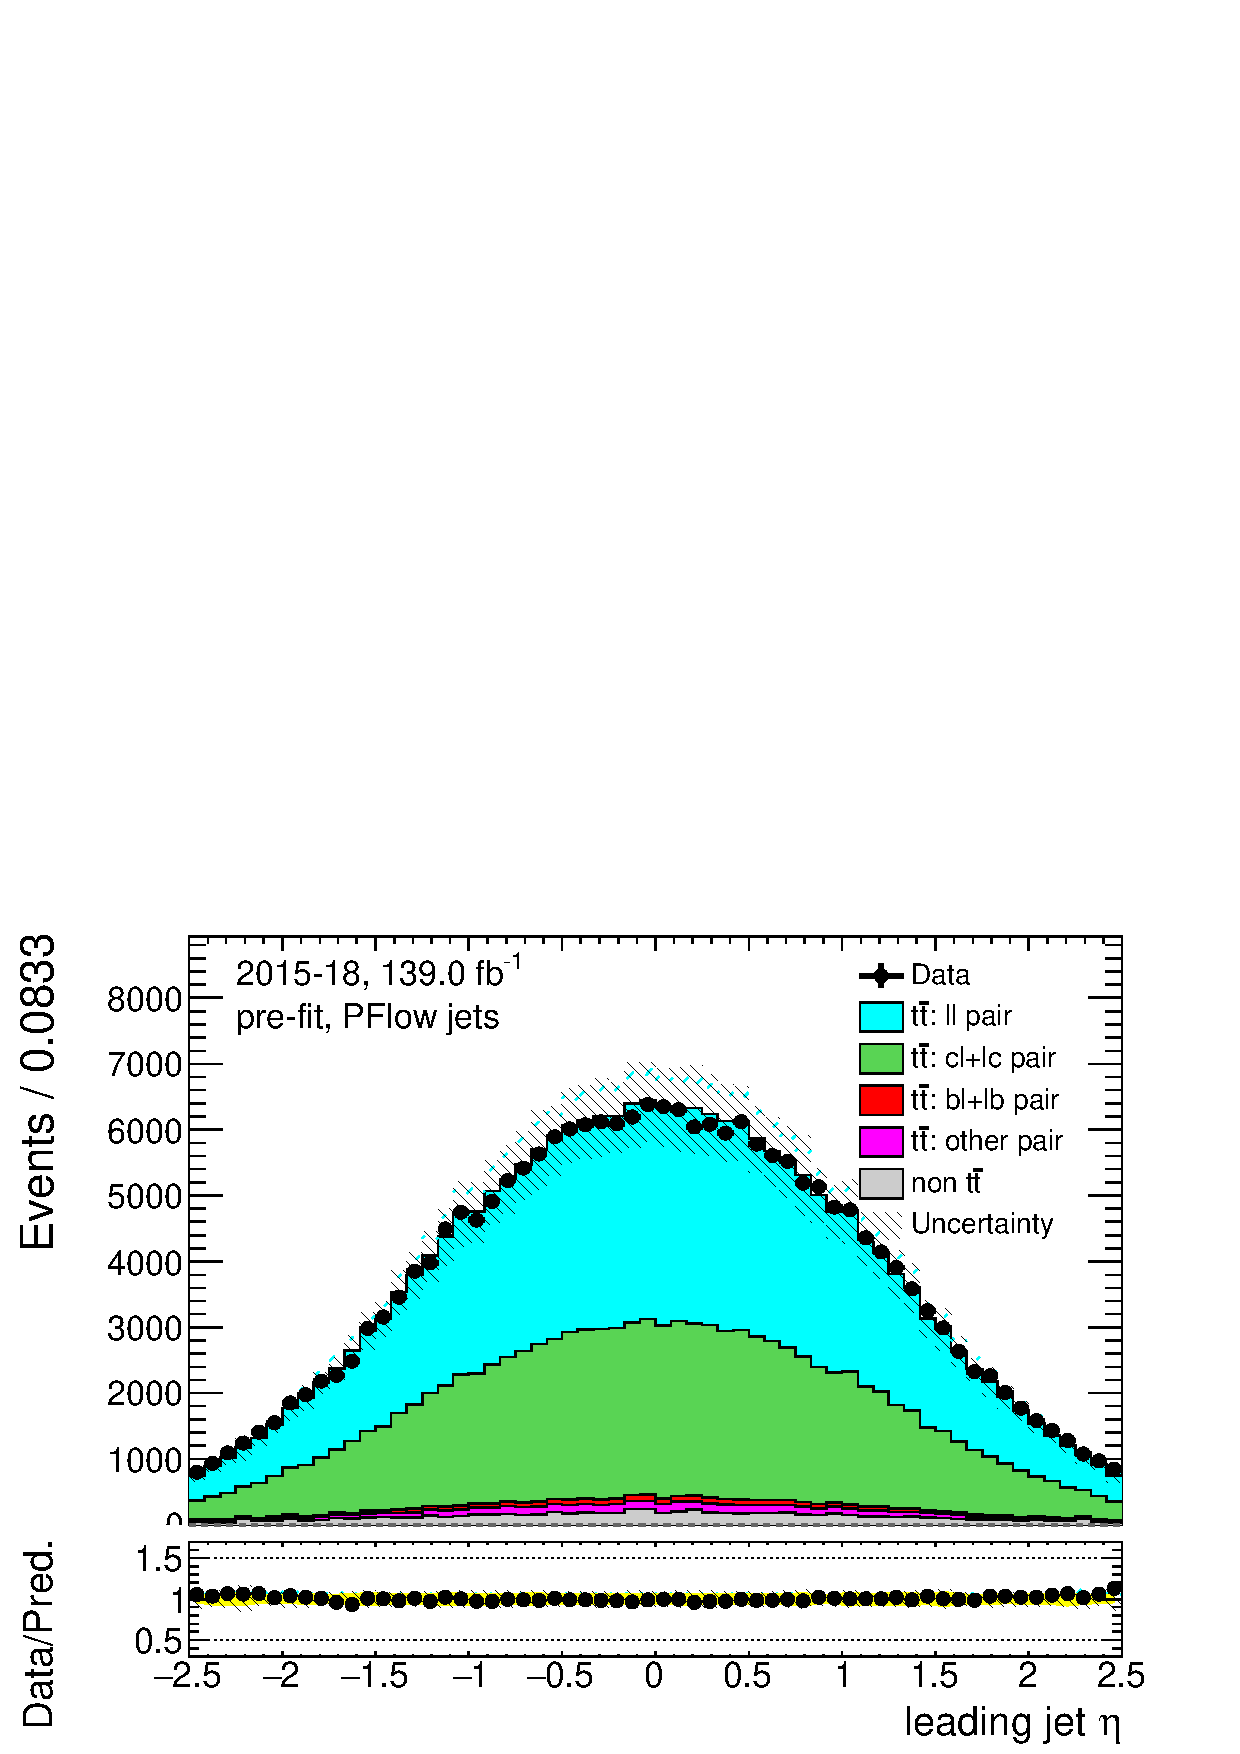
\includegraphics[width=.45\textwidth]{FTAG_plots/pretagNoRwwithouthighpTPFlowall/DataMC_h_J0_eta.png}
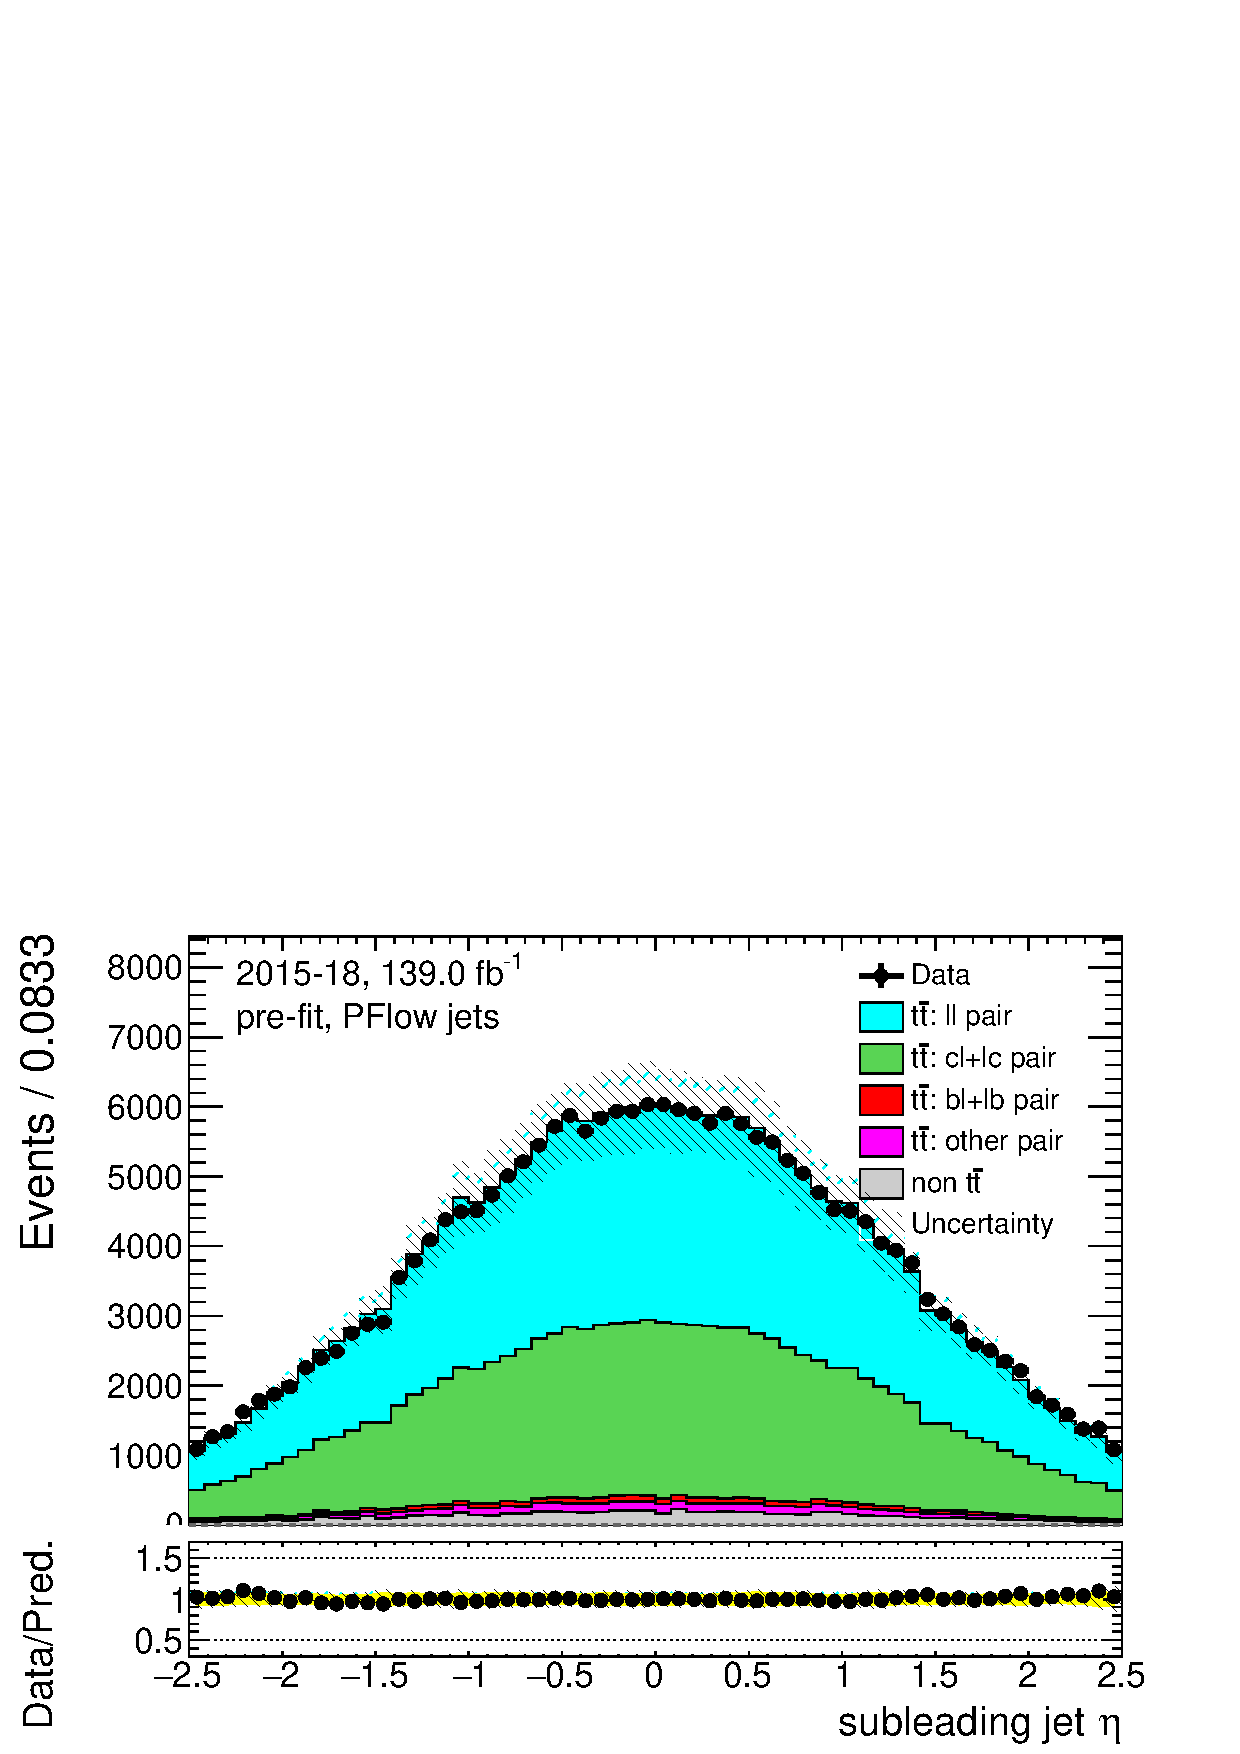
\includegraphics[width=.45\textwidth]{FTAG_plots/pretagNoRwwithouthighpTPFlowall/DataMC_h_J1_eta.png}\\
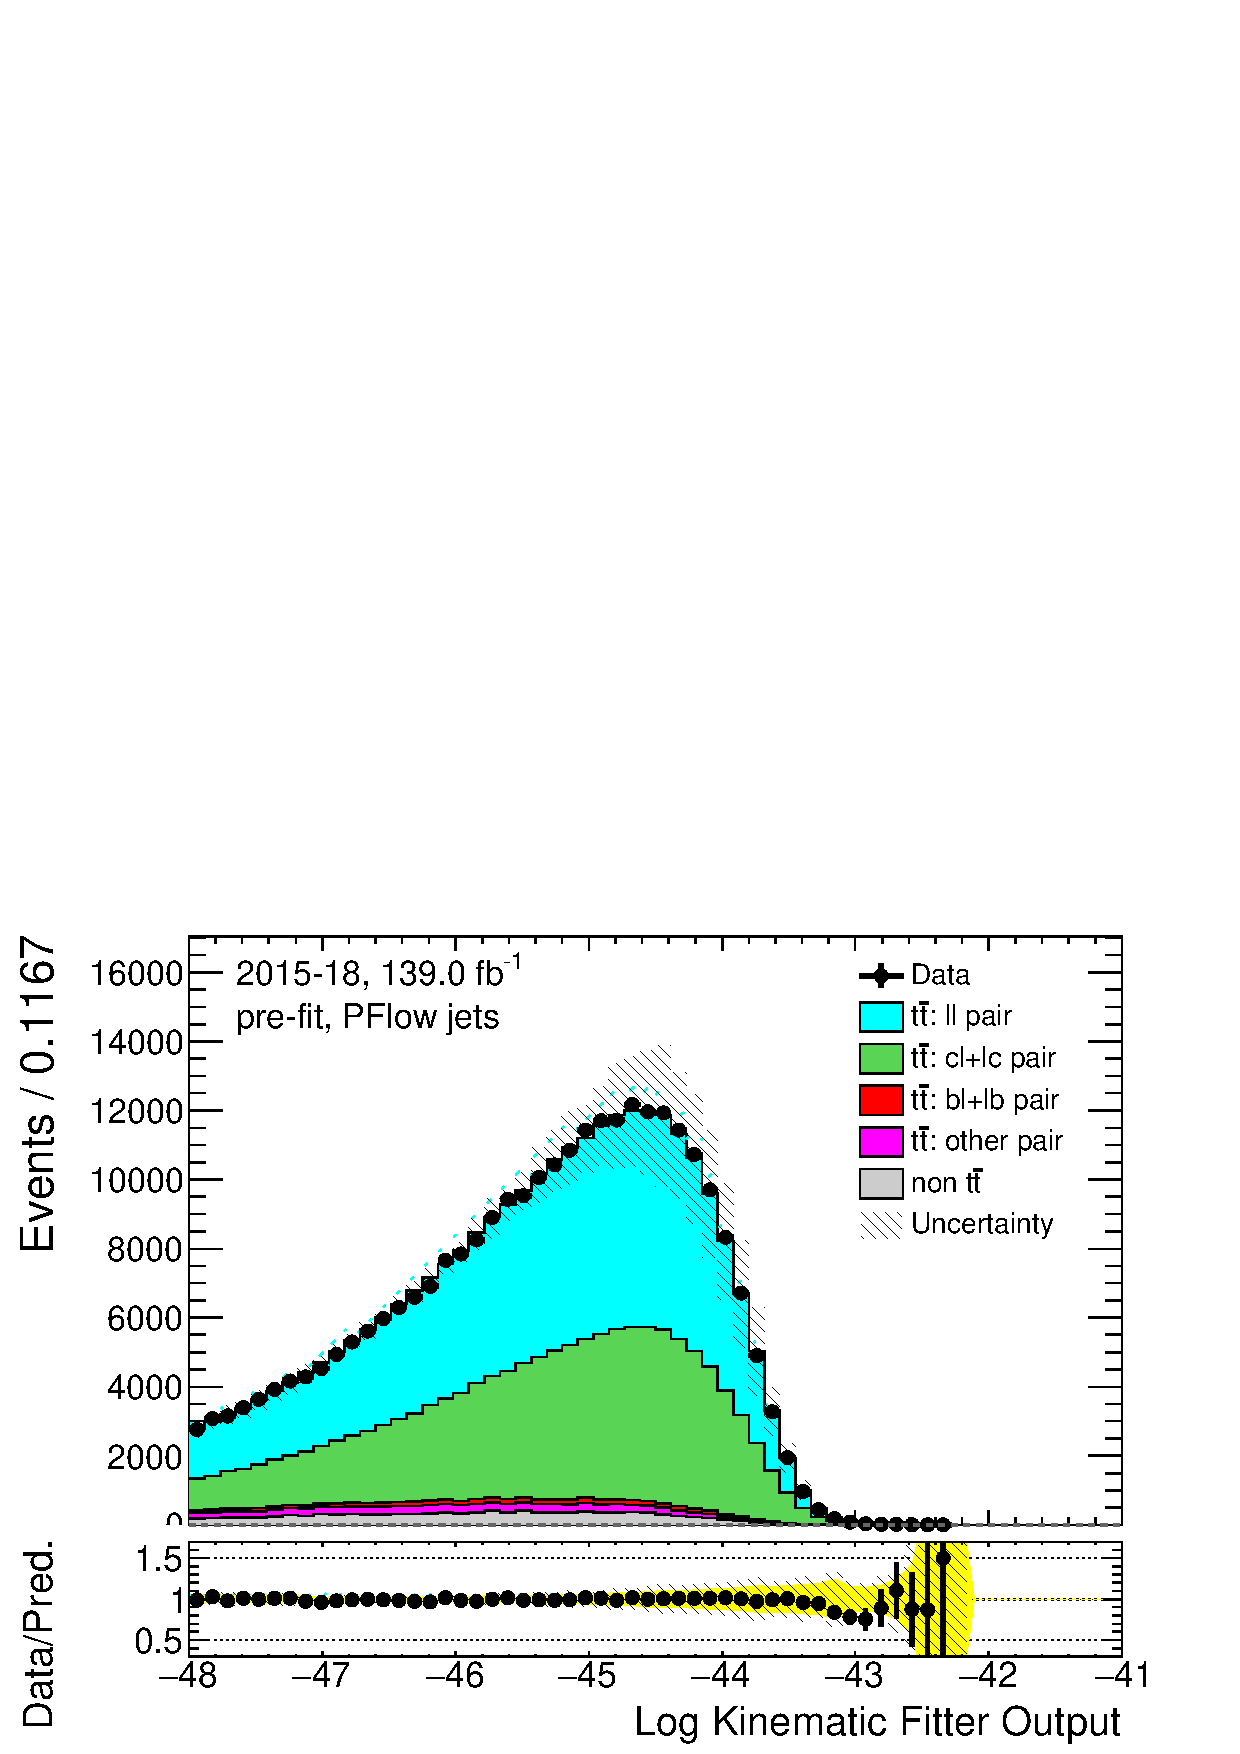
\includegraphics[width=.45\textwidth]{FTAG_plots/pretagNoRwwithouthighpTPFlowall/DataMC_h_LLR.png}
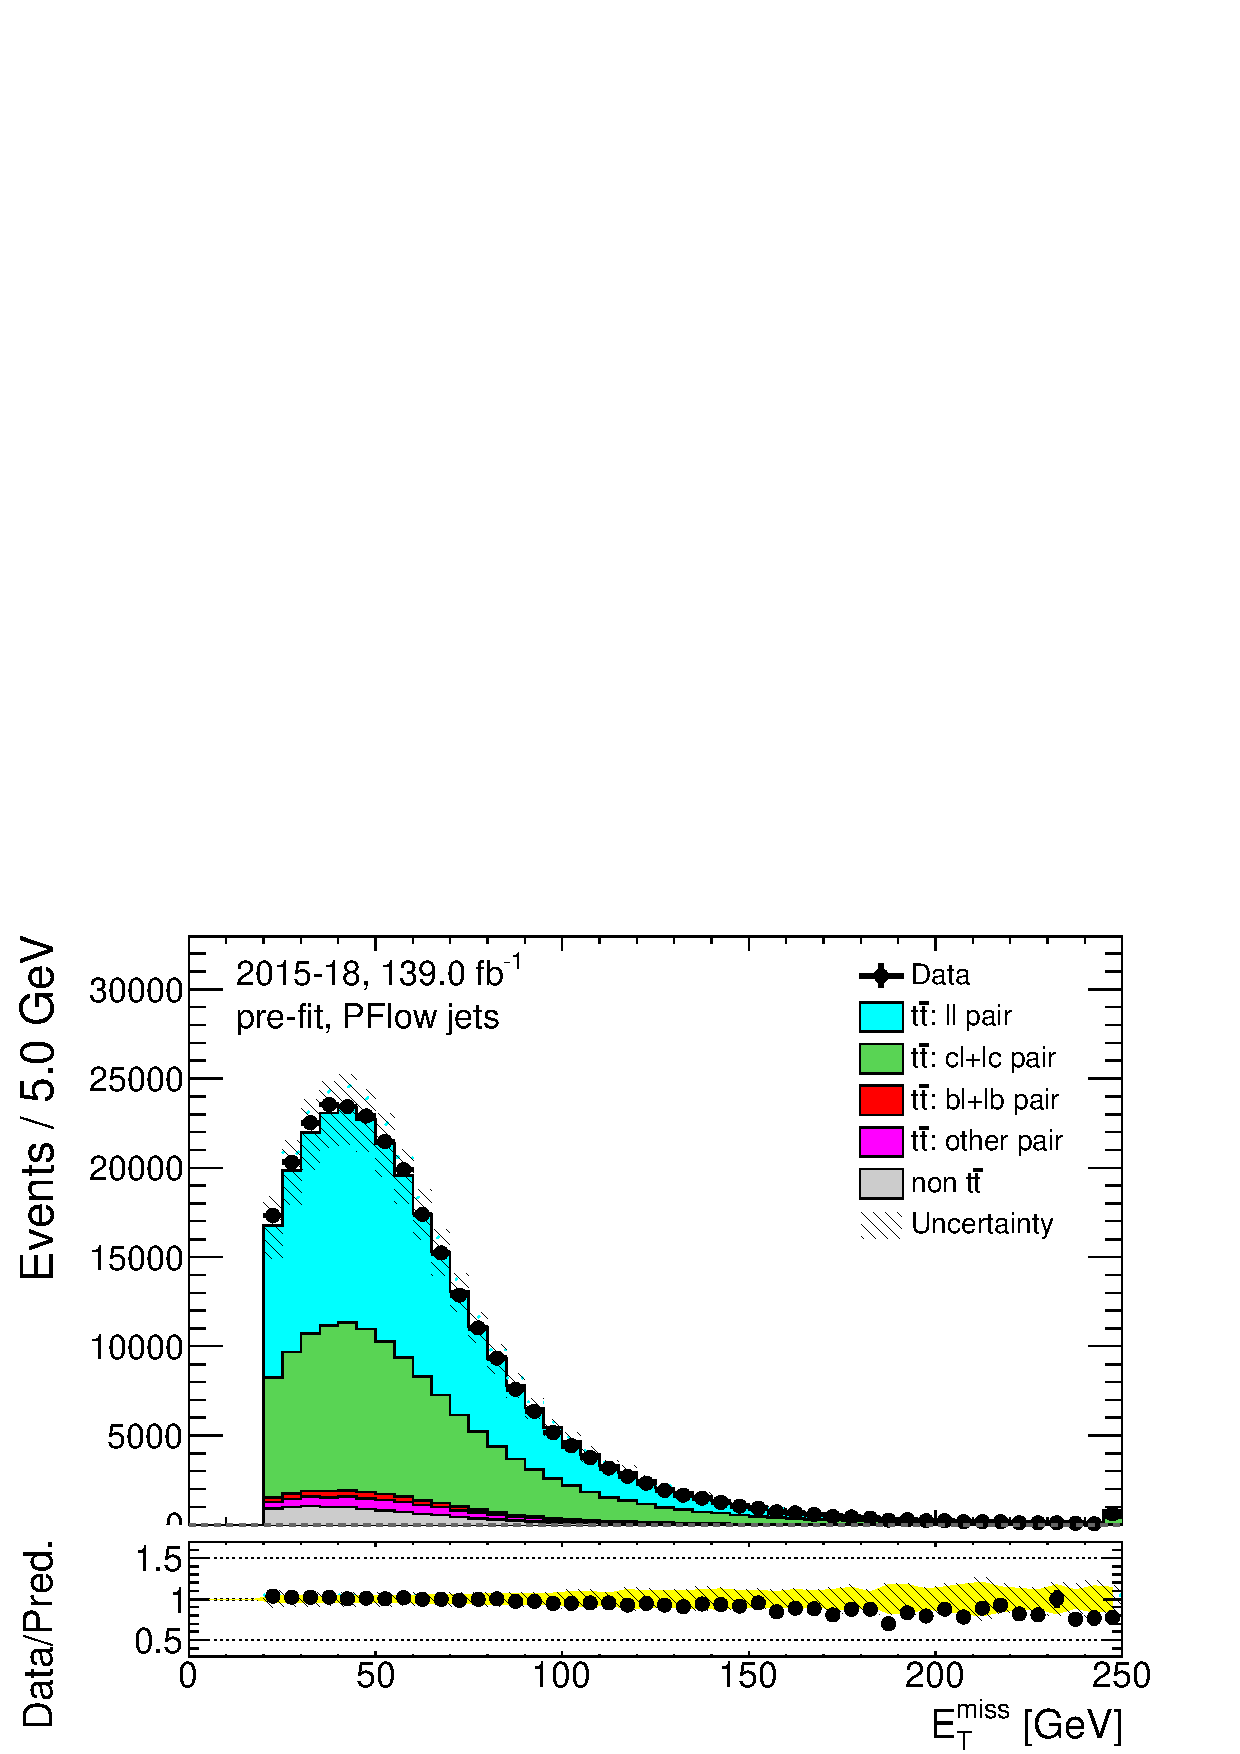
\includegraphics[width=.45\textwidth]{FTAG_plots/pretagNoRwwithouthighpTPFlowall/DataMC_h_MET.png}\\

\caption{PFlow jets: distributions of the leading and sub-leading jets 
from W decay, KLFitter output and the transverse missing transverse 
energy of the standard selection, before fitting or tagging with 
full uncertainties.} \label{fig:standard_jets_PFlow}
\end{figure}

\newpage
\begin{figure}[H]
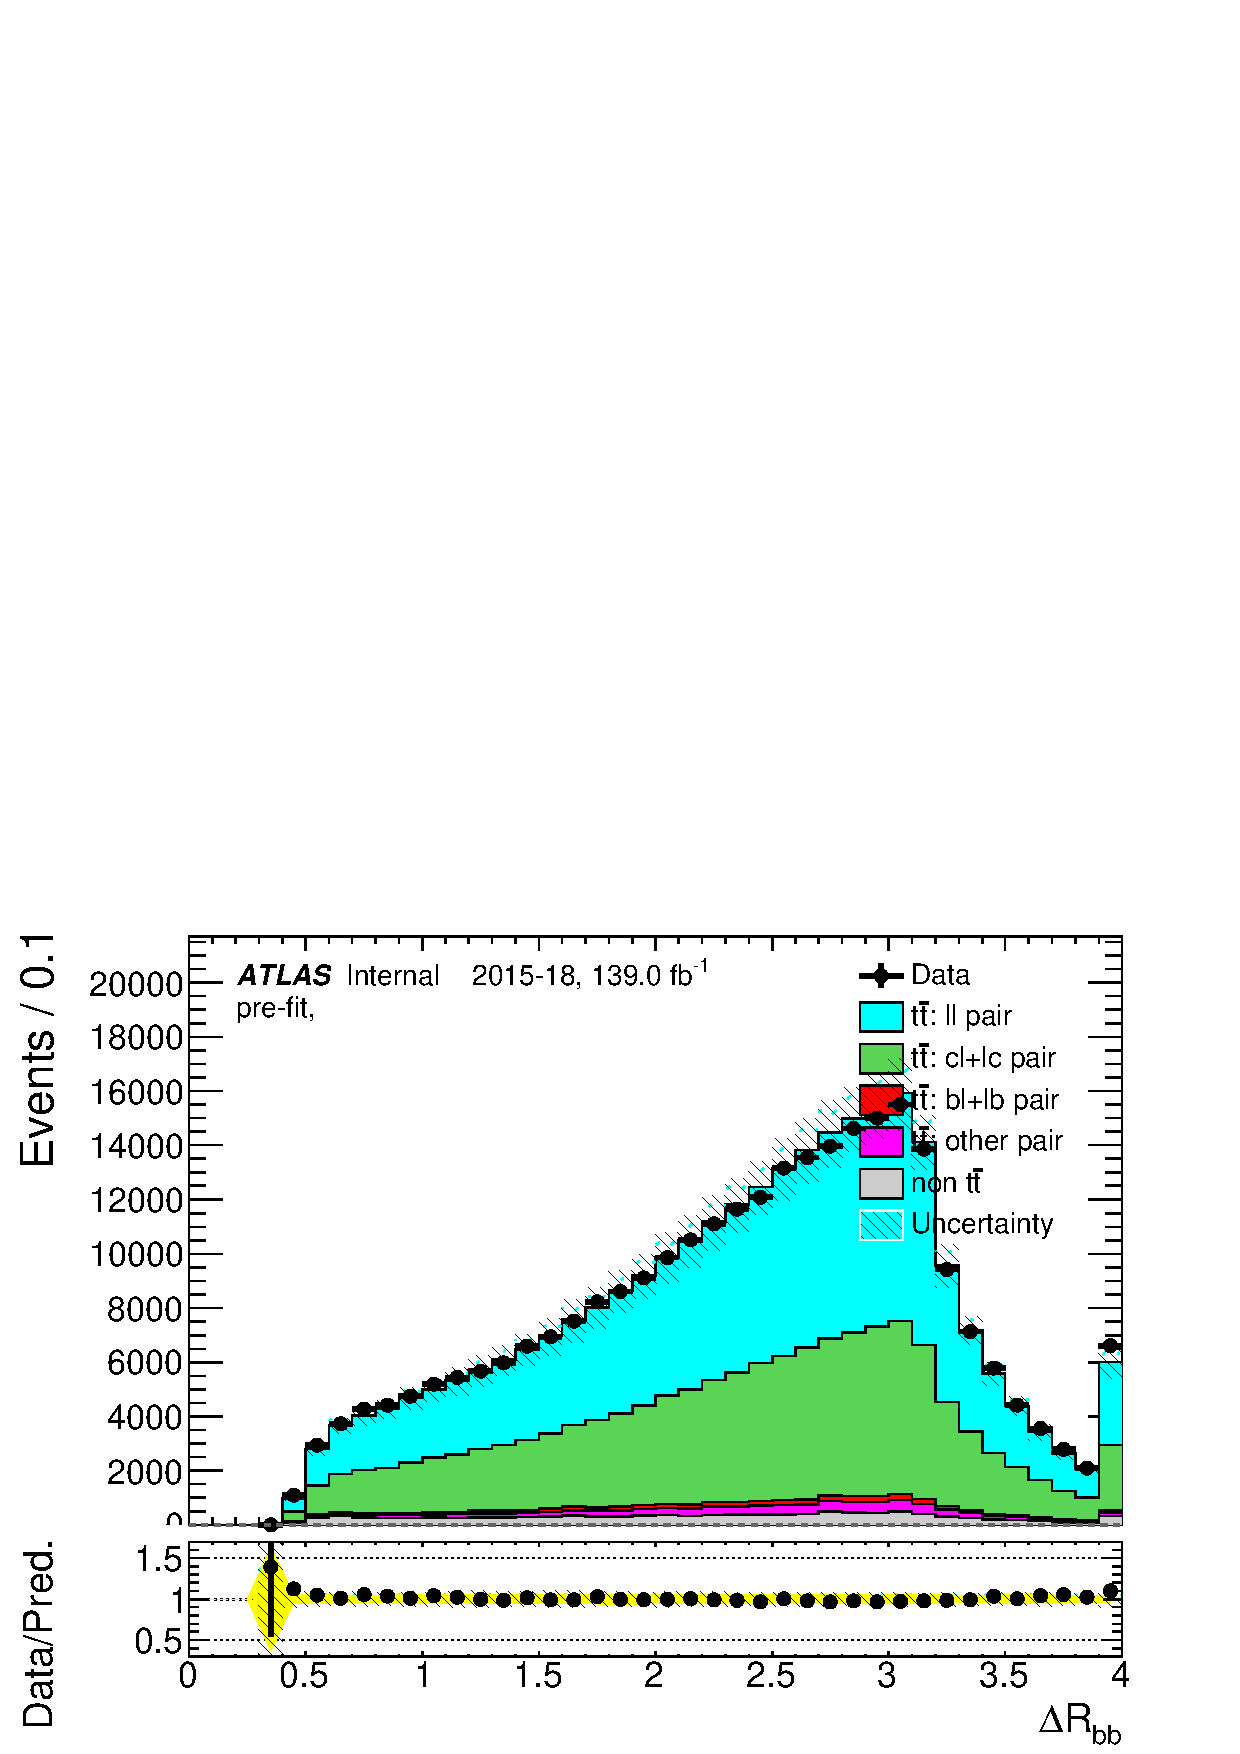
\includegraphics[width=.45\textwidth]{FTAG_plots/pretagNoRwwithouthighpTPFlowall/DataMC_h_dRbb.png}
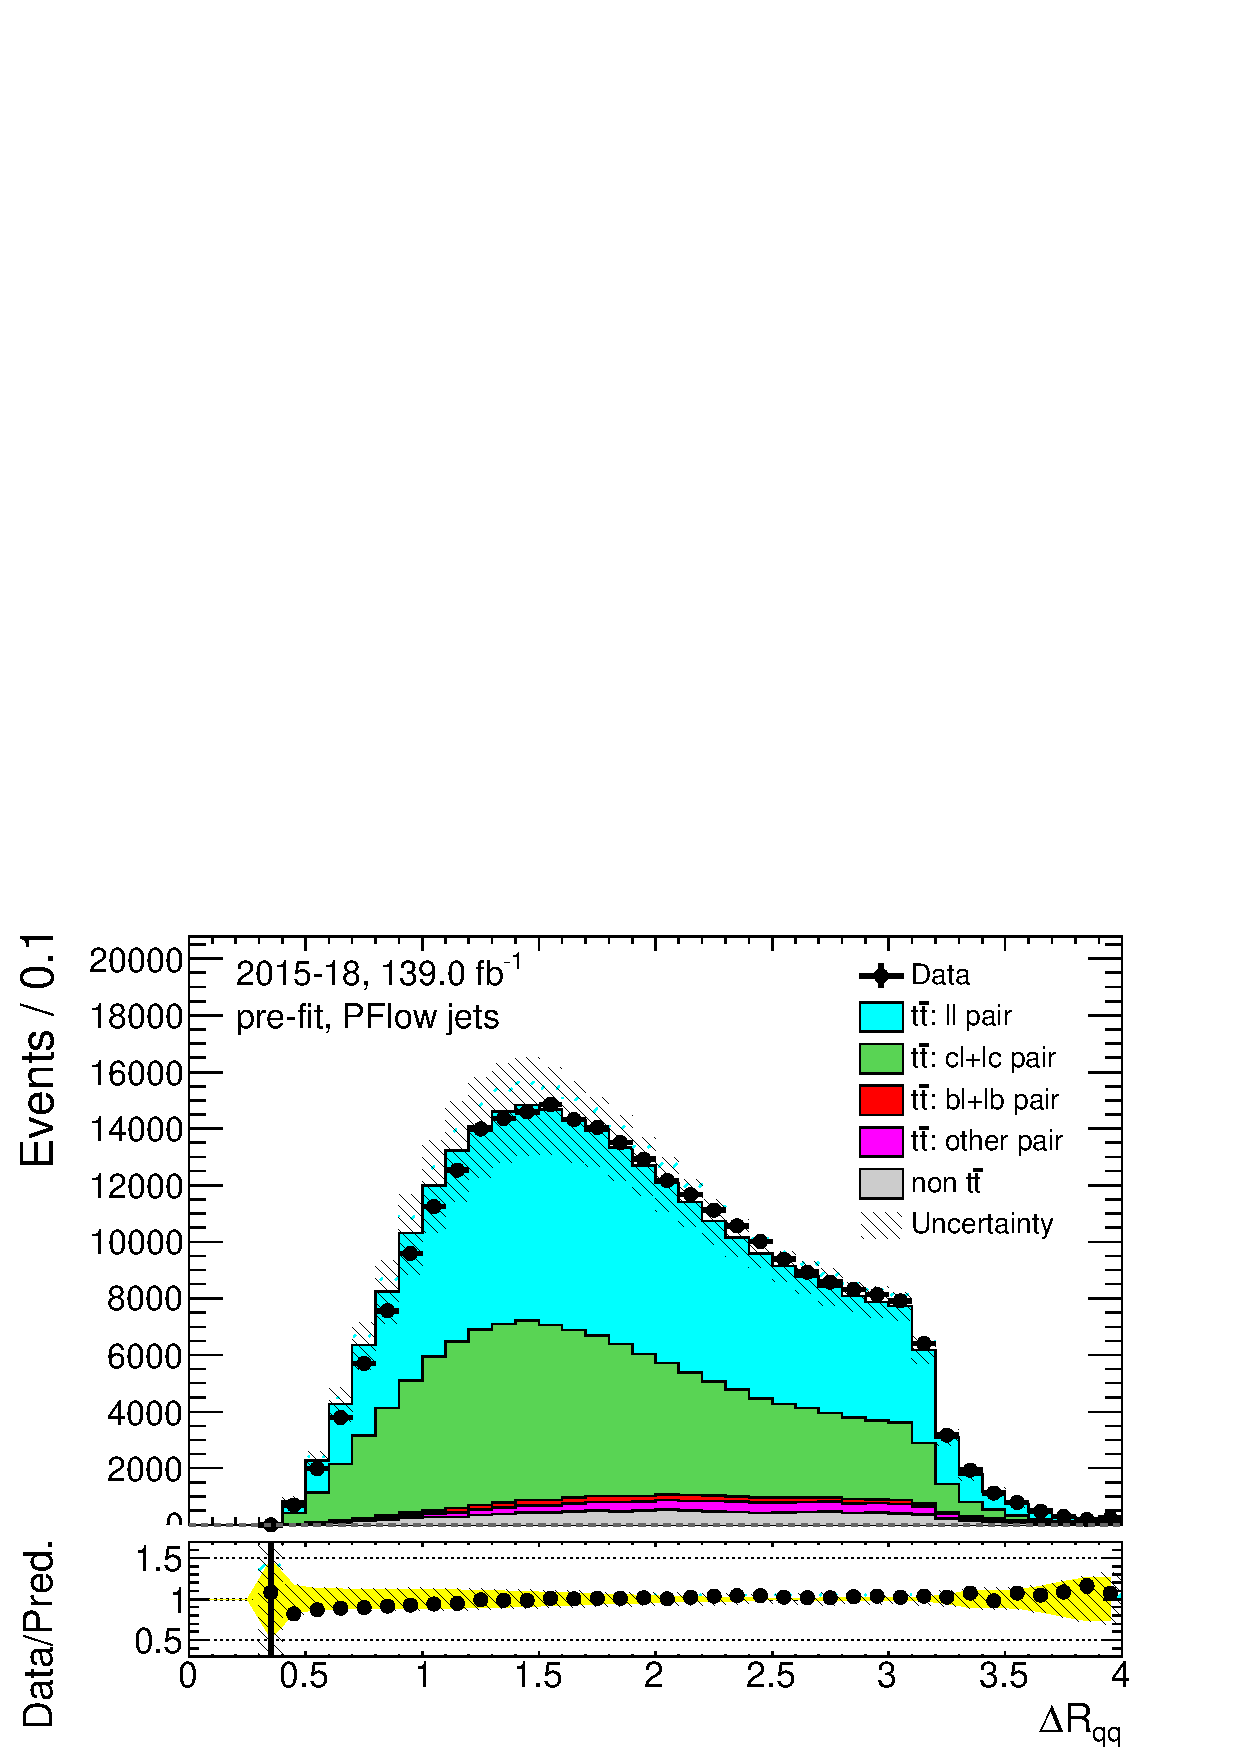
\includegraphics[width=.45\textwidth]{FTAG_plots/pretagNoRwwithouthighpTPFlowall/DataMC_h_dRqq.png}\\
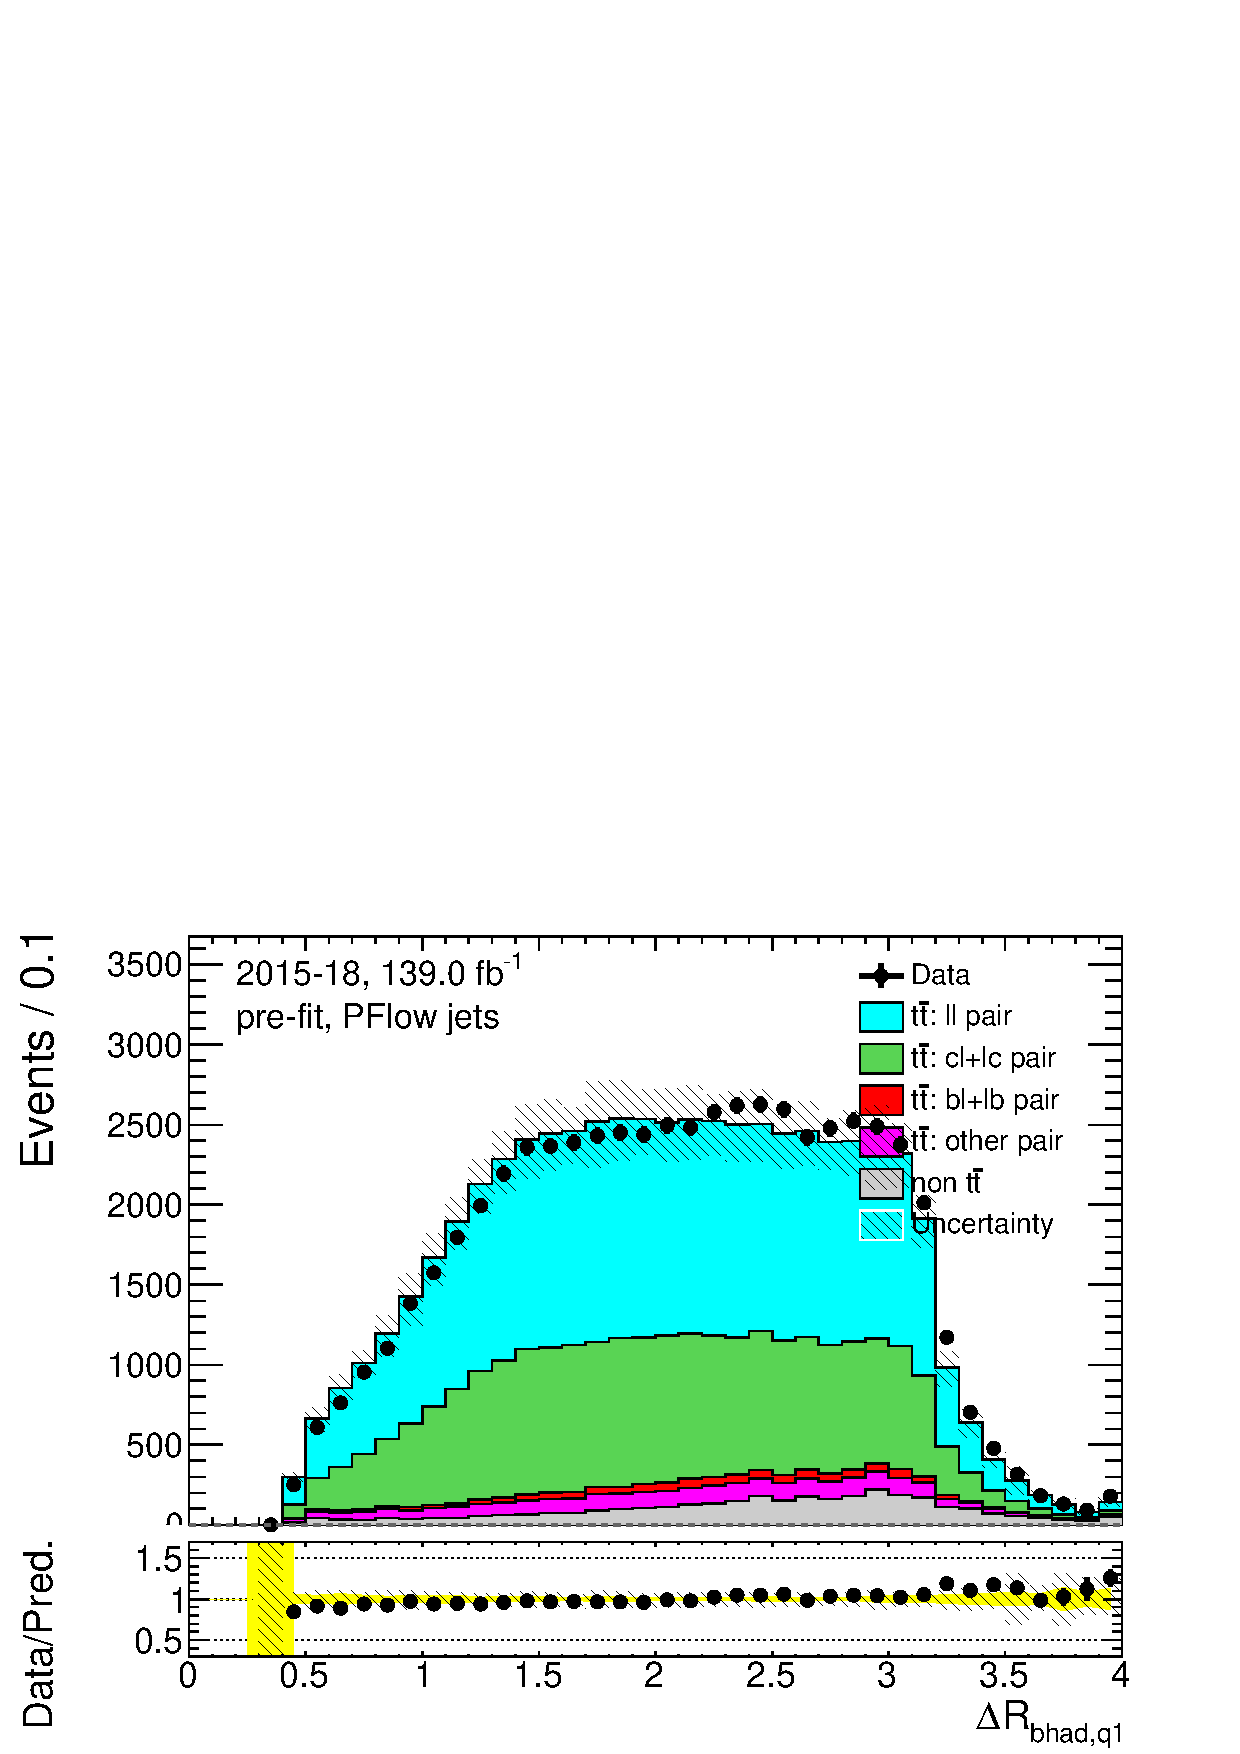
\includegraphics[width=.45\textwidth]{FTAG_plots/pretagNoRwwithouthighpTPFlowall/DataMC_h_dRbhadq1.png}
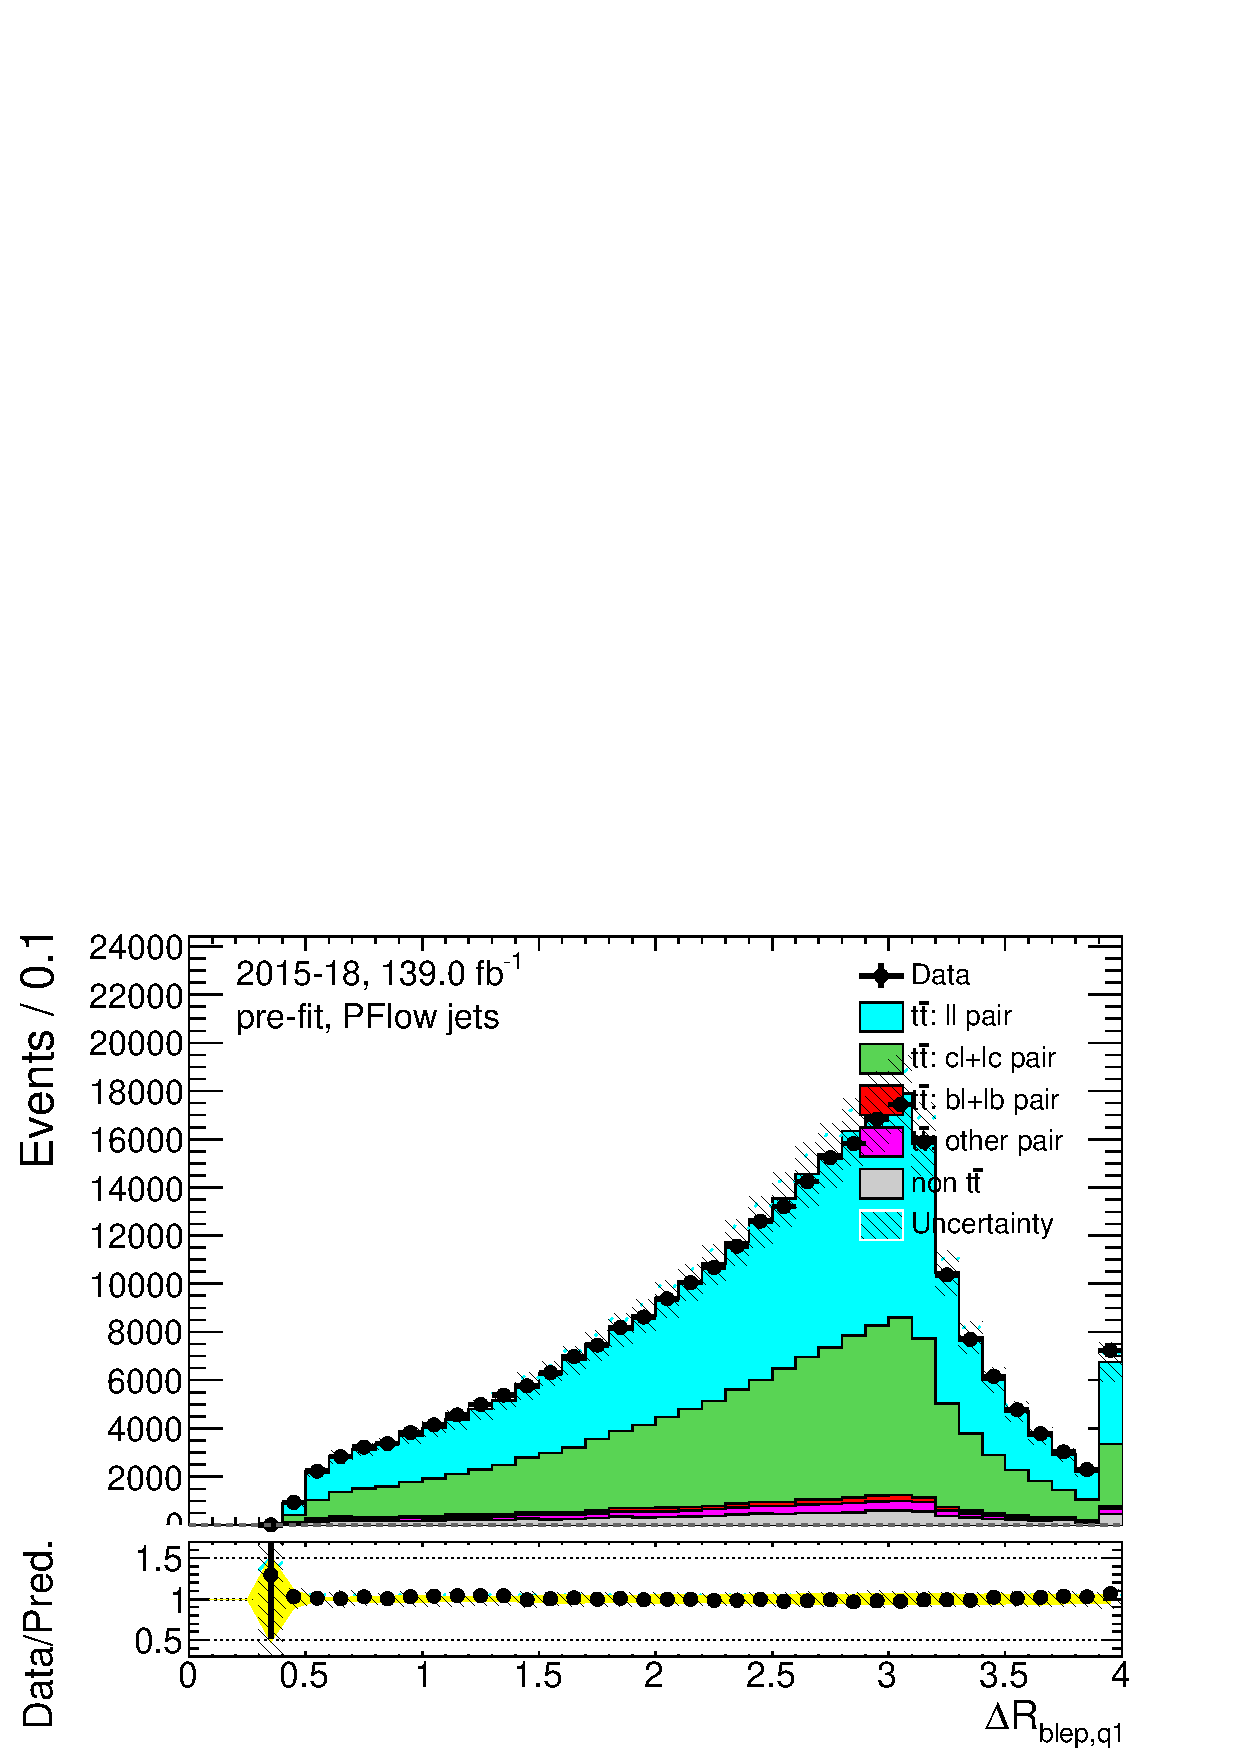
\includegraphics[width=.45\textwidth]{FTAG_plots/pretagNoRwwithouthighpTPFlowall/DataMC_h_dRblepq1.png} \\
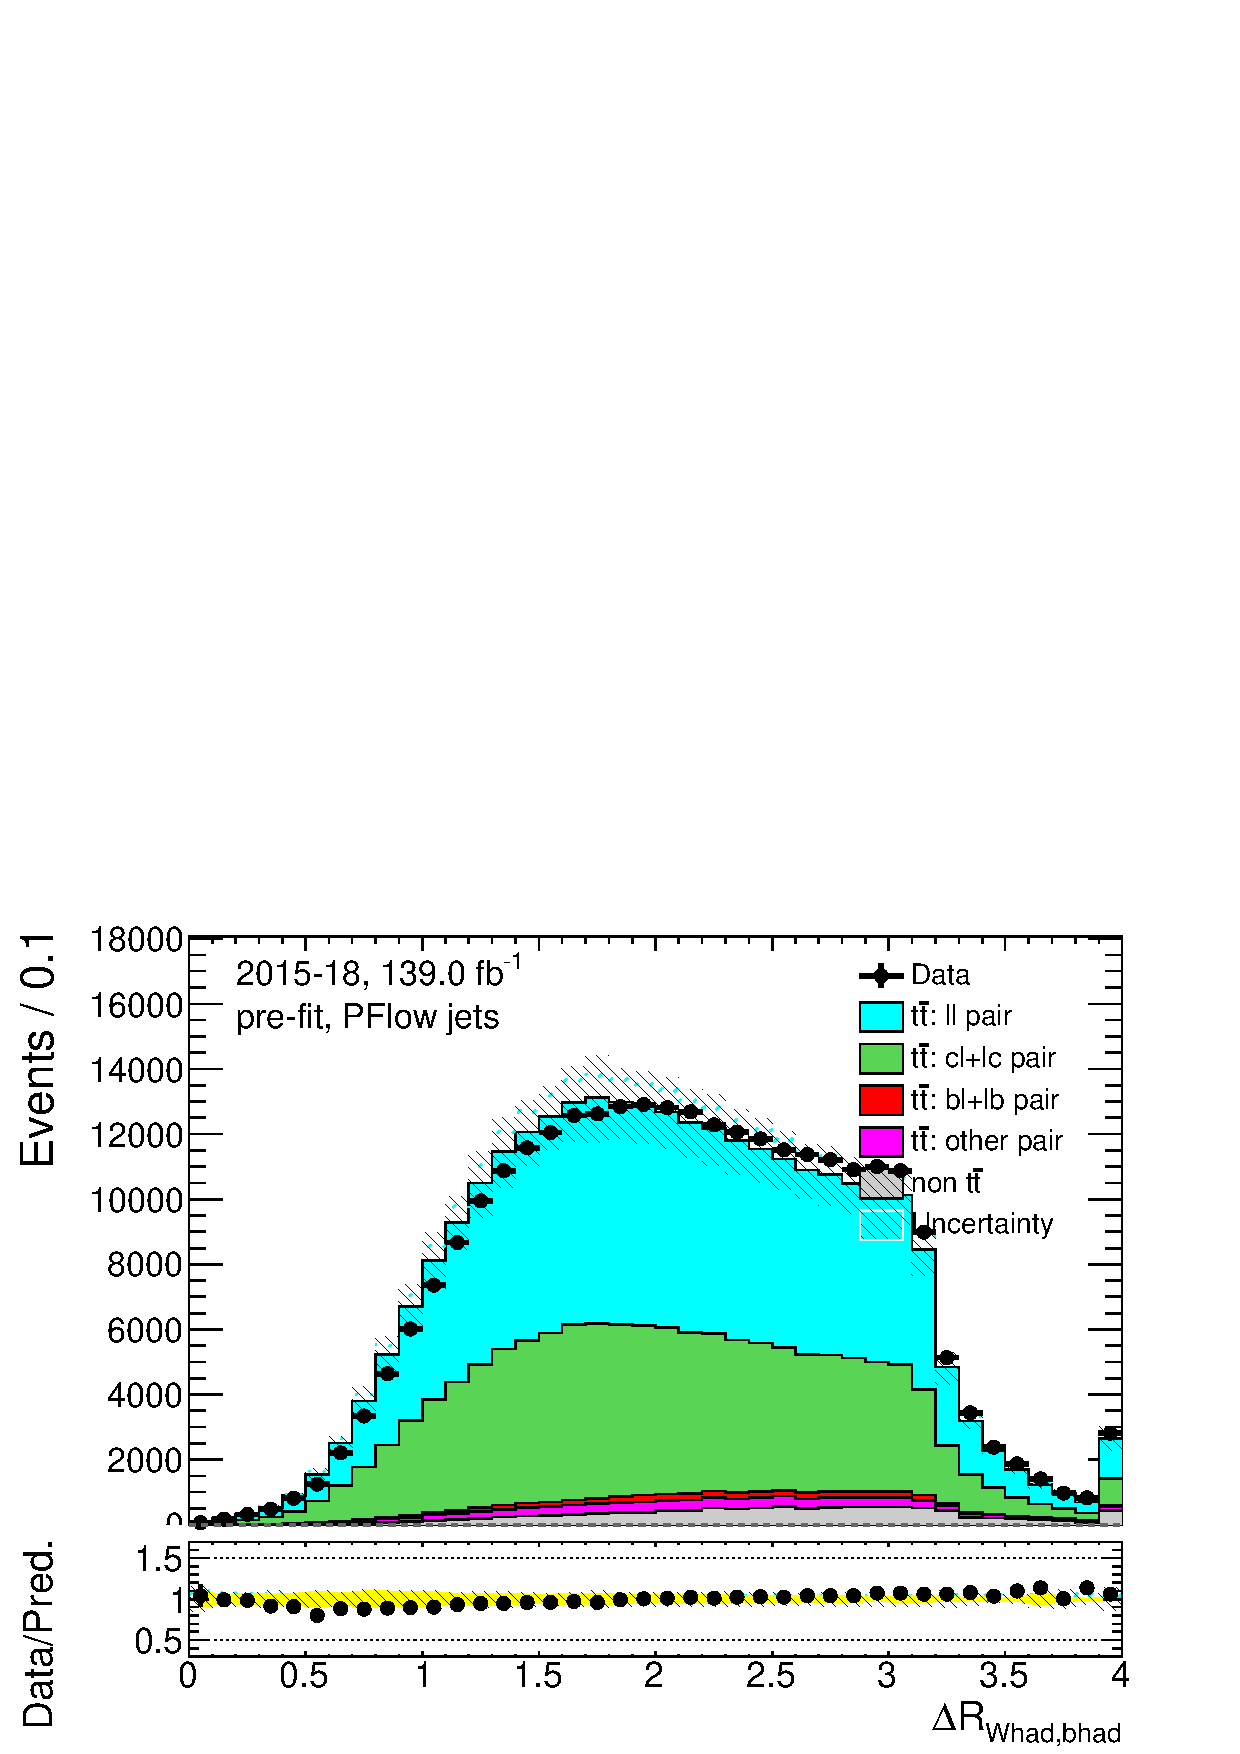
\includegraphics[width=.45\textwidth]{FTAG_plots/pretagNoRwwithouthighpTPFlowall/DataMC_h_dRWhadbhad.png} 
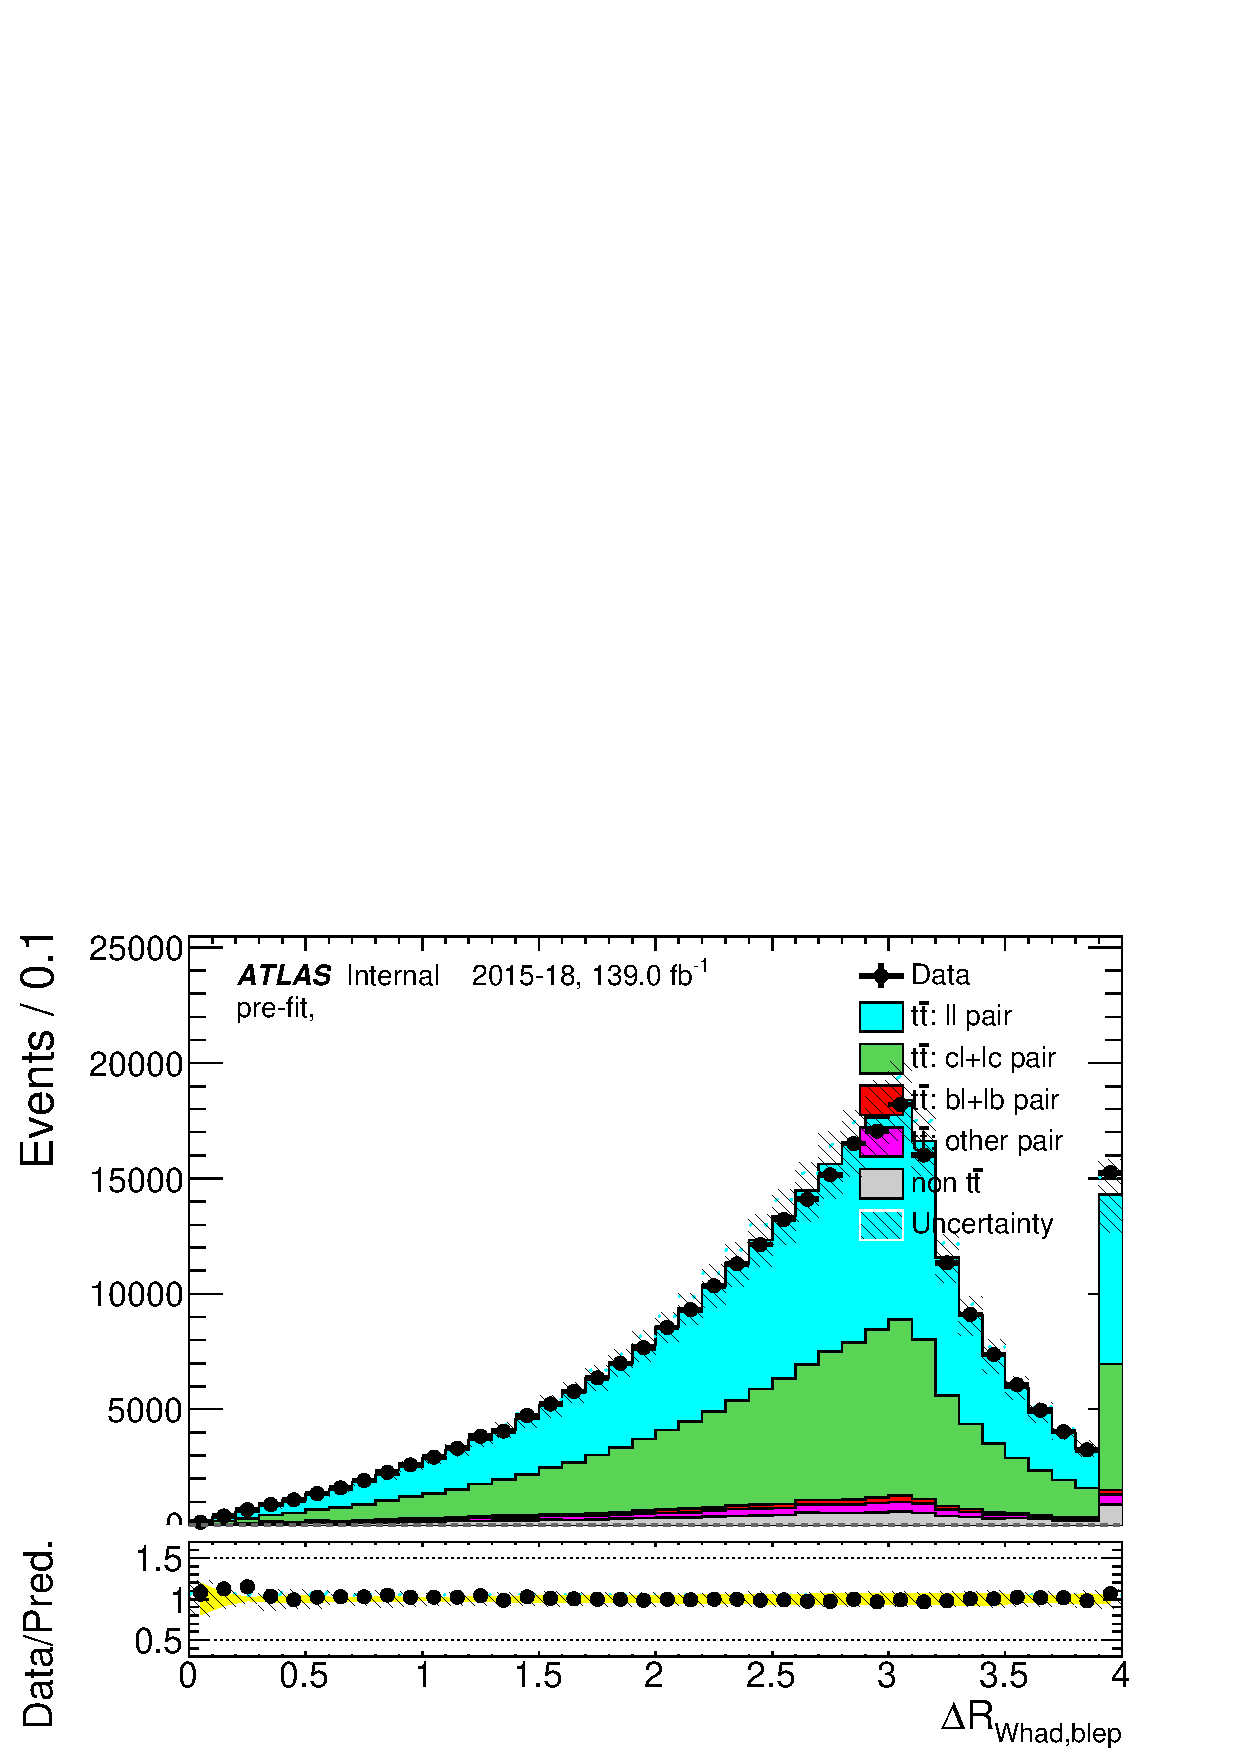
\includegraphics[width=.45\textwidth]{FTAG_plots/pretagNoRwwithouthighpTPFlowall/DataMC_h_dRWhadblep.png} \\
\caption{PFlow jets: distributions of angle related variables of the combination of the standard selection,
 before fitting or 
tagging with full uncertainties.} \label{fig:standard_angles_PFlow}
\end{figure}

\newpage
\begin{figure}[H]
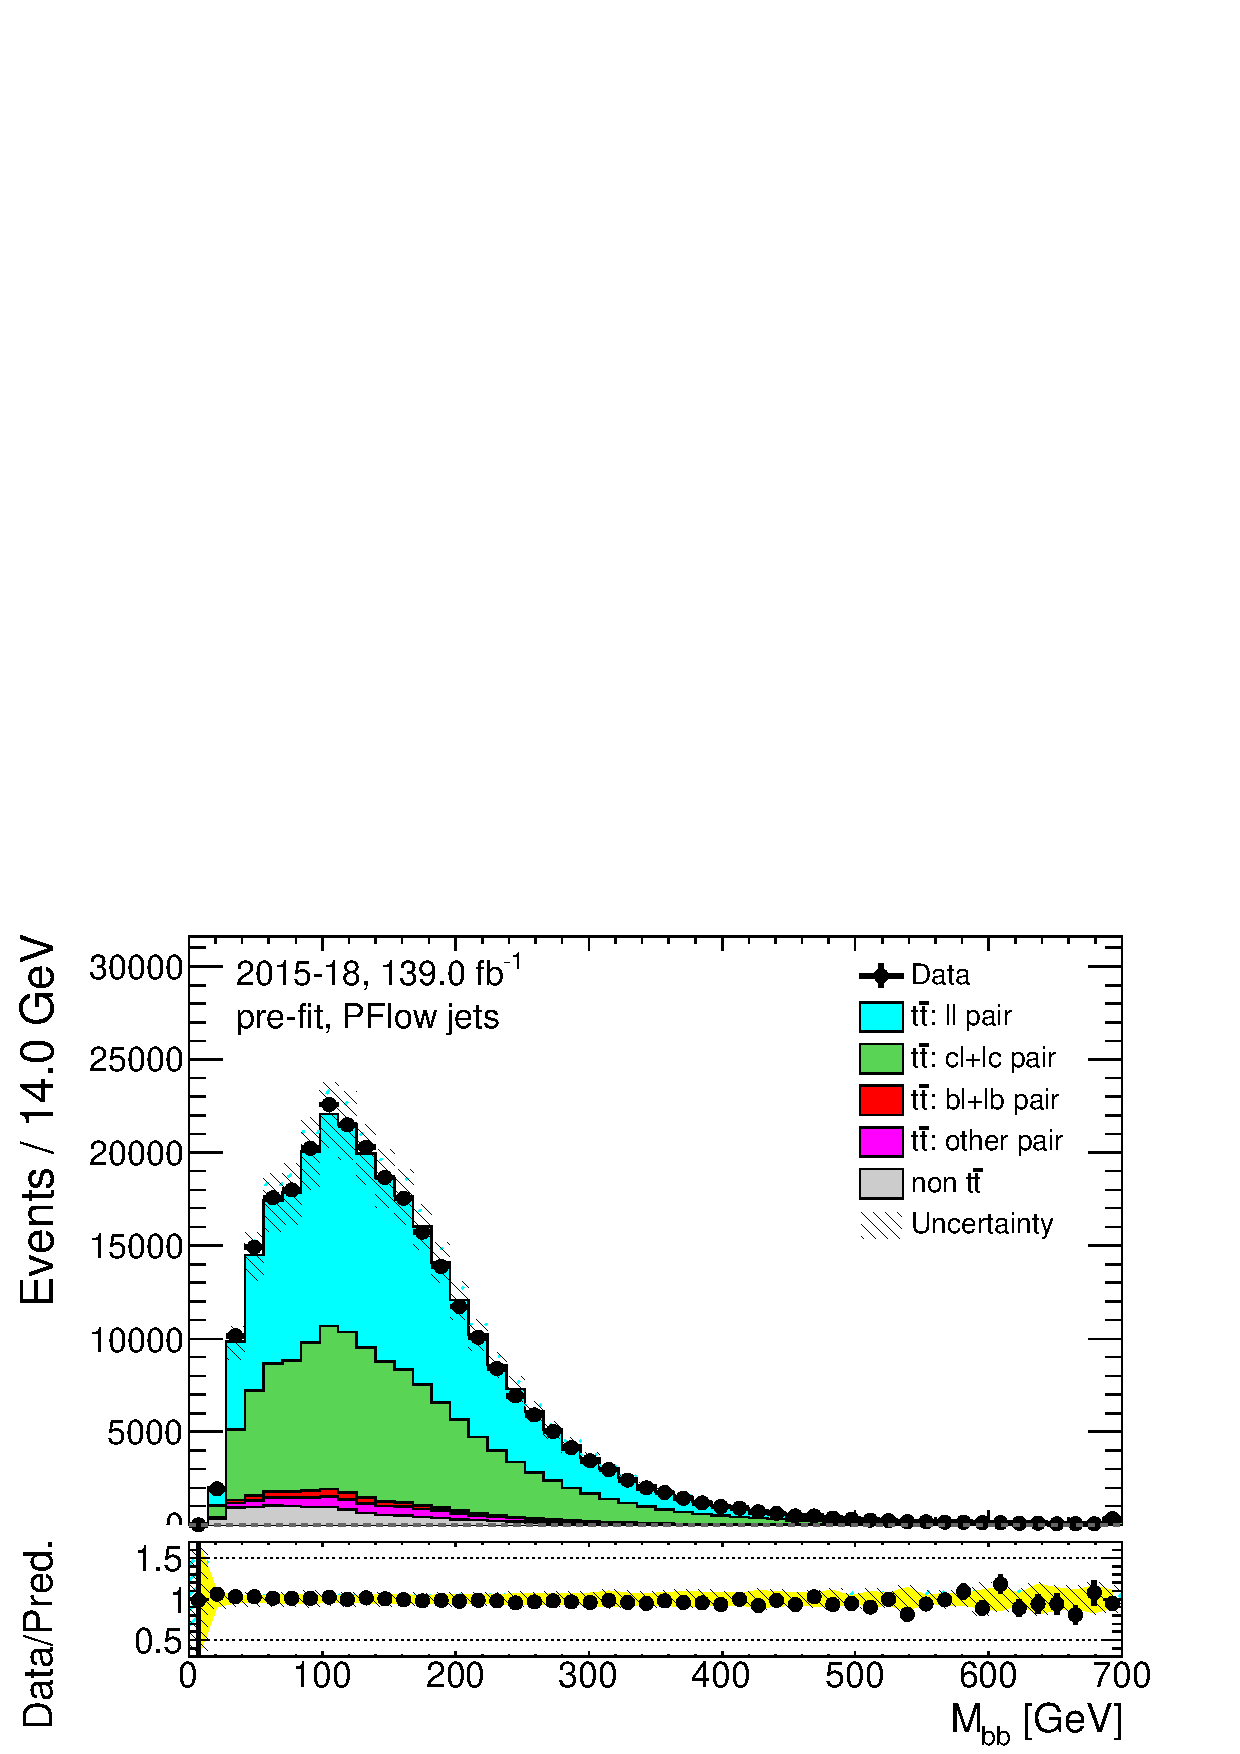
\includegraphics[width=.45\textwidth]{FTAG_plots/pretagNoRwwithouthighpTPFlowall/DataMC_h_Mbb.png}
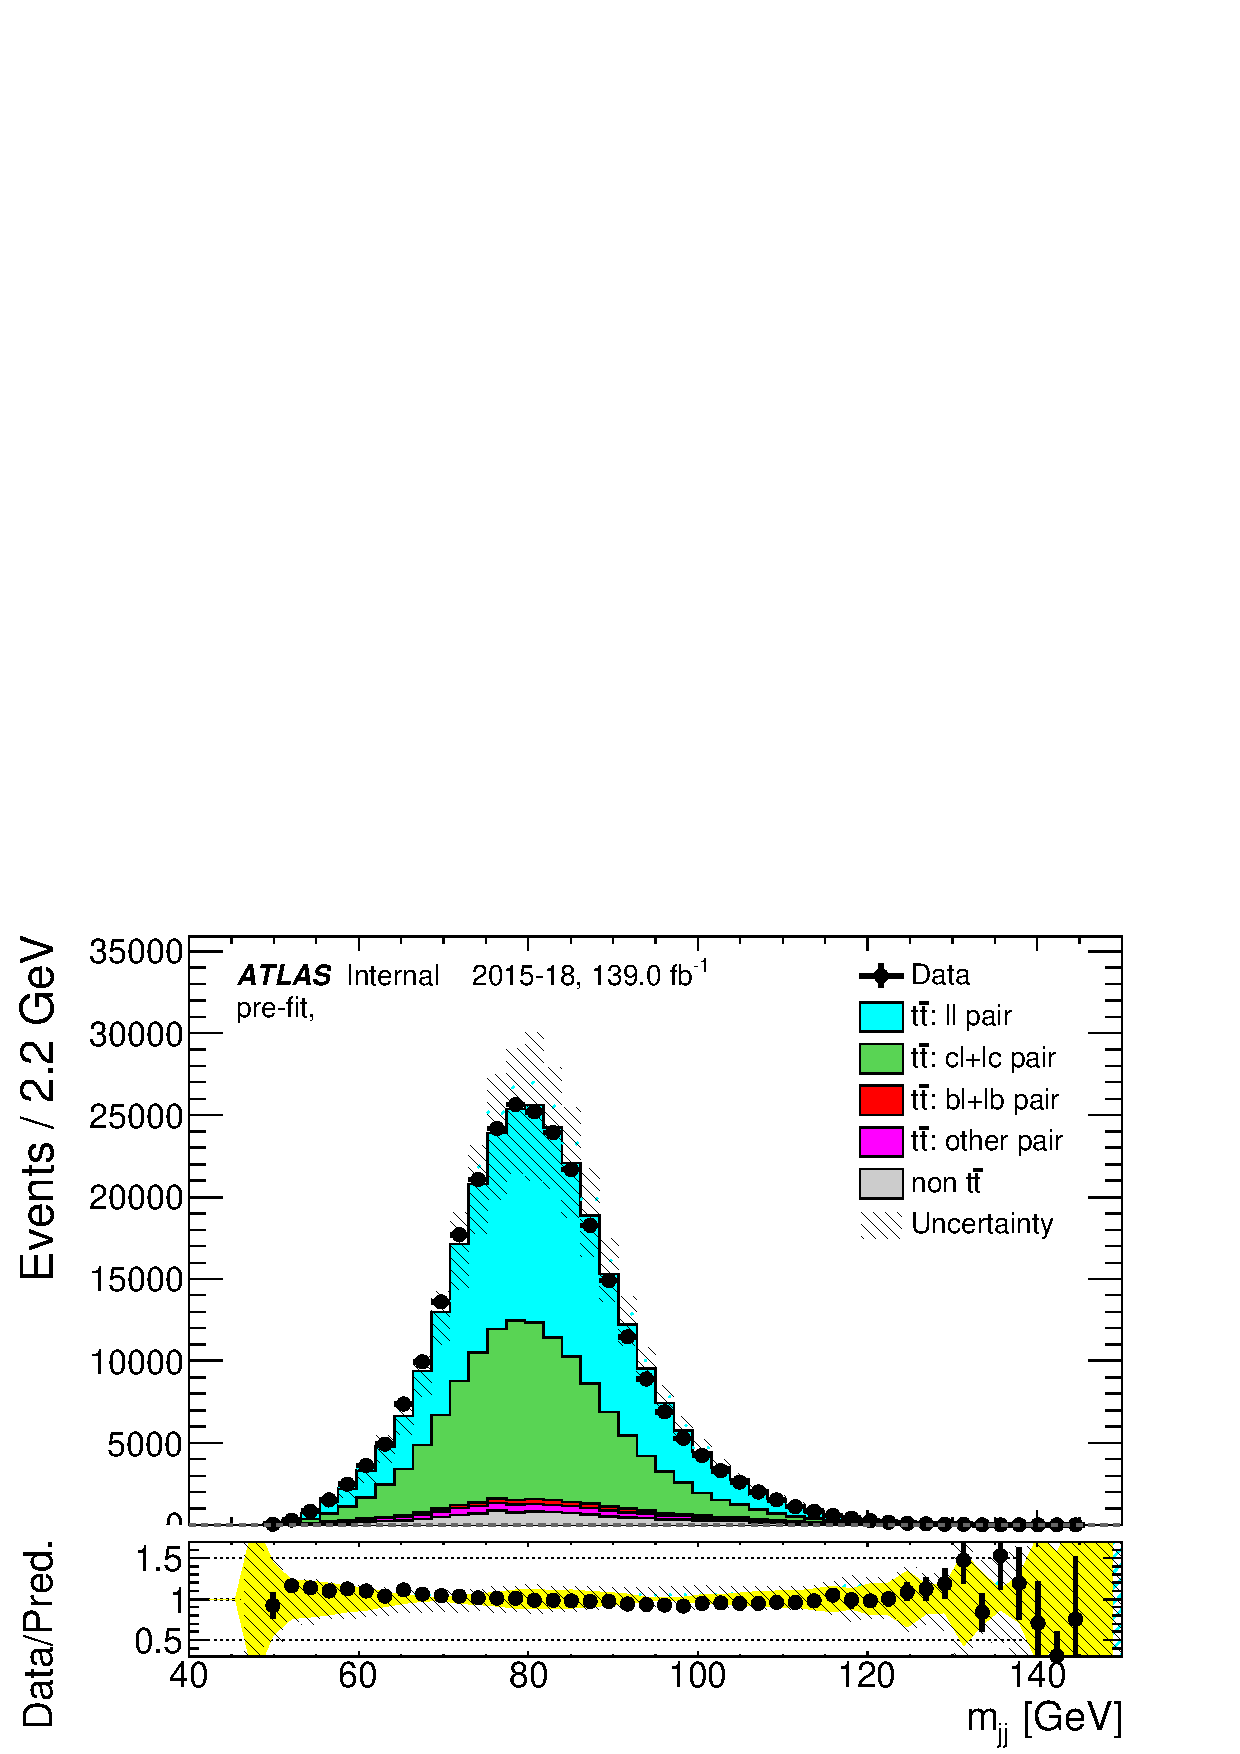
\includegraphics[width=.45\textwidth]{FTAG_plots/pretagNoRwwithouthighpTPFlowall/DataMC_h_mjj.png}\\
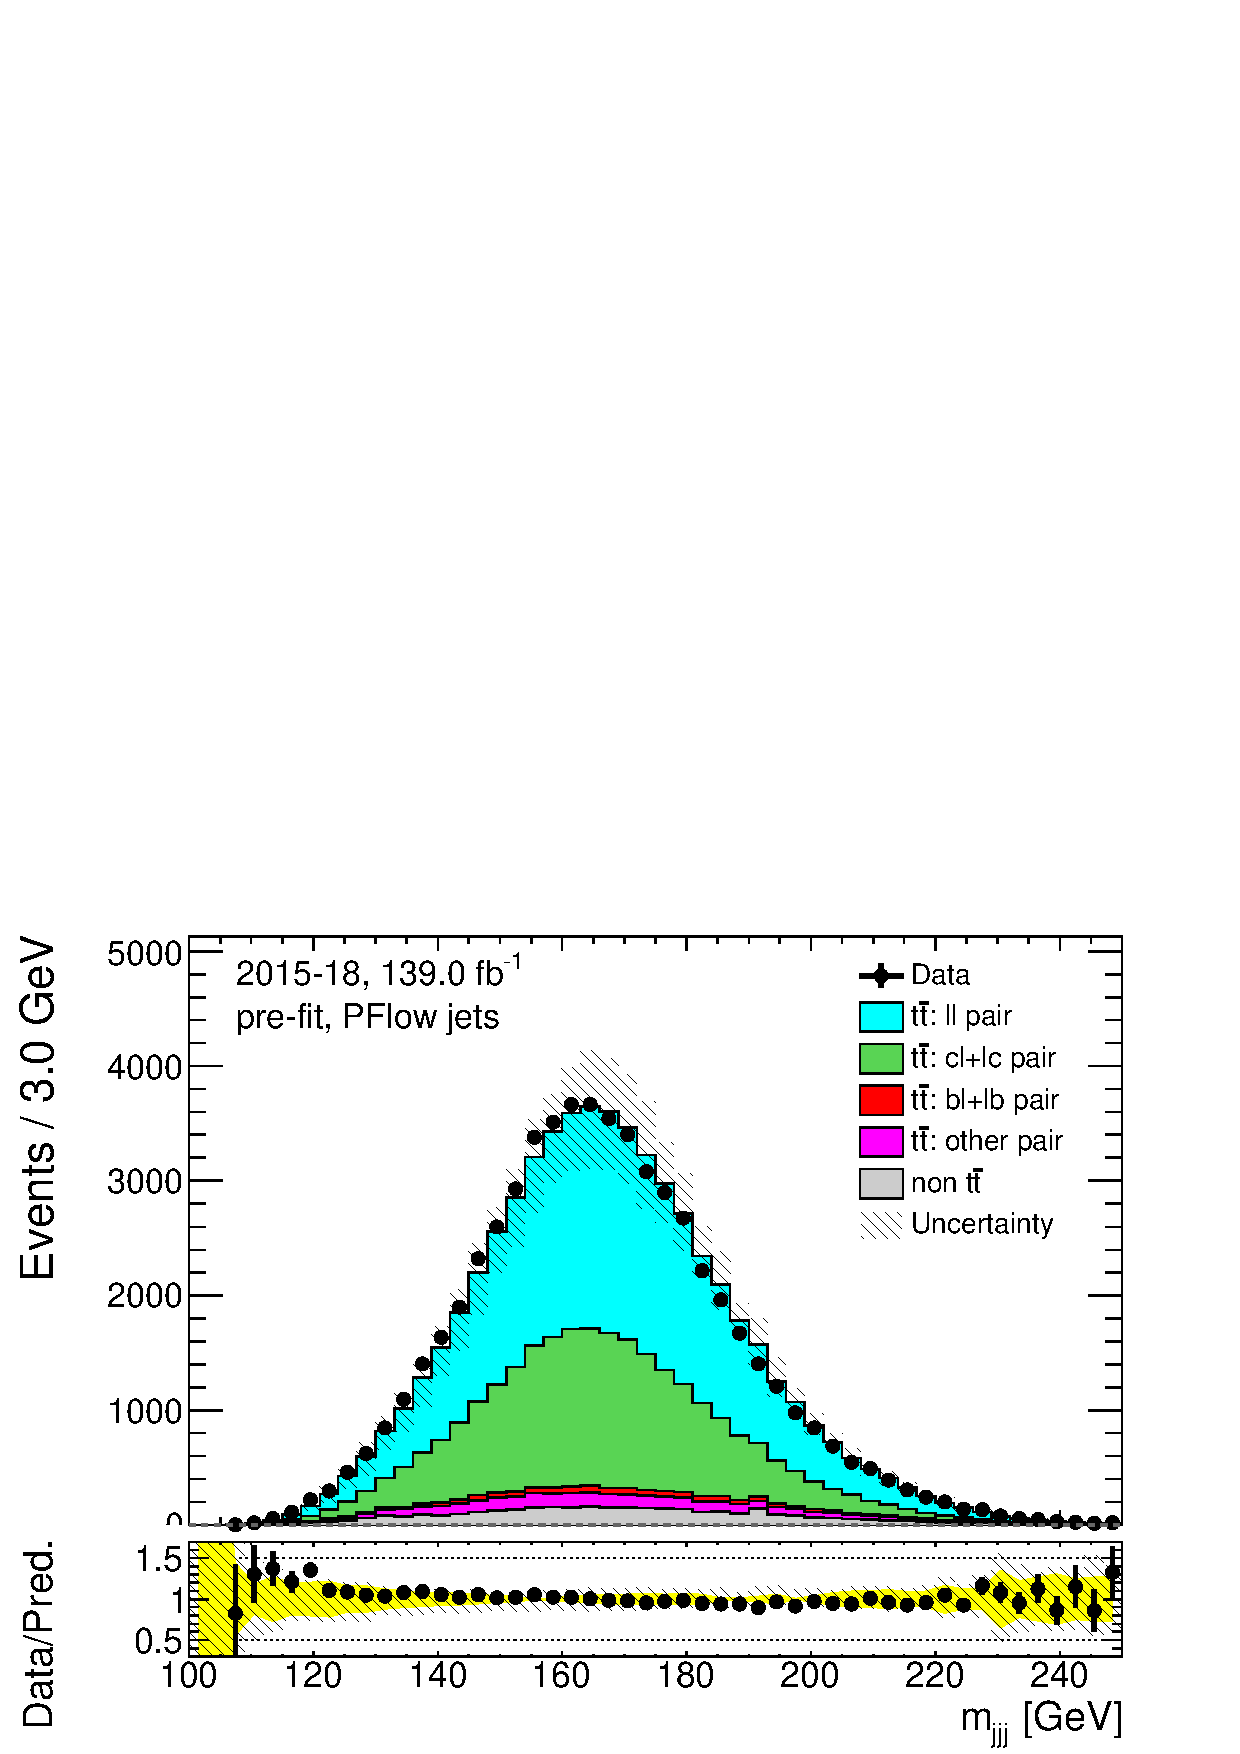
\includegraphics[width=.45\textwidth]{FTAG_plots/pretagNoRwwithouthighpTPFlowall/DataMC_h_mjjj.png}
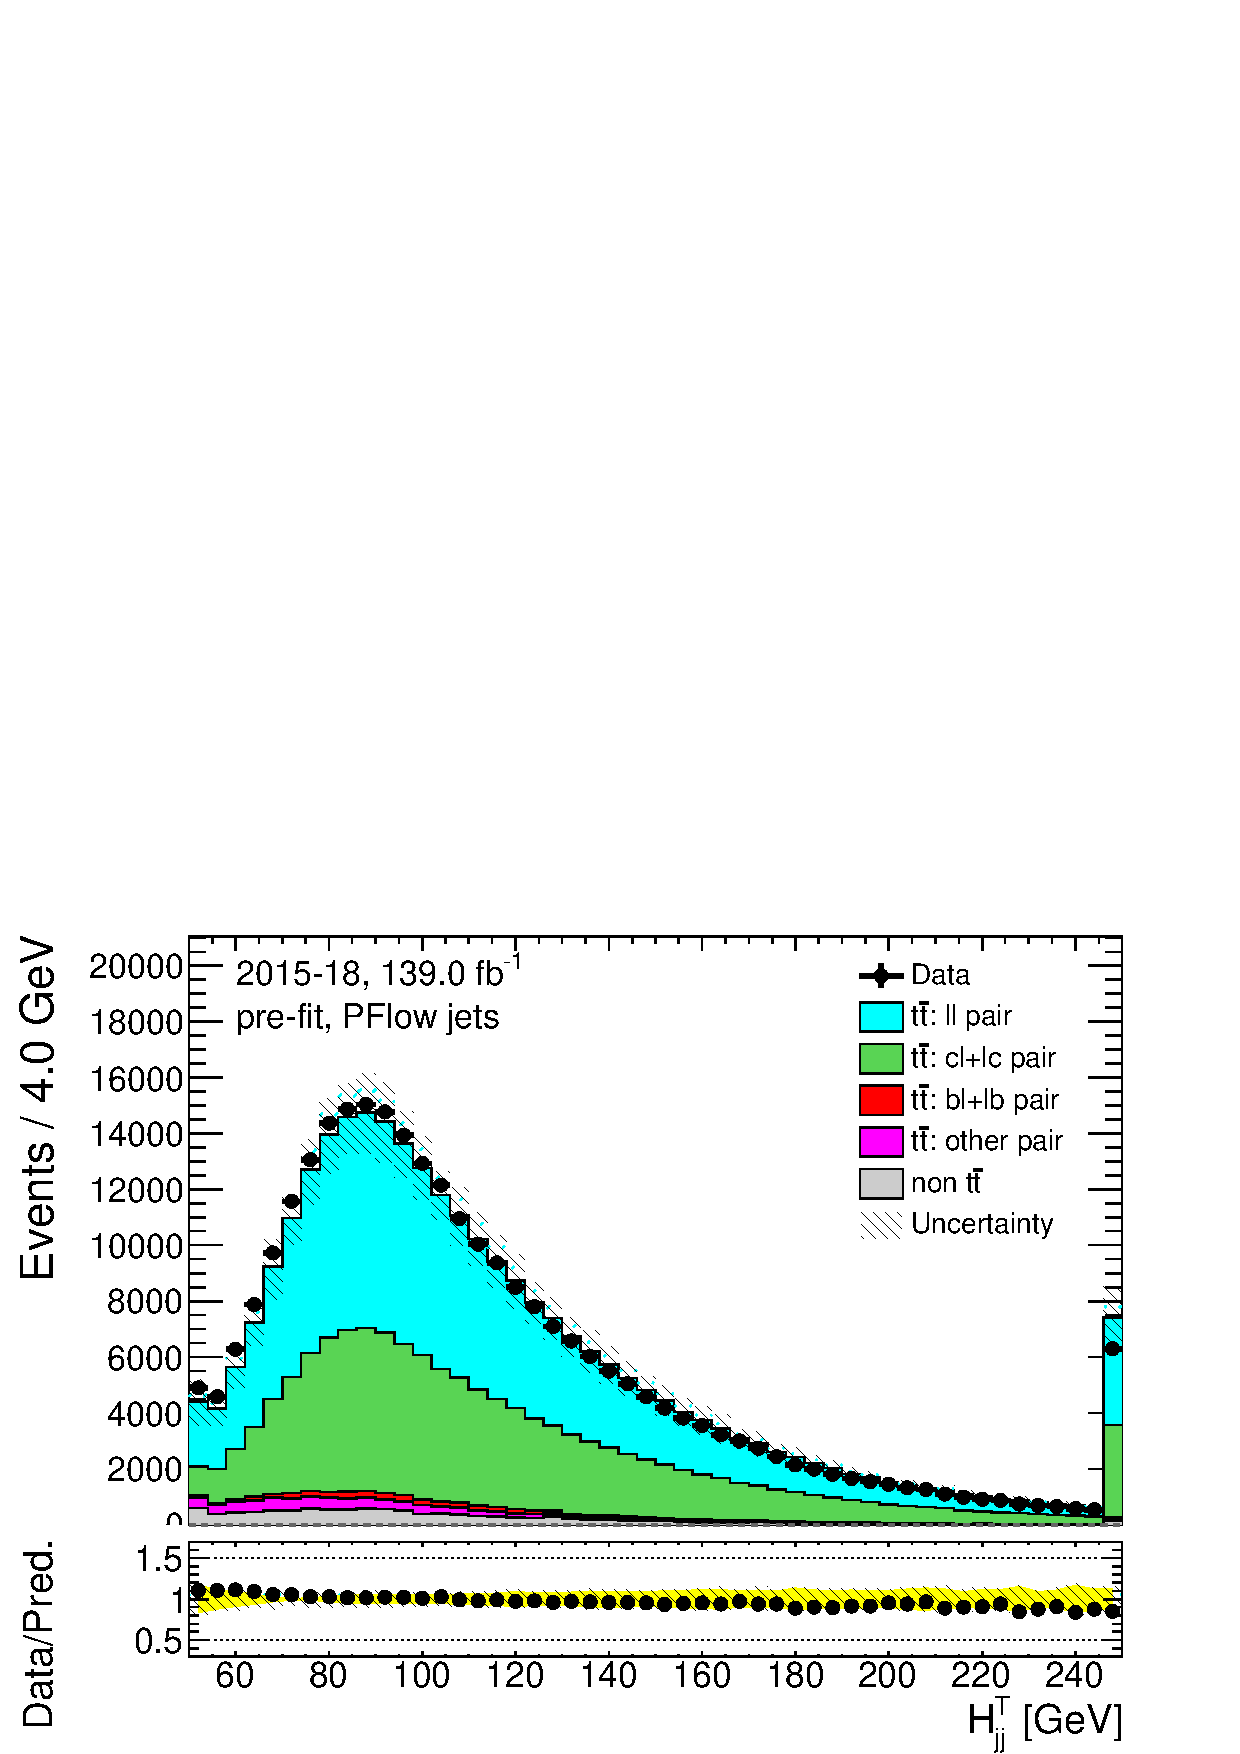
\includegraphics[width=.45\textwidth]{FTAG_plots/pretagNoRwwithouthighpTPFlowall/DataMC_h_Htjj.png}\\
\caption{PFlow jets: distributions of mass related variables of the standard selection, 
before fitting or 
tagging with stat-only uncertainties.} \label{fig:standard_mass_PFlow}
\end{figure}



\newpage	
\begin{figure}[H]
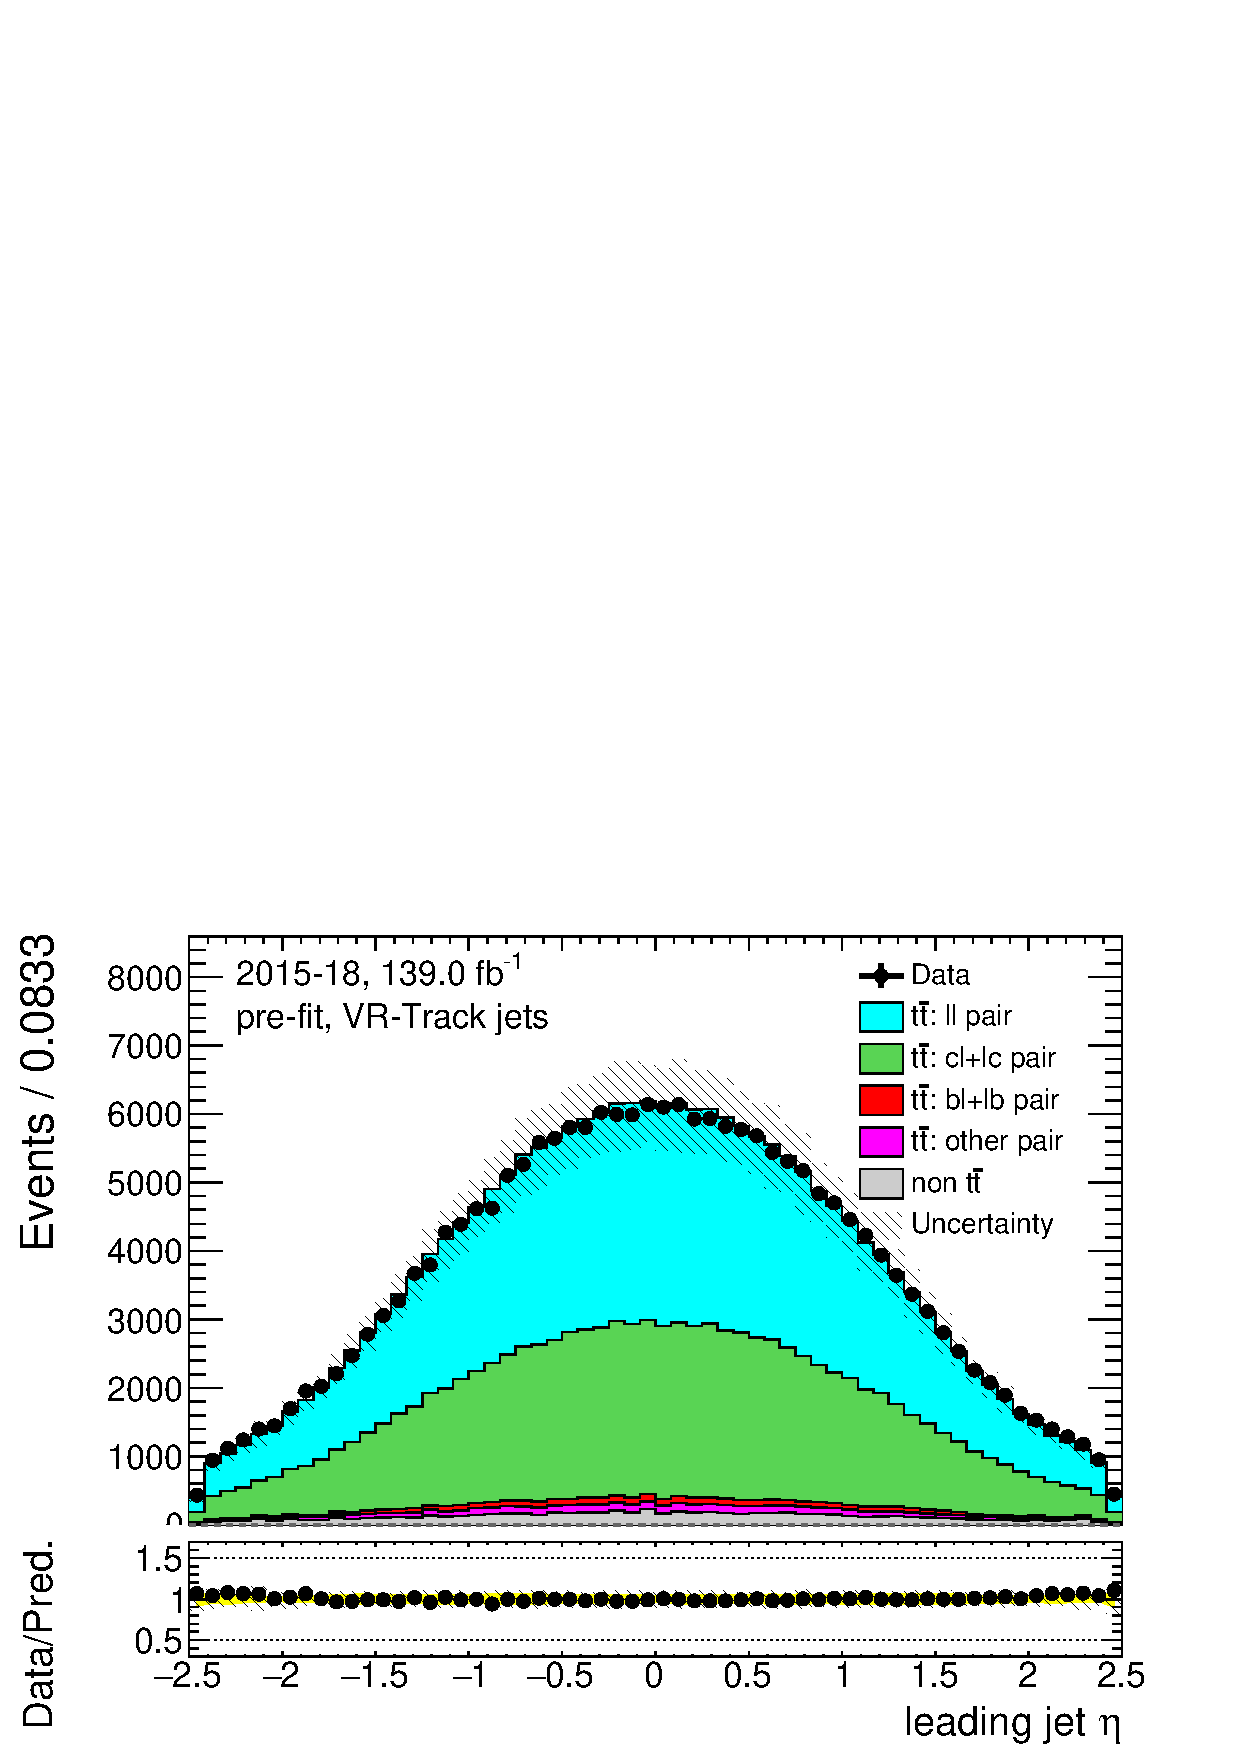
\includegraphics[width=.45\textwidth]{FTAG_plots/pretagNoRwwithouthighpTVRJetsall/DataMC_h_J0_etatrackjet.png}
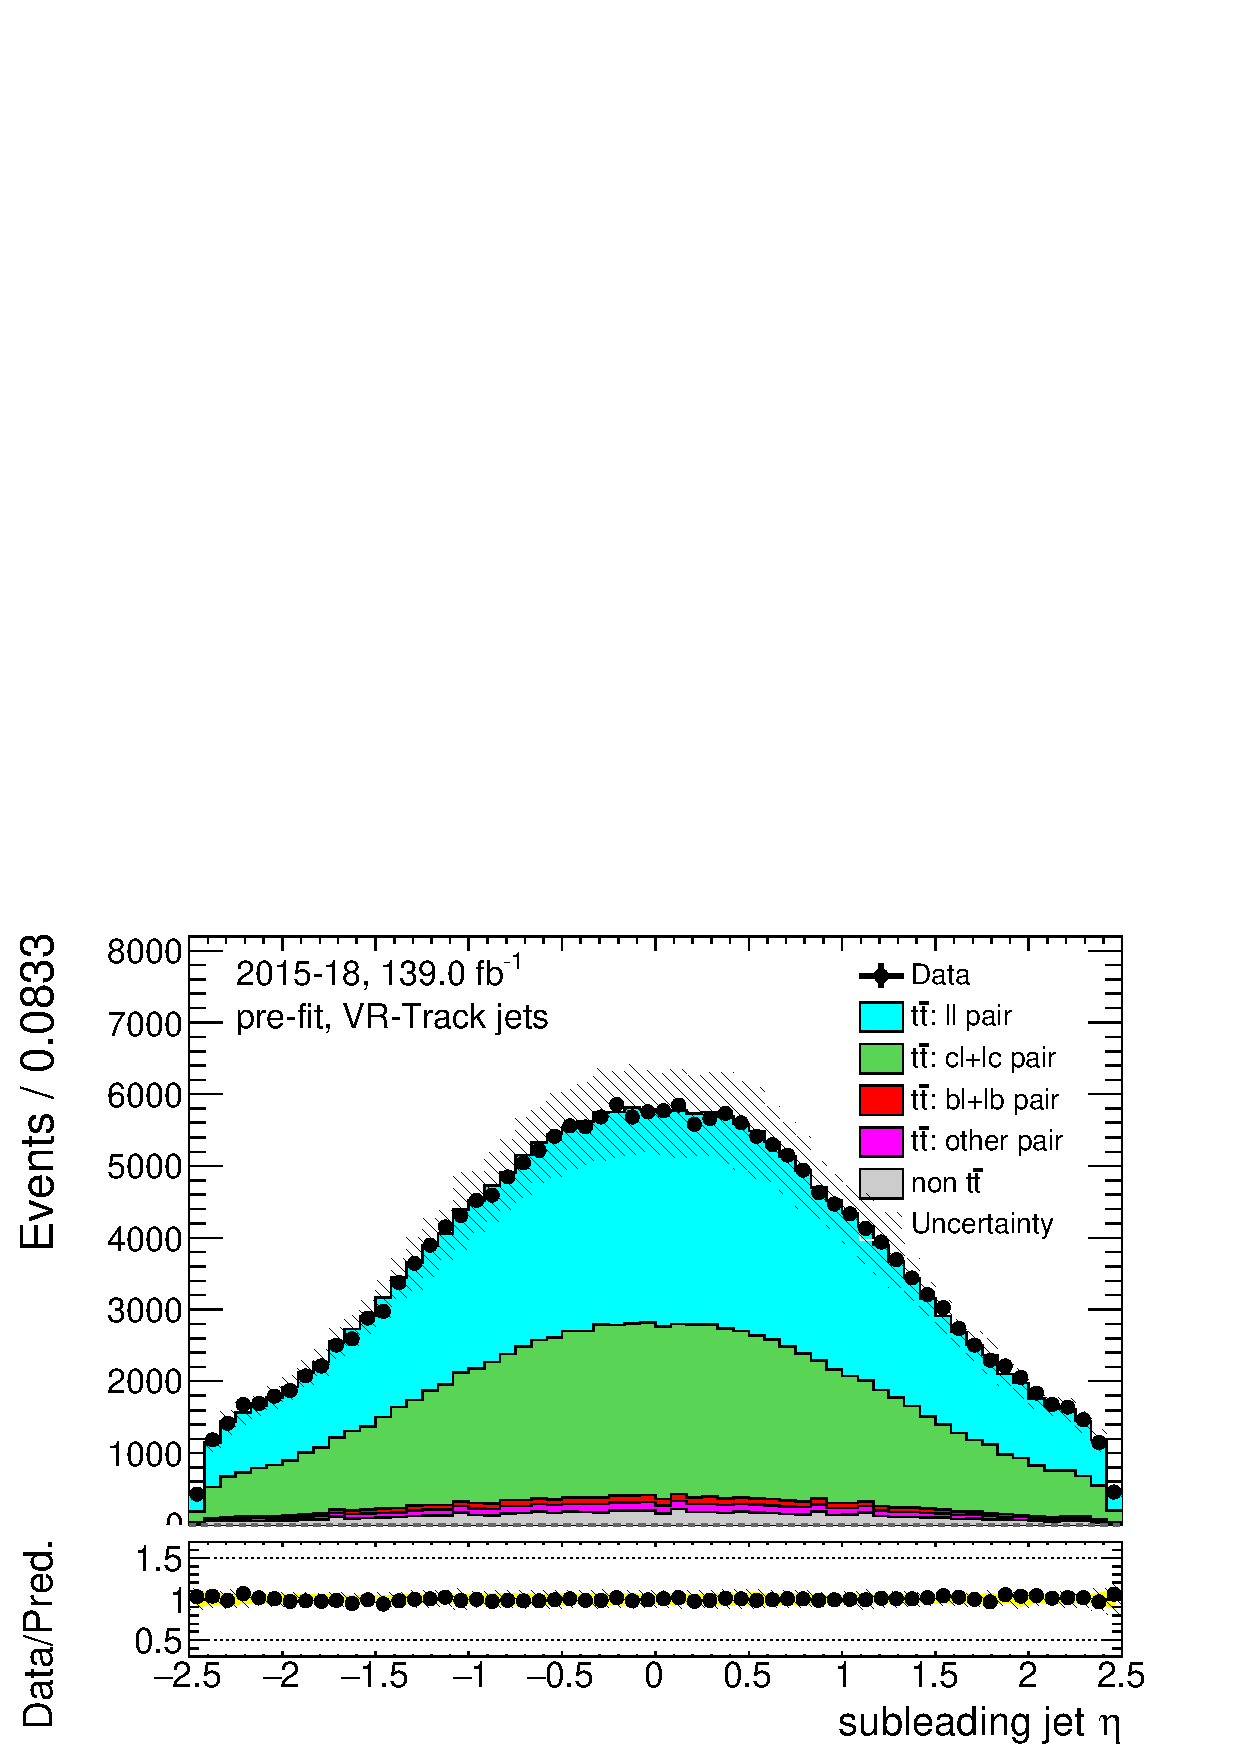
\includegraphics[width=.45\textwidth]{FTAG_plots/pretagNoRwwithouthighpTVRJetsall/DataMC_h_J1_etatrackjet.png}\\
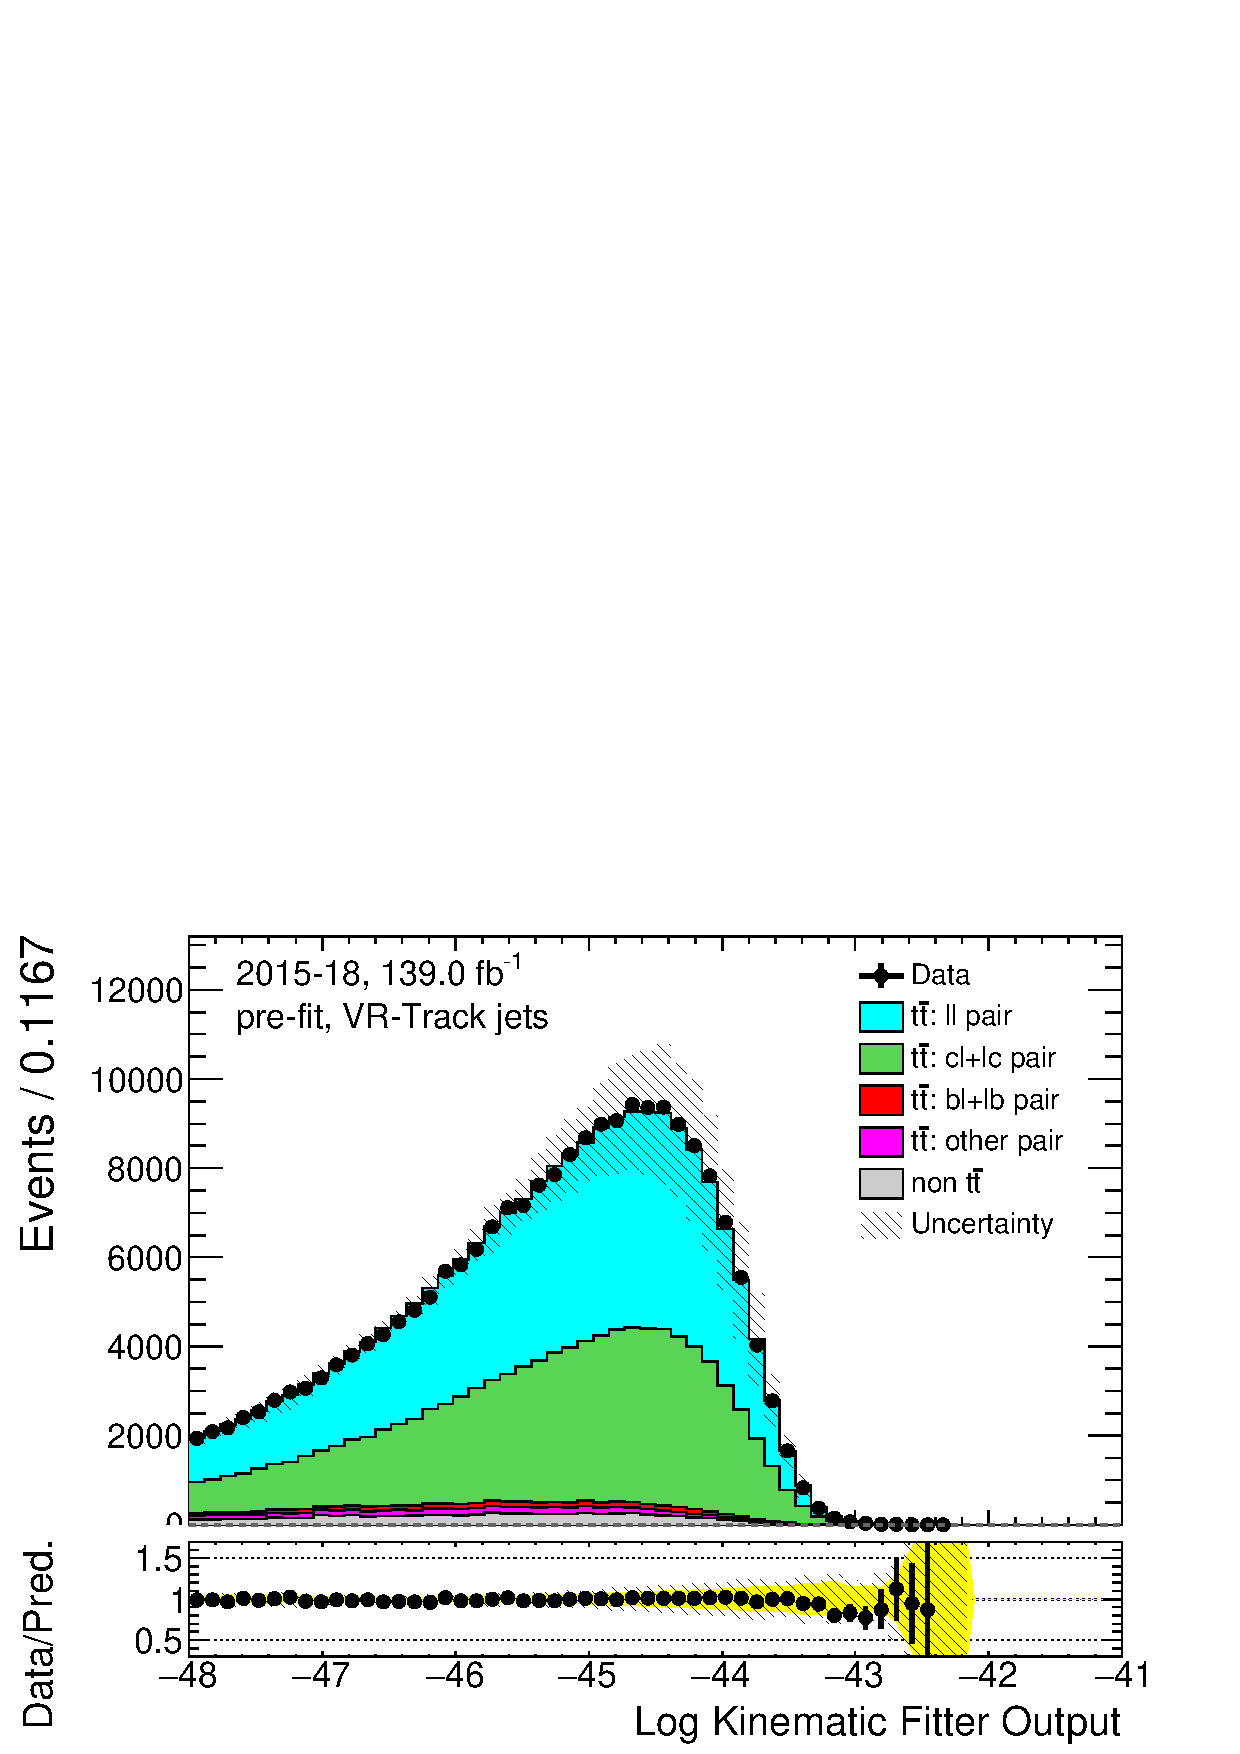
\includegraphics[width=.45\textwidth]{FTAG_plots/pretagNoRwwithouthighpTVRJetsall/DataMC_h_LLRtrackjet.png}
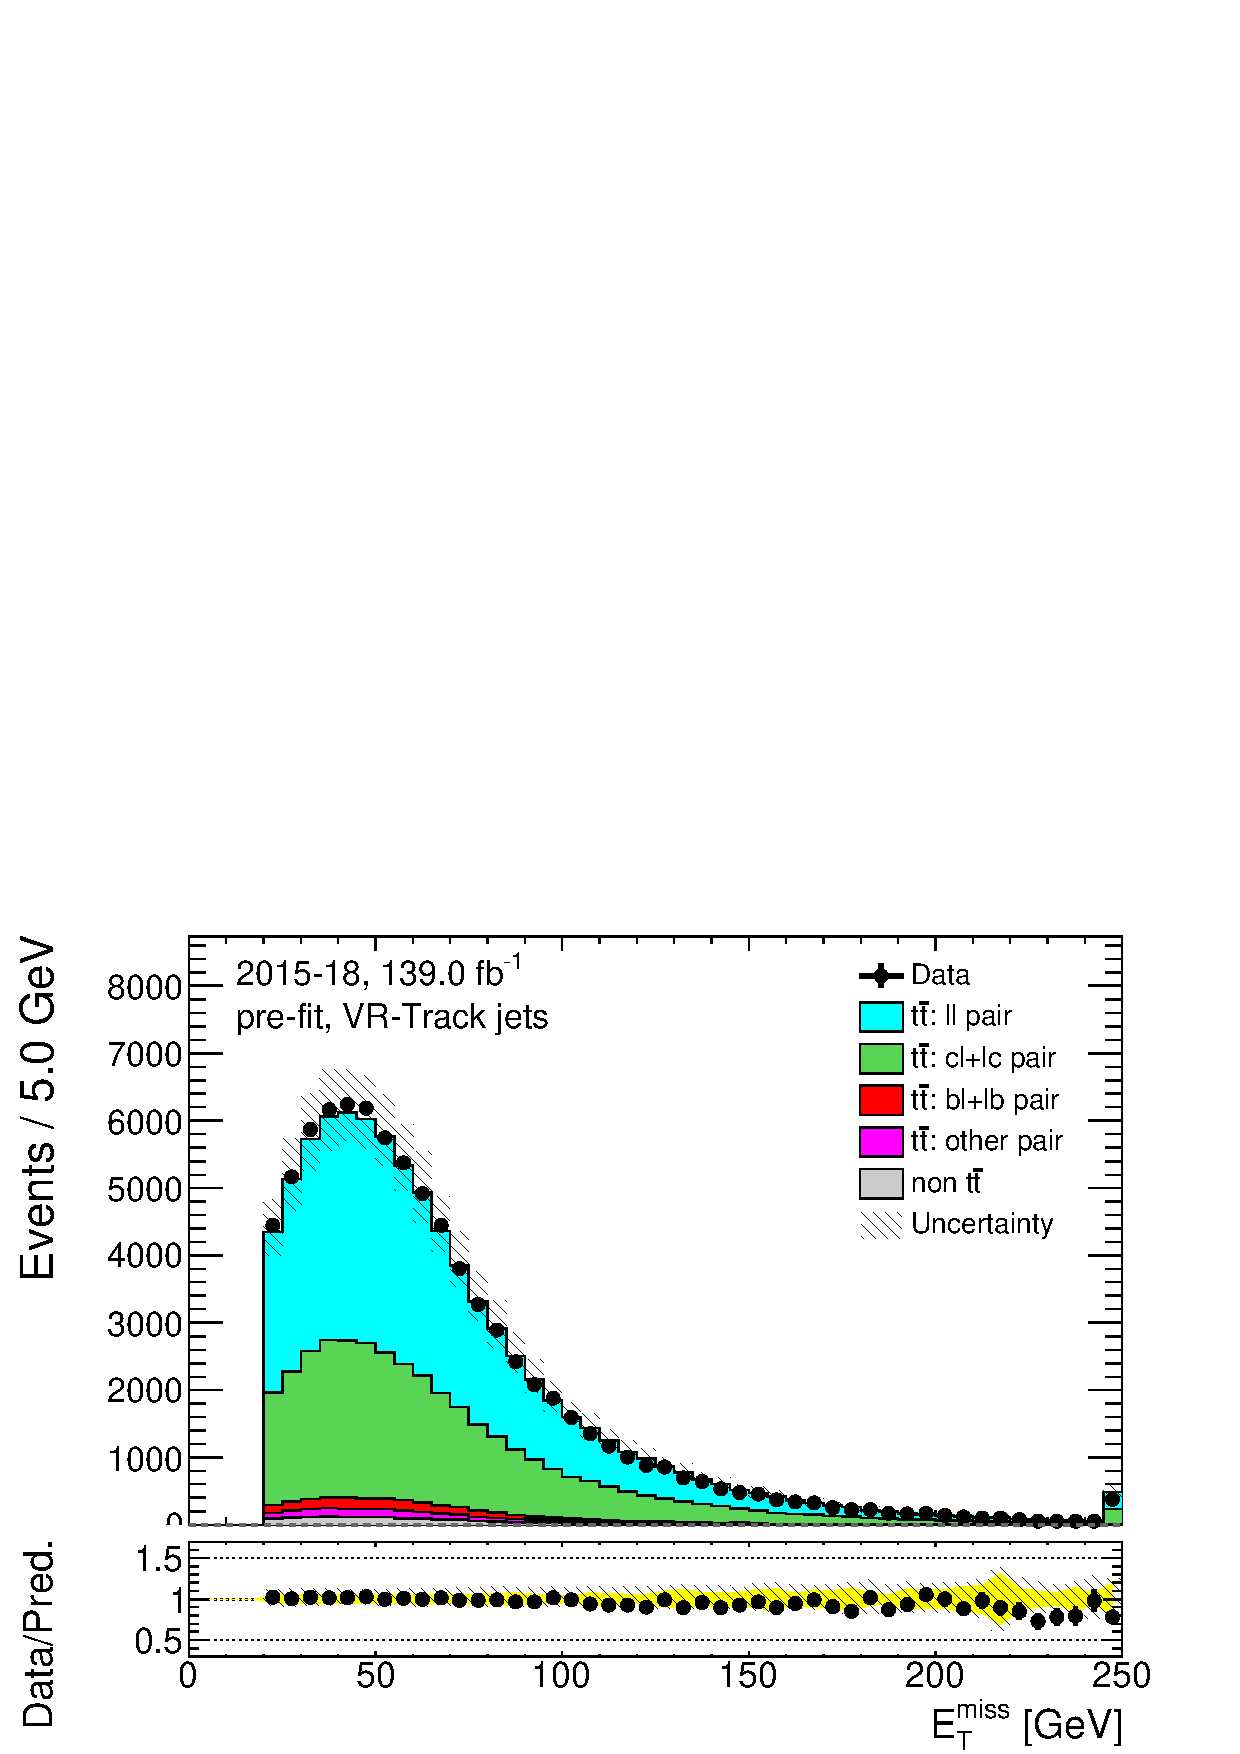
\includegraphics[width=.45\textwidth]{FTAG_plots/pretagNoRwwithouthighpTVRJetsall/DataMC_h_METtrackjet.png}\\

\caption{VR-Track jets: distributions of the leading and sub-leading jets 
from W decay, KLFitter output and the transverse missing transverse 
energy of the standard selection, before fitting or tagging with 
full uncertainties.} \label{fig:standard_jets_VRJets}
\end{figure}



\newpage
\begin{figure}[H]
\includegraphics[width=.45\textwidth]{FTAG_plots/pretagNoRwwithouthighpTVRJetsall/DataMC_h_dRbbtrackjet.png}
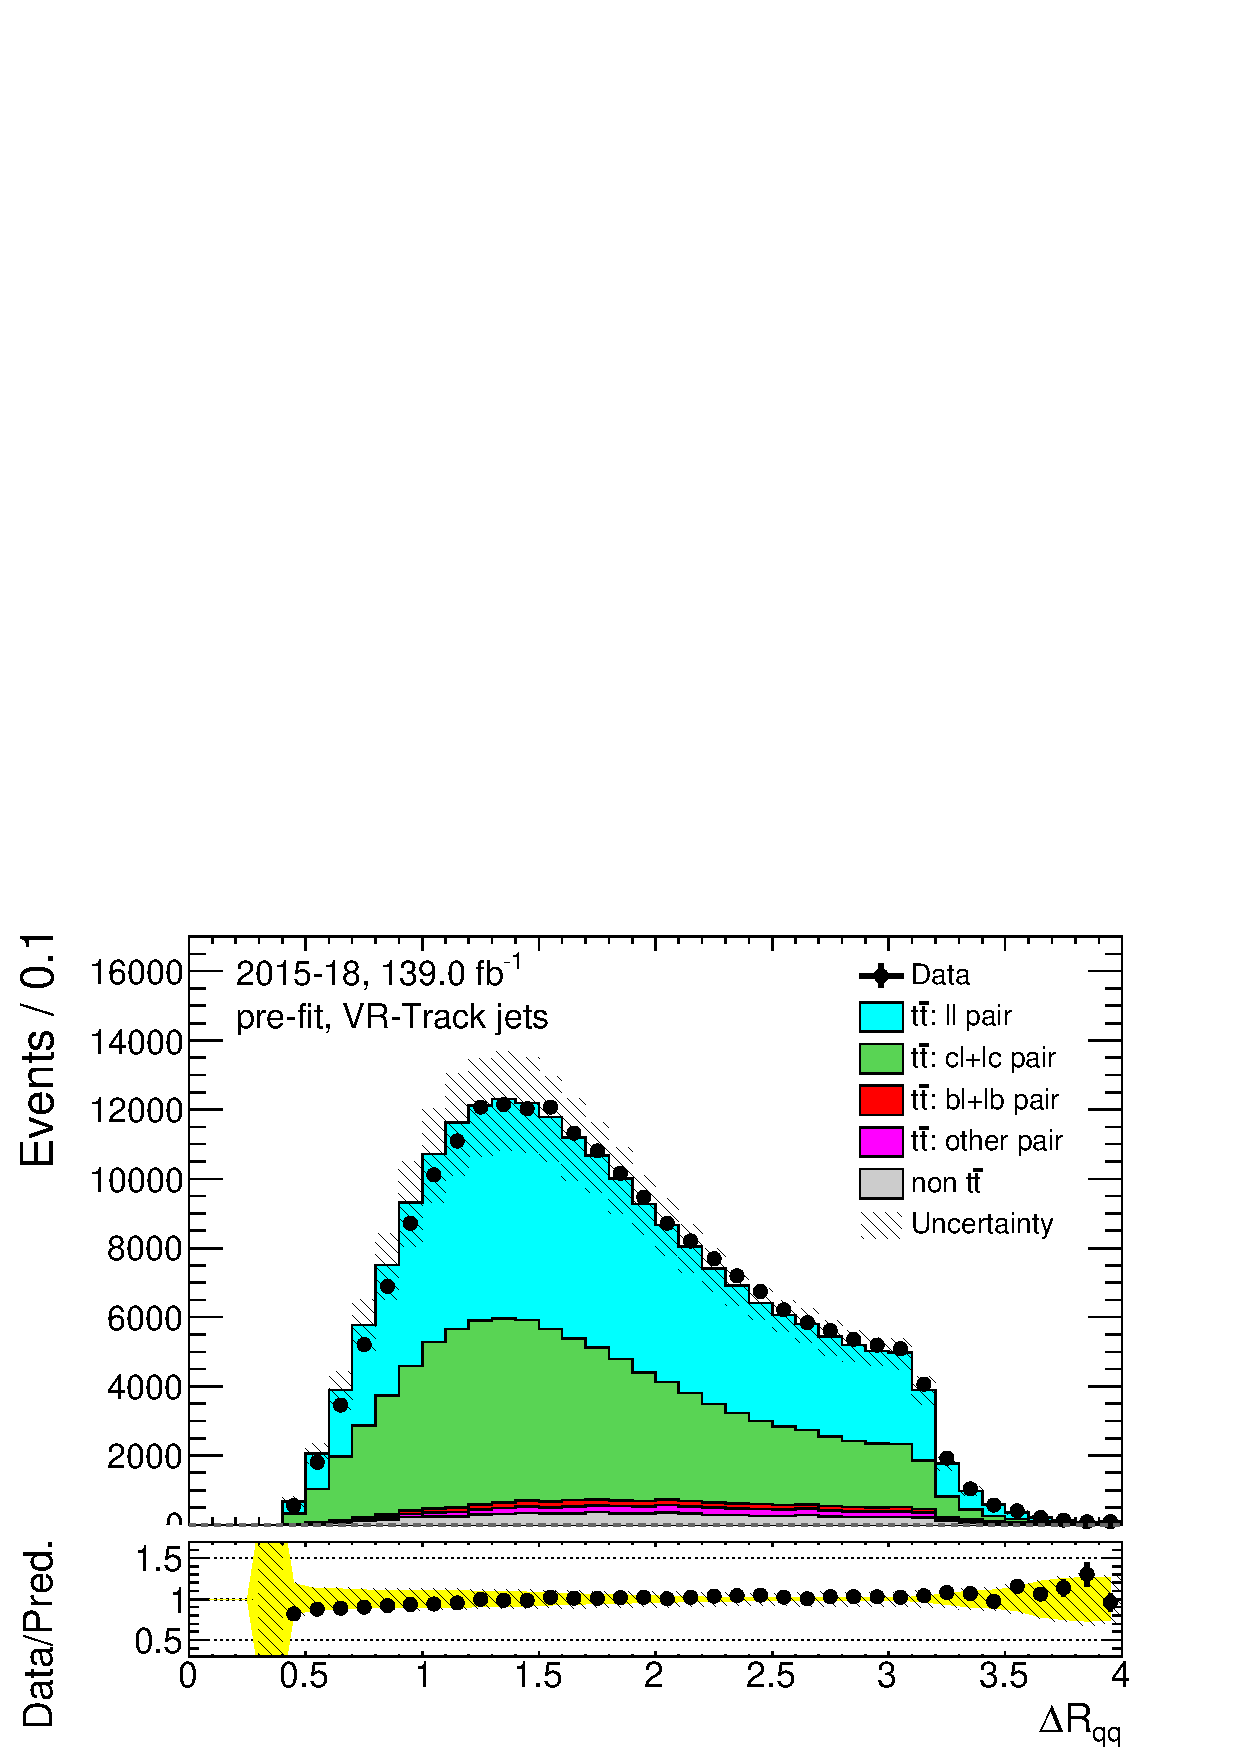
\includegraphics[width=.45\textwidth]{FTAG_plots/pretagNoRwwithouthighpTVRJetsall/DataMC_h_dRqqtrackjet.png}\\
\includegraphics[width=.45\textwidth]{FTAG_plots/pretagNoRwwithouthighpTVRJetsall/DataMC_h_dRbhadq1trackjet.png}
\includegraphics[width=.45\textwidth]{FTAG_plots/pretagNoRwwithouthighpTVRJetsall/DataMC_h_dRblepq1trackjet.png} \\
\includegraphics[width=.45\textwidth]{FTAG_plots/pretagNoRwwithouthighpTVRJetsall/DataMC_h_dRWhadbhadtrackjet.png} 
\includegraphics[width=.45\textwidth]{FTAG_plots/pretagNoRwwithouthighpTVRJetsall/DataMC_h_dRWhadbleptrackjet.png} \\
\caption{VR-Track jets: distributions of angle related variables of the combination 
of the standard selection, before fitting or tagging with full uncertainties.} \label{fig:standard_angles_VRJets}
\end{figure}

\newpage
\begin{figure}[H]
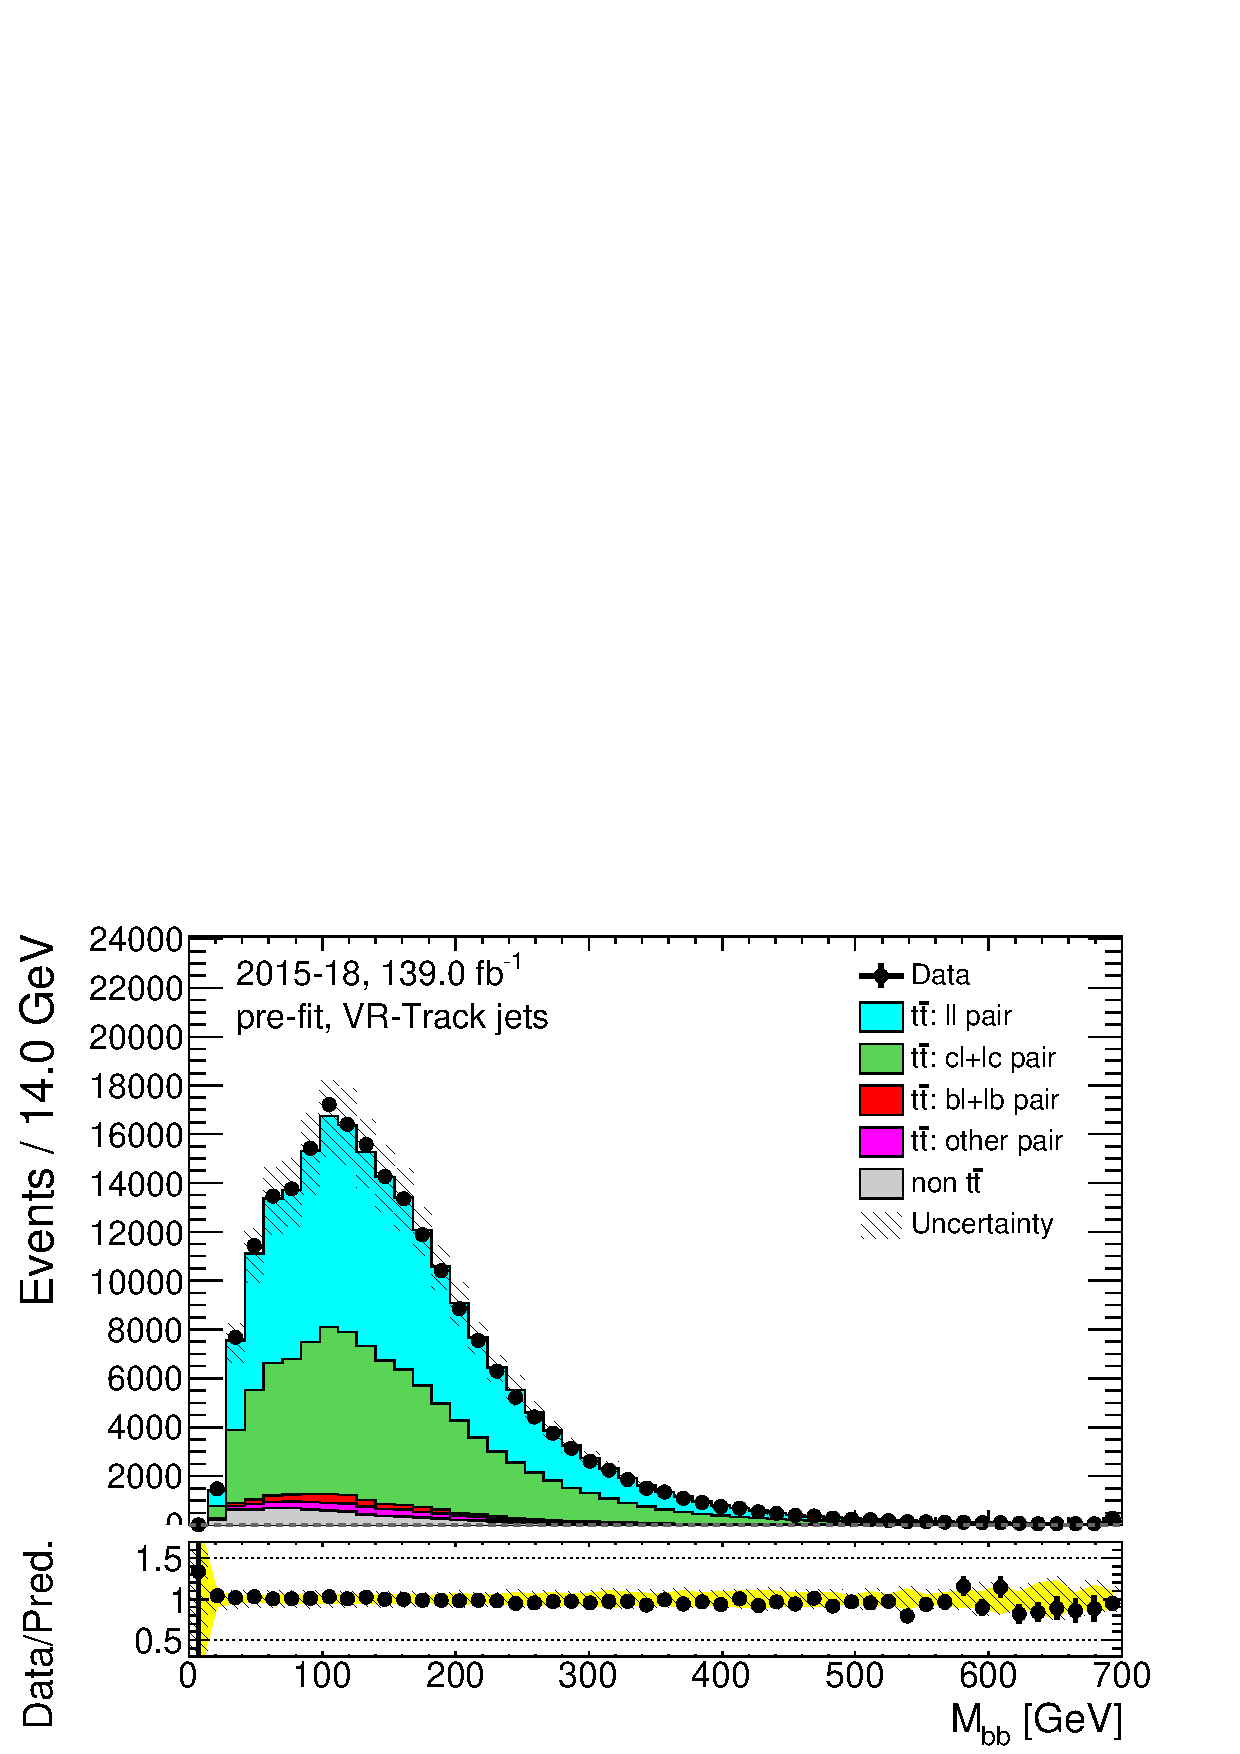
\includegraphics[width=.45\textwidth]{FTAG_plots/pretagNoRwwithouthighpTVRJetsall/DataMC_h_Mbbtrackjet.png}
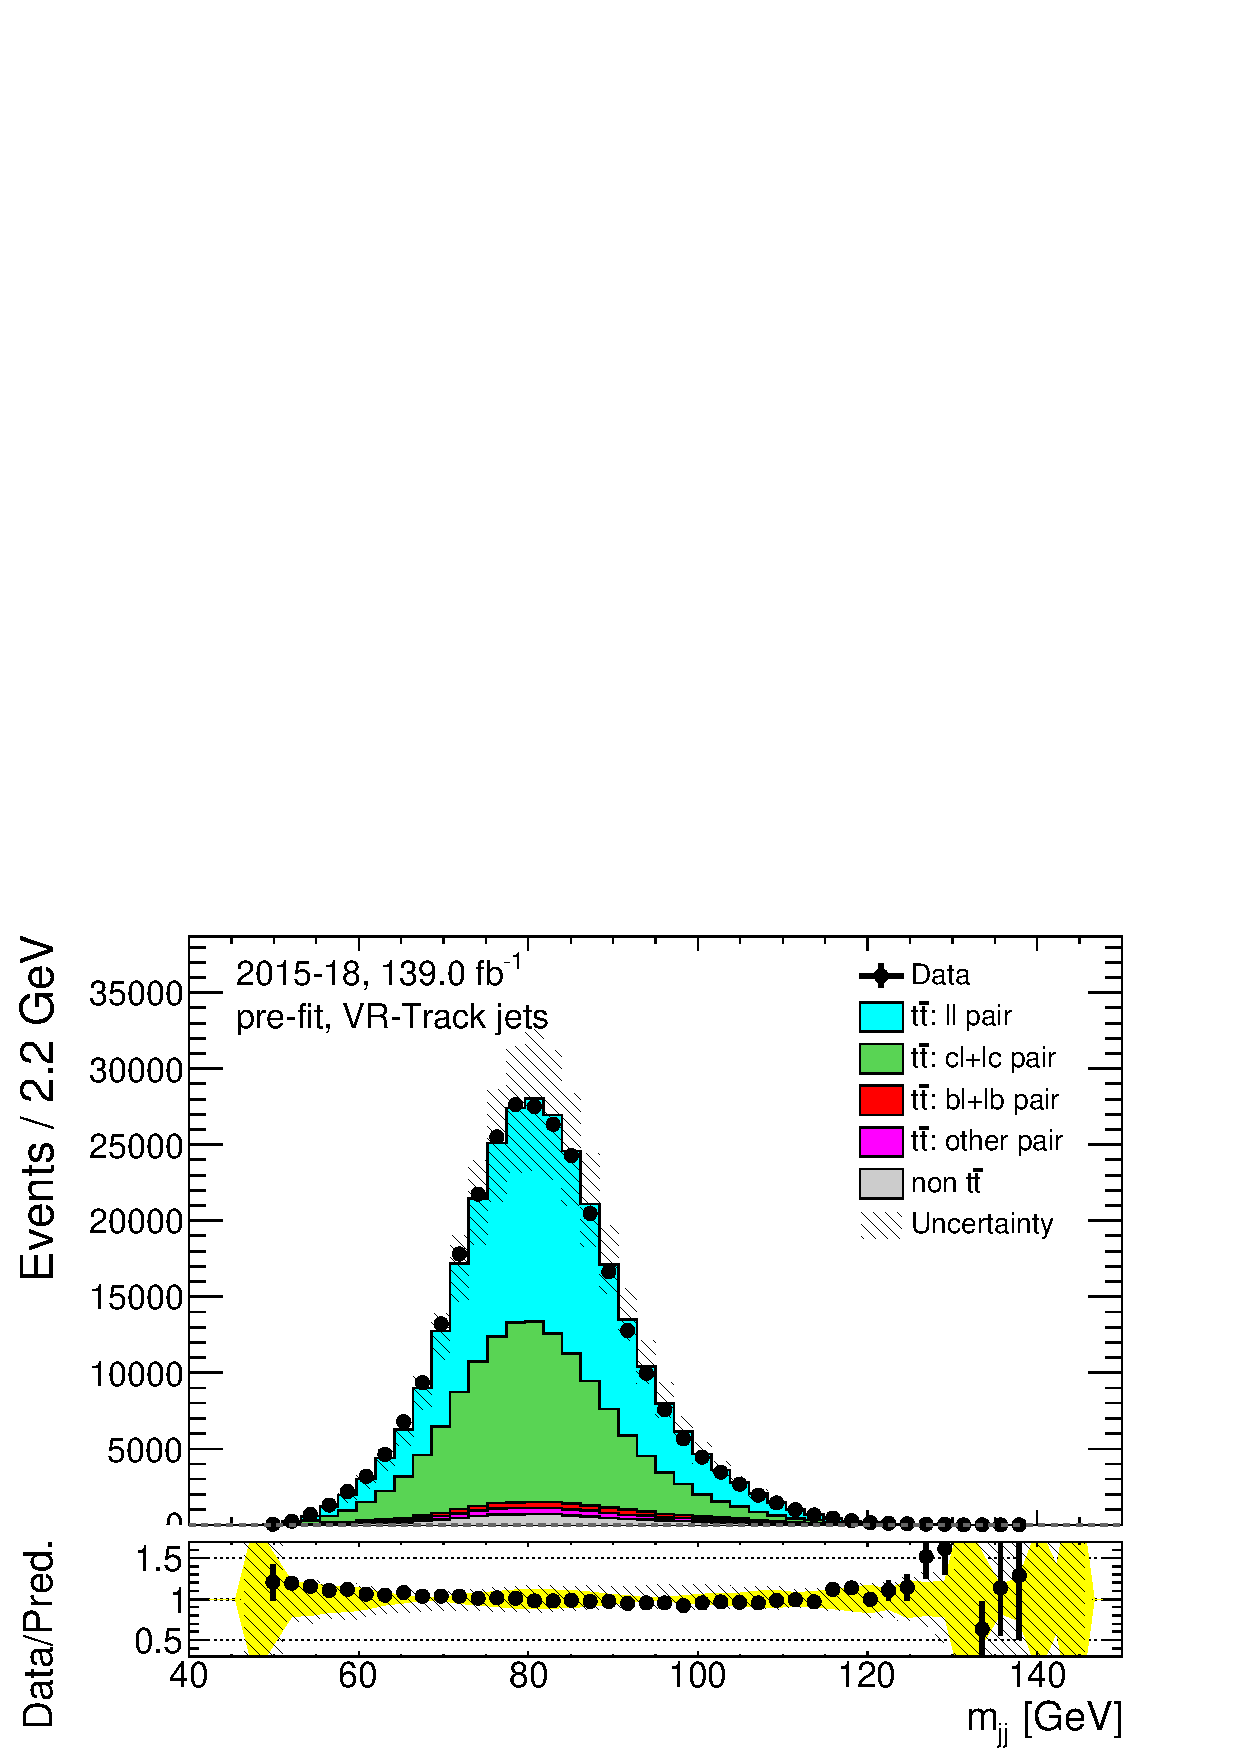
\includegraphics[width=.45\textwidth]{FTAG_plots/pretagNoRwwithouthighpTVRJetsall/DataMC_h_mjjtrackjet.png}\\
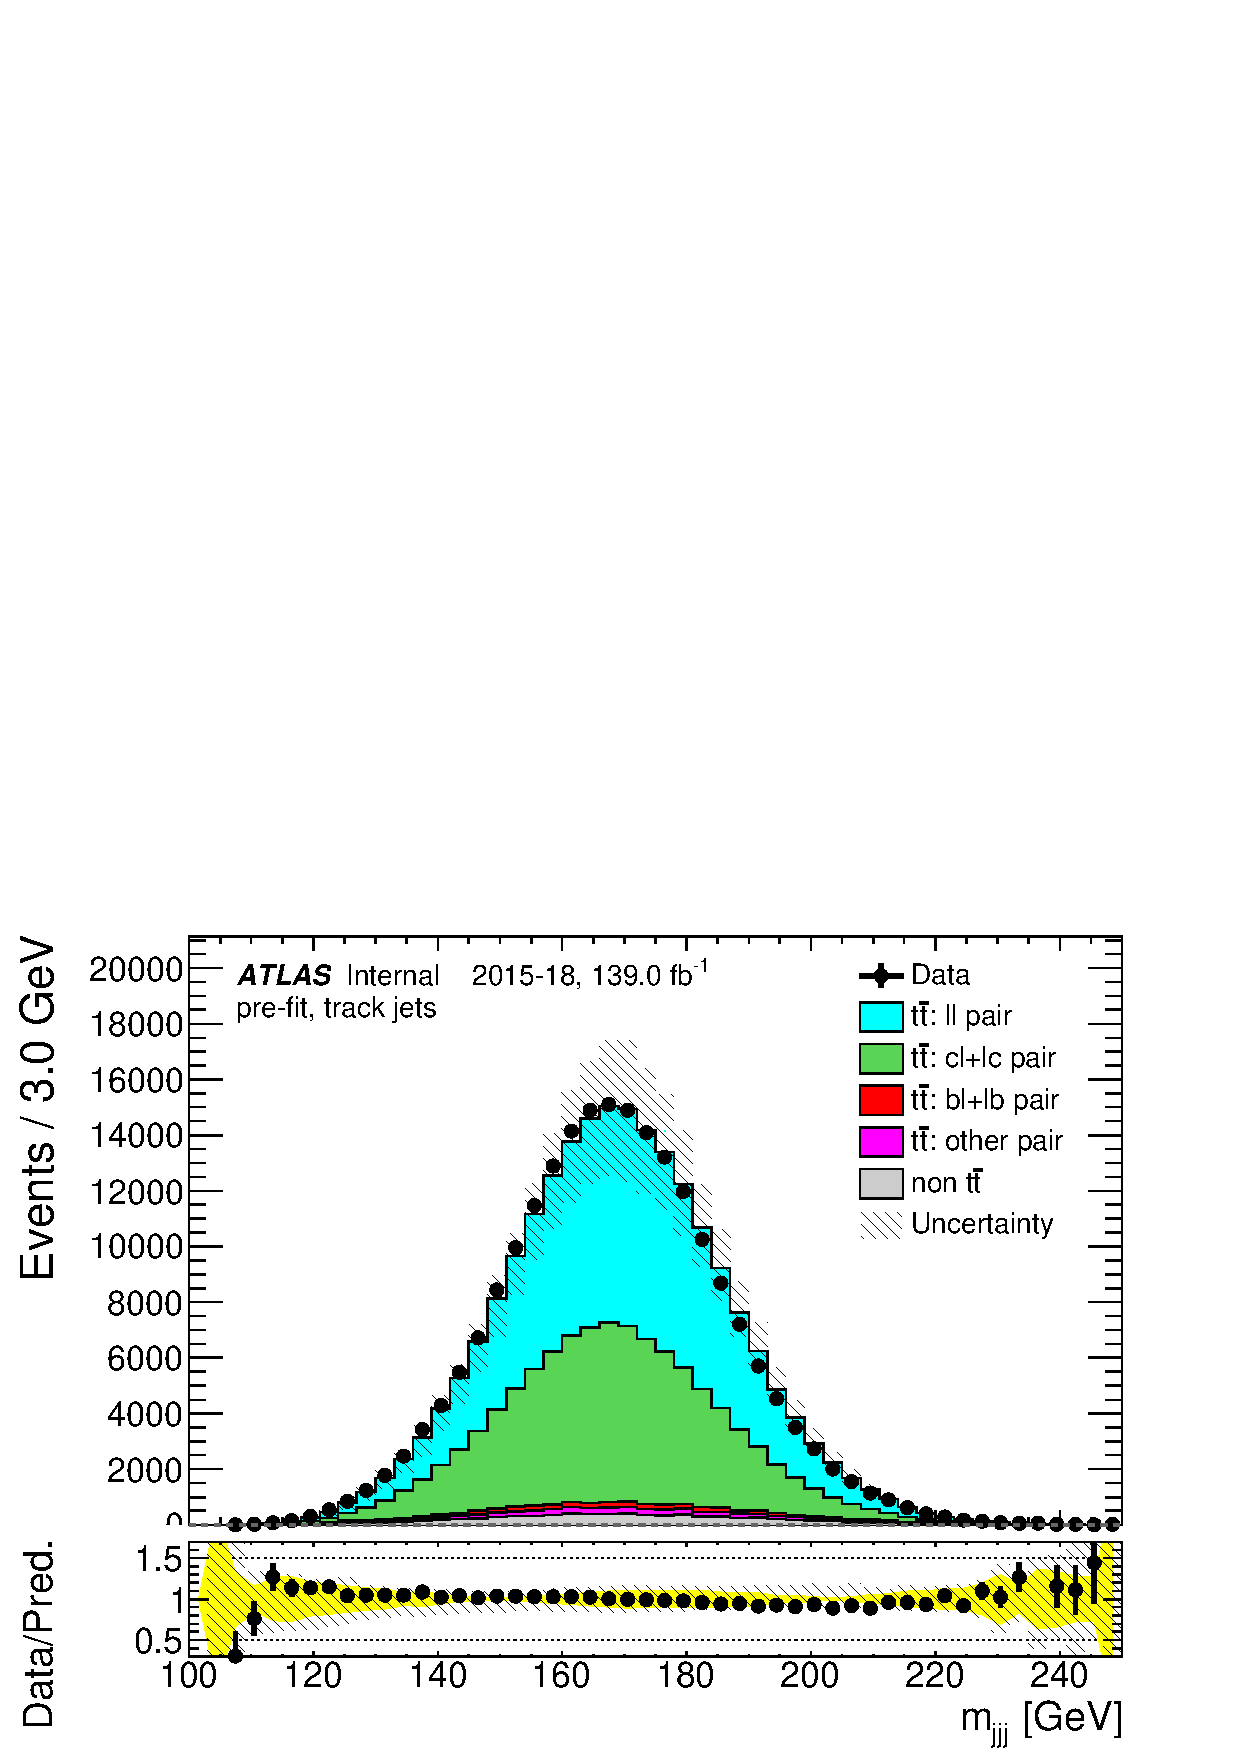
\includegraphics[width=.45\textwidth]{FTAG_plots/pretagNoRwwithouthighpTVRJetsall/DataMC_h_mjjjtrackjet.png}
\includegraphics[width=.45\textwidth]{FTAG_plots/pretagNoRwwithouthighpTVRJetsall/DataMC_h_Htjjtrackjet.png}\\
\caption{VR-Track jets: distributions of mass related variables of the standard selection, 
before fitting or tagging with stat-only uncertainties.} \label{fig:standard_mass_VRJets}
\end{figure}


\subsection{Low-\texorpdfstring{\pt}{pT} selection}
\label{sec:appendix_lowpT_selection}
\newpage	
\begin{figure}[H]
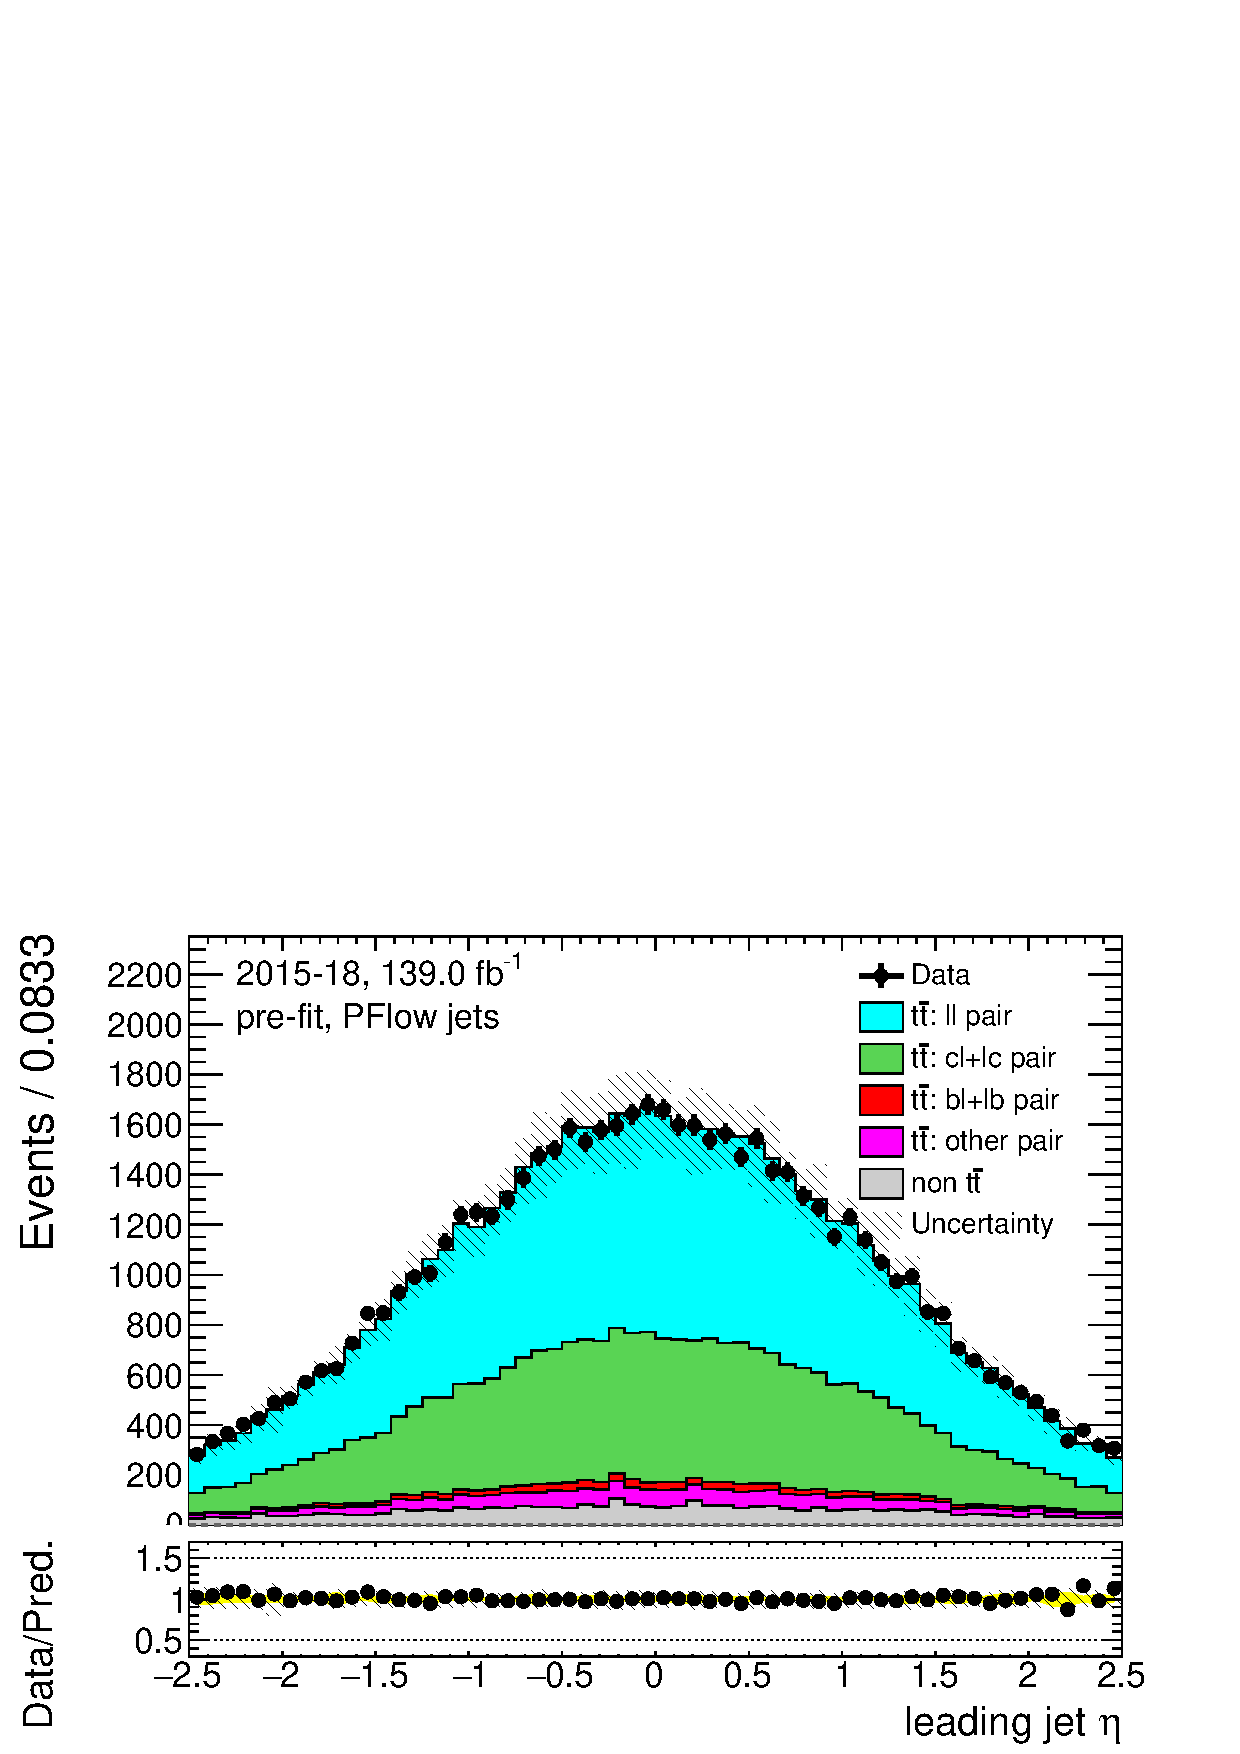
\includegraphics[width=.45\textwidth]{FTAG_plots/pretagNoRwLowpTPFlowall/DataMC_h_J0_eta.png}
\includegraphics[width=.45\textwidth]{FTAG_plots/pretagNoRwLowpTPFlowall/DataMC_h_J1_eta.png}\\
\includegraphics[width=.45\textwidth]{FTAG_plots/pretagNoRwLowpTPFlowall/DataMC_h_LLR.png}
\includegraphics[width=.45\textwidth]{FTAG_plots/pretagNoRwLowpTPFlowall/DataMC_h_MET.png}\\

\caption{PFlow jets: distributions of the leading and sub-leading jets 
from W decay, KLFitter output and the transverse missing transverse 
energy of the low-\pt\ selection, before fitting or tagging with 
full uncertainties.} \label{fig:lowpT_jets_VRJets}
\end{figure}

\newpage
\begin{figure}[H]
\includegraphics[width=.45\textwidth]{FTAG_plots/pretagNoRwLowpTPFlowall/DataMC_h_dRbb.png}
\includegraphics[width=.45\textwidth]{FTAG_plots/pretagNoRwLowpTPFlowall/DataMC_h_dRqq.png}\\
\includegraphics[width=.45\textwidth]{FTAG_plots/pretagNoRwLowpTPFlowall/DataMC_h_dRbhadq1.png}
\includegraphics[width=.45\textwidth]{FTAG_plots/pretagNoRwLowpTPFlowall/DataMC_h_dRblepq1.png} \\
\includegraphics[width=.45\textwidth]{FTAG_plots/pretagNoRwLowpTPFlowall/DataMC_h_dRWhadbhad.png} 
\includegraphics[width=.45\textwidth]{FTAG_plots/pretagNoRwLowpTPFlowall/DataMC_h_dRWhadblep.png} \\
\caption{PFlow jets: distributions of angle related variables of the combination of the low-\pt\ selection,
 before fitting or 
tagging with full uncertainties.} \label{fig:lowpT_angles_PFlow}
\end{figure}

\newpage
\begin{figure}[H]
\includegraphics[width=.45\textwidth]{FTAG_plots/pretagNoRwLowpTPFlowall/DataMC_h_Mbb.png}
\includegraphics[width=.45\textwidth]{FTAG_plots/pretagNoRwLowpTPFlowall/DataMC_h_mjj.png}\\
\includegraphics[width=.45\textwidth]{FTAG_plots/pretagNoRwLowpTPFlowall/DataMC_h_mjjj.png}
\includegraphics[width=.45\textwidth]{FTAG_plots/pretagNoRwLowpTPFlowall/DataMC_h_Htjj.png}\\
\caption{PFlow jets: distributions of mass related variables of the low-\pt\ selection, 
before fitting or 
tagging with stat-only uncertainties.} \label{fig:lowpT_mass_PFlow}
\end{figure}

\section{High-\texorpdfstring{\pt}{pT} selection}
\label{sec:appendix_highpT_selection}
\newpage	
\begin{figure}[H]
\includegraphics[width=.45\textwidth]{FTAG_plots/pretagNoRwnewonlyPFlowall/DataMC_h_J0_eta.png}
\includegraphics[width=.45\textwidth]{FTAG_plots/pretagNoRwnewonlyPFlowall/DataMC_h_J1_eta.png}\\
\includegraphics[width=.45\textwidth]{FTAG_plots/pretagNoRwnewonlyPFlowall/DataMC_h_LLR.png}
\includegraphics[width=.45\textwidth]{FTAG_plots/pretagNoRwnewonlyPFlowall/DataMC_h_MET.png}\\

\caption{PFlow jets: distributions of the leading and sub-leading jets 
from W decay, KLFitter output and the transverse missing transverse 
energy of the high-\pt\ selection, before fitting or tagging with 
full uncertainties.} \label{fig:highpT_jets_PFlow}
\end{figure}

\newpage
\begin{figure}[H]
\includegraphics[width=.45\textwidth]{FTAG_plots/pretagNoRwnewonlyPFlowall/DataMC_h_dRbb.png}
\includegraphics[width=.45\textwidth]{FTAG_plots/pretagNoRwnewonlyPFlowall/DataMC_h_dRqq.png}\\
\includegraphics[width=.45\textwidth]{FTAG_plots/pretagNoRwnewonlyPFlowall/DataMC_h_dRbhadq1.png}
\includegraphics[width=.45\textwidth]{FTAG_plots/pretagNoRwnewonlyPFlowall/DataMC_h_dRblepq1.png} \\
\includegraphics[width=.45\textwidth]{FTAG_plots/pretagNoRwnewonlyPFlowall/DataMC_h_dRWhadbhad.png} 
\includegraphics[width=.45\textwidth]{FTAG_plots/pretagNoRwnewonlyPFlowall/DataMC_h_dRWhadblep.png} \\
\caption{PFlow jets: distributions of angle related variables of the combination of the high-\pt\ selection,
 before fitting or 
tagging with full uncertainties.} \label{fig:highpT_angles_PFlow}
\end{figure}

\newpage
\begin{figure}[H]
\includegraphics[width=.45\textwidth]{FTAG_plots/pretagNoRwnewonlyPFlowall/DataMC_h_Mbb.png}
\includegraphics[width=.45\textwidth]{FTAG_plots/pretagNoRwnewonlyPFlowall/DataMC_h_mjj.png}\\
\includegraphics[width=.45\textwidth]{FTAG_plots/pretagNoRwnewonlyPFlowall/DataMC_h_mjjj.png}
\includegraphics[width=.45\textwidth]{FTAG_plots/pretagNoRwnewonlyPFlowall/DataMC_h_Htjj.png}\\
\caption{PFlow jets: distributions of mass related variables of the high-\pt\ selection, 
before fitting or 
tagging with stat-only uncertainties.} \label{fig:highpT_mass_PFlow}
\end{figure}



\newpage	
\begin{figure}[H]
\includegraphics[width=.45\textwidth]{FTAG_plots/pretagNoRwnewonlyVRJetsall/DataMC_h_J0_etatrackjet.png}
\includegraphics[width=.45\textwidth]{FTAG_plots/pretagNoRwnewonlyVRJetsall/DataMC_h_J1_etatrackjet.png}\\
\includegraphics[width=.45\textwidth]{FTAG_plots/pretagNoRwnewonlyVRJetsall/DataMC_h_LLRtrackjet.png}
\includegraphics[width=.45\textwidth]{FTAG_plots/pretagNoRwnewonlyVRJetsall/DataMC_h_METtrackjet.png}\\

\caption{VR-Track jets: distributions of the leading and sub-leading jets 
from W decay, KLFitter output and the transverse missing transverse 
energy of the high-\pt\ selection, before fitting or tagging with 
full uncertainties.} \label{fig:highpT_jets_VRJets}
\end{figure}



\newpage
\begin{figure}[H]
\includegraphics[width=.45\textwidth]{FTAG_plots/pretagNoRwnewonlyVRJetsall/DataMC_h_dRbbtrackjet.png}
\includegraphics[width=.45\textwidth]{FTAG_plots/pretagNoRwnewonlyVRJetsall/DataMC_h_dRqqtrackjet.png}\\
\includegraphics[width=.45\textwidth]{FTAG_plots/pretagNoRwnewonlyVRJetsall/DataMC_h_dRbhadq1trackjet.png}
\includegraphics[width=.45\textwidth]{FTAG_plots/pretagNoRwnewonlyVRJetsall/DataMC_h_dRblepq1trackjet.png} \\
\includegraphics[width=.45\textwidth]{FTAG_plots/pretagNoRwnewonlyVRJetsall/DataMC_h_dRWhadbhadtrackjet.png} 
\includegraphics[width=.45\textwidth]{FTAG_plots/pretagNoRwnewonlyVRJetsall/DataMC_h_dRWhadbleptrackjet.png} \\
\caption{VR-Track jets: distributions of angle related variables of the combination 
of the high-\pt\ selection, before fitting or tagging with full uncertainties.} \label{fig:highpT_angles_VRJets}
\end{figure}

\newpage
\begin{figure}[H]
\includegraphics[width=.45\textwidth]{FTAG_plots/pretagNoRwnewonlyVRJetsall/DataMC_h_Mbbtrackjet.png}
\includegraphics[width=.45\textwidth]{FTAG_plots/pretagNoRwnewonlyVRJetsall/DataMC_h_mjjtrackjet.png}\\
\includegraphics[width=.45\textwidth]{FTAG_plots/pretagNoRwnewonlyVRJetsall/DataMC_h_mjjjtrackjet.png}
\includegraphics[width=.45\textwidth]{FTAG_plots/pretagNoRwnewonlyVRJetsall/DataMC_h_Htjjtrackjet.png}\\
\caption{VR-Track jets: distributions of mass related variables of the high-\pt\ selection, 
before fitting or tagging with stat-only uncertainties.} \label{fig:highpT_mass_VRJets}
\end{figure}


	

	\newpage
	\section{Combined selection}
	\label{sec:appendix_combined_selection}
	\newpage	
	\begin{figure}[H]
	\includegraphics[width=.45\textwidth]{FTAG_plots/pretagNoRwwithhighpTPFlowall/DataMC_h_J0_eta.png}
	\includegraphics[width=.45\textwidth]{FTAG_plots/pretagNoRwwithhighpTPFlowall/DataMC_h_J1_eta.png}\\
	\includegraphics[width=.45\textwidth]{FTAG_plots/pretagNoRwwithhighpTPFlowall/DataMC_h_LLR.png}
	\includegraphics[width=.45\textwidth]{FTAG_plots/pretagNoRwwithhighpTPFlowall/DataMC_h_MET.png}\\
	
	\caption{PFlow jets: distributions of the leading and sub-leading jets 
	from W decay, KLFitter output and the transverse missing transverse 
	energy of the combined selection, before fitting or tagging with 
	full uncertainties.} \label{fig:combined_jets_PFlow}
	\end{figure}
	
	\newpage
	\begin{figure}[H]
	\includegraphics[width=.45\textwidth]{FTAG_plots/pretagNoRwwithhighpTPFlowall/DataMC_h_dRbb.png}
	\includegraphics[width=.45\textwidth]{FTAG_plots/pretagNoRwwithhighpTPFlowall/DataMC_h_dRqq.png}\\
	\includegraphics[width=.45\textwidth]{FTAG_plots/pretagNoRwwithhighpTPFlowall/DataMC_h_dRbhadq1.png}
	\includegraphics[width=.45\textwidth]{FTAG_plots/pretagNoRwwithhighpTPFlowall/DataMC_h_dRblepq1.png} \\
	\includegraphics[width=.45\textwidth]{FTAG_plots/pretagNoRwwithhighpTPFlowall/DataMC_h_dRWhadbhad.png} 
	\includegraphics[width=.45\textwidth]{FTAG_plots/pretagNoRwwithhighpTPFlowall/DataMC_h_dRWhadblep.png} \\
	\caption{PFlow jets: distributions of angle related variables of the combination of the combined selection,
	 before fitting or 
	tagging with full uncertainties.} \label{fig:combined_angles_PFlow}
	\end{figure}
	
	\newpage
	\begin{figure}[H]
	\includegraphics[width=.45\textwidth]{FTAG_plots/pretagNoRwwithhighpTPFlowall/DataMC_h_Mbb.png}
	\includegraphics[width=.45\textwidth]{FTAG_plots/pretagNoRwwithhighpTPFlowall/DataMC_h_mjj.png}\\
	\includegraphics[width=.45\textwidth]{FTAG_plots/pretagNoRwwithhighpTPFlowall/DataMC_h_mjjj.png}
	\includegraphics[width=.45\textwidth]{FTAG_plots/pretagNoRwwithhighpTPFlowall/DataMC_h_Htjj.png}\\
	\caption{PFlow jets: distributions of mass related variables of the combined selection, 
	before fitting or 
	tagging with stat-only uncertainties.} \label{fig:combined_mass_PFlow}
	\end{figure}
	
	
	
	\newpage	
	\begin{figure}[H]
	\includegraphics[width=.45\textwidth]{FTAG_plots/pretagNoRwwithhighpTVRJetsall/DataMC_h_J0_etatrackjet.png}
	\includegraphics[width=.45\textwidth]{FTAG_plots/pretagNoRwwithhighpTVRJetsall/DataMC_h_J1_etatrackjet.png}\\
	\includegraphics[width=.45\textwidth]{FTAG_plots/pretagNoRwwithhighpTVRJetsall/DataMC_h_LLRtrackjet.png}
	\includegraphics[width=.45\textwidth]{FTAG_plots/pretagNoRwwithhighpTVRJetsall/DataMC_h_METtrackjet.png}\\
	
	\caption{VR-Track jets: distributions of the leading and sub-leading jets 
	from W decay, KLFitter output and the transverse missing transverse 
	energy of the combined selection, before fitting or tagging with 
	full uncertainties.} \label{fig:combined_jets_VRJets}
	\end{figure}
	
	
	
	\newpage
	\begin{figure}[H]
	\includegraphics[width=.45\textwidth]{FTAG_plots/pretagNoRwwithhighpTVRJetsall/DataMC_h_dRbbtrackjet.png}
	\includegraphics[width=.45\textwidth]{FTAG_plots/pretagNoRwwithhighpTVRJetsall/DataMC_h_dRqqtrackjet.png}\\
	\includegraphics[width=.45\textwidth]{FTAG_plots/pretagNoRwwithhighpTVRJetsall/DataMC_h_dRbhadq1trackjet.png}
	\includegraphics[width=.45\textwidth]{FTAG_plots/pretagNoRwwithhighpTVRJetsall/DataMC_h_dRblepq1trackjet.png} \\
	\includegraphics[width=.45\textwidth]{FTAG_plots/pretagNoRwwithhighpTVRJetsall/DataMC_h_dRWhadbhadtrackjet.png} 
	\includegraphics[width=.45\textwidth]{FTAG_plots/pretagNoRwwithhighpTVRJetsall/DataMC_h_dRWhadbleptrackjet.png} \\
	\caption{VR-Track jets: distributions of angle related variables of the combination 
	of the combined selection, before fitting or tagging with full uncertainties.} \label{fig:combined_angles_VRJets}
	\end{figure}
	
	\newpage
	\begin{figure}[H]
	\includegraphics[width=.45\textwidth]{FTAG_plots/pretagNoRwwithhighpTVRJetsall/DataMC_h_Mbbtrackjet.png}
	\includegraphics[width=.45\textwidth]{FTAG_plots/pretagNoRwwithhighpTVRJetsall/DataMC_h_mjjtrackjet.png}\\
	\includegraphics[width=.45\textwidth]{FTAG_plots/pretagNoRwwithhighpTVRJetsall/DataMC_h_mjjjtrackjet.png}
	\includegraphics[width=.45\textwidth]{FTAG_plots/pretagNoRwwithhighpTVRJetsall/DataMC_h_Htjjtrackjet.png}\\
	\caption{VR-Track jets: distributions of mass related variables of the combined selection, 
	before fitting or tagging with stat-only uncertainties.} \label{fig:combined_mass_VRJets}
	\end{figure}
	
	

% \section{Plots for previous calibrations}



% \newpage
% \begin{figure}[H]
% \includegraphics[width=1\textwidth]{Dec_eff.png}
% \caption{Calibration of derivation p3970 in December 2019, given for  4 different working points.}\label{fig:Dec_eff}
% \end{figure}
% \newpage
% \begin{figure}[H]
% \includegraphics[width=1\textwidth]{Dec.png}
% \caption{Calibration result of derivation p3970 in December 2019, given for  4 different working points.}\label{fig:Dec}
% \end{figure}


\newpage
	

\section{Experimental uncertainties}








\begin{table}[H]
\begin{centering}
\begin{tabular}{p{25em}}

          \hline
          \textbf{Systematic uncertainty}
          \\
          \hline
          \hline
        EG\_RESOLUTION\_ALL
        \\
		\hline
		MUON\_ID
		\\
		MUON\_MS
		\\
		\hline
		MET\_SoftTrk\_ResoPara
		\\
		MET\_SoftTrk\_ResoPerp
		\\
		MET\_SoftTrk\_ScaleDown
		\\
		MET\_SoftTrk\_ScaleUp
		\\
		\hline
		JET\_Pileup\_OffsetNPV
		\\
		JET\_Pileup\_RhoTopology
		\\
		\hline
		JET\_EffectiveNP\_Modelling1
		\\ 
		JET\_EffectiveNP\_Modelling2
		\\ 
		JET\_EffectiveNP\_Modelling3
		\\ 
		JET\_EffectiveNP\_Modelling4
		\\ 
		JET\_EffectiveNP\_Statistical4
		\\ 
		JET\_EffectiveNP\_Detector1
		\\ 
		\hline 
		JET\_JER\_EffectiveNP\_1
		\\ 
		JET\_JER\_EffectiveNP\_2
		\\ 
		JET\_JER\_EffectiveNP\_3
		\\ 
		JET\_JER\_EffectiveNP\_4
		\\ 
		\hline 
		JET\_BJES\_Response
		\\ 
		\hline 
		JET\_Flavor\_Composition
		\\ 
		JET\_Flavor\_Response
        \\ 
        \hline

 \end{tabular} 
 
 \end{centering}
 \caption{List of experimental systematics.}\label{tab:systematics}
 \end{table}

\section{Search for Higgs boson pair production in the \bbtt\ channel}
\label{sec:search for dihiggs}
\subsection{Data and Monte Carlo samples}
\subsection{Trigger and event selection}
\subsection{Background estimation}
\subsection{Multivariate analysis}
\subsection{Systematic uncertainties}
\subsection{Results}
\section{Summary}

\printbibliography
\appendix

\chapter{Supplementary material for \texorpdfstring{\cjet}{c-jet} calibration}
\section{Additional plots for kinematic variables}
\subsection{Standard selection}

\label{sec:appendix_standard_selection}
\newpage	
\begin{figure}[H]
\includegraphics[width=.45\textwidth]{FTAG_plots/pretagNoRwwithouthighpTPFlowall/DataMC_h_J0_eta.png}
\includegraphics[width=.45\textwidth]{FTAG_plots/pretagNoRwwithouthighpTPFlowall/DataMC_h_J1_eta.png}\\
\includegraphics[width=.45\textwidth]{FTAG_plots/pretagNoRwwithouthighpTPFlowall/DataMC_h_LLR.png}
\includegraphics[width=.45\textwidth]{FTAG_plots/pretagNoRwwithouthighpTPFlowall/DataMC_h_MET.png}\\

\caption{PFlow jets: distributions of the leading and sub-leading jets 
from W decay, KLFitter output and the transverse missing transverse 
energy of the standard selection, before fitting or tagging with 
full uncertainties.} \label{fig:standard_jets_PFlow}
\end{figure}

\newpage
\begin{figure}[H]
\includegraphics[width=.45\textwidth]{FTAG_plots/pretagNoRwwithouthighpTPFlowall/DataMC_h_dRbb.png}
\includegraphics[width=.45\textwidth]{FTAG_plots/pretagNoRwwithouthighpTPFlowall/DataMC_h_dRqq.png}\\
\includegraphics[width=.45\textwidth]{FTAG_plots/pretagNoRwwithouthighpTPFlowall/DataMC_h_dRbhadq1.png}
\includegraphics[width=.45\textwidth]{FTAG_plots/pretagNoRwwithouthighpTPFlowall/DataMC_h_dRblepq1.png} \\
\includegraphics[width=.45\textwidth]{FTAG_plots/pretagNoRwwithouthighpTPFlowall/DataMC_h_dRWhadbhad.png} 
\includegraphics[width=.45\textwidth]{FTAG_plots/pretagNoRwwithouthighpTPFlowall/DataMC_h_dRWhadblep.png} \\
\caption{PFlow jets: distributions of angle related variables of the combination of the standard selection,
 before fitting or 
tagging with full uncertainties.} \label{fig:standard_angles_PFlow}
\end{figure}

\newpage
\begin{figure}[H]
\includegraphics[width=.45\textwidth]{FTAG_plots/pretagNoRwwithouthighpTPFlowall/DataMC_h_Mbb.png}
\includegraphics[width=.45\textwidth]{FTAG_plots/pretagNoRwwithouthighpTPFlowall/DataMC_h_mjj.png}\\
\includegraphics[width=.45\textwidth]{FTAG_plots/pretagNoRwwithouthighpTPFlowall/DataMC_h_mjjj.png}
\includegraphics[width=.45\textwidth]{FTAG_plots/pretagNoRwwithouthighpTPFlowall/DataMC_h_Htjj.png}\\
\caption{PFlow jets: distributions of mass related variables of the standard selection, 
before fitting or 
tagging with stat-only uncertainties.} \label{fig:standard_mass_PFlow}
\end{figure}



\newpage	
\begin{figure}[H]
\includegraphics[width=.45\textwidth]{FTAG_plots/pretagNoRwwithouthighpTVRJetsall/DataMC_h_J0_etatrackjet.png}
\includegraphics[width=.45\textwidth]{FTAG_plots/pretagNoRwwithouthighpTVRJetsall/DataMC_h_J1_etatrackjet.png}\\
\includegraphics[width=.45\textwidth]{FTAG_plots/pretagNoRwwithouthighpTVRJetsall/DataMC_h_LLRtrackjet.png}
\includegraphics[width=.45\textwidth]{FTAG_plots/pretagNoRwwithouthighpTVRJetsall/DataMC_h_METtrackjet.png}\\

\caption{VR-Track jets: distributions of the leading and sub-leading jets 
from W decay, KLFitter output and the transverse missing transverse 
energy of the standard selection, before fitting or tagging with 
full uncertainties.} \label{fig:standard_jets_VRJets}
\end{figure}



\newpage
\begin{figure}[H]
\includegraphics[width=.45\textwidth]{FTAG_plots/pretagNoRwwithouthighpTVRJetsall/DataMC_h_dRbbtrackjet.png}
\includegraphics[width=.45\textwidth]{FTAG_plots/pretagNoRwwithouthighpTVRJetsall/DataMC_h_dRqqtrackjet.png}\\
\includegraphics[width=.45\textwidth]{FTAG_plots/pretagNoRwwithouthighpTVRJetsall/DataMC_h_dRbhadq1trackjet.png}
\includegraphics[width=.45\textwidth]{FTAG_plots/pretagNoRwwithouthighpTVRJetsall/DataMC_h_dRblepq1trackjet.png} \\
\includegraphics[width=.45\textwidth]{FTAG_plots/pretagNoRwwithouthighpTVRJetsall/DataMC_h_dRWhadbhadtrackjet.png} 
\includegraphics[width=.45\textwidth]{FTAG_plots/pretagNoRwwithouthighpTVRJetsall/DataMC_h_dRWhadbleptrackjet.png} \\
\caption{VR-Track jets: distributions of angle related variables of the combination 
of the standard selection, before fitting or tagging with full uncertainties.} \label{fig:standard_angles_VRJets}
\end{figure}

\newpage
\begin{figure}[H]
\includegraphics[width=.45\textwidth]{FTAG_plots/pretagNoRwwithouthighpTVRJetsall/DataMC_h_Mbbtrackjet.png}
\includegraphics[width=.45\textwidth]{FTAG_plots/pretagNoRwwithouthighpTVRJetsall/DataMC_h_mjjtrackjet.png}\\
\includegraphics[width=.45\textwidth]{FTAG_plots/pretagNoRwwithouthighpTVRJetsall/DataMC_h_mjjjtrackjet.png}
\includegraphics[width=.45\textwidth]{FTAG_plots/pretagNoRwwithouthighpTVRJetsall/DataMC_h_Htjjtrackjet.png}\\
\caption{VR-Track jets: distributions of mass related variables of the standard selection, 
before fitting or tagging with stat-only uncertainties.} \label{fig:standard_mass_VRJets}
\end{figure}


\subsection{Low-\texorpdfstring{\pt}{pT} selection}
\label{sec:appendix_lowpT_selection}
\newpage	
\begin{figure}[H]
\includegraphics[width=.45\textwidth]{FTAG_plots/pretagNoRwLowpTPFlowall/DataMC_h_J0_eta.png}
\includegraphics[width=.45\textwidth]{FTAG_plots/pretagNoRwLowpTPFlowall/DataMC_h_J1_eta.png}\\
\includegraphics[width=.45\textwidth]{FTAG_plots/pretagNoRwLowpTPFlowall/DataMC_h_LLR.png}
\includegraphics[width=.45\textwidth]{FTAG_plots/pretagNoRwLowpTPFlowall/DataMC_h_MET.png}\\

\caption{PFlow jets: distributions of the leading and sub-leading jets 
from W decay, KLFitter output and the transverse missing transverse 
energy of the low-\pt\ selection, before fitting or tagging with 
full uncertainties.} \label{fig:lowpT_jets_VRJets}
\end{figure}

\newpage
\begin{figure}[H]
\includegraphics[width=.45\textwidth]{FTAG_plots/pretagNoRwLowpTPFlowall/DataMC_h_dRbb.png}
\includegraphics[width=.45\textwidth]{FTAG_plots/pretagNoRwLowpTPFlowall/DataMC_h_dRqq.png}\\
\includegraphics[width=.45\textwidth]{FTAG_plots/pretagNoRwLowpTPFlowall/DataMC_h_dRbhadq1.png}
\includegraphics[width=.45\textwidth]{FTAG_plots/pretagNoRwLowpTPFlowall/DataMC_h_dRblepq1.png} \\
\includegraphics[width=.45\textwidth]{FTAG_plots/pretagNoRwLowpTPFlowall/DataMC_h_dRWhadbhad.png} 
\includegraphics[width=.45\textwidth]{FTAG_plots/pretagNoRwLowpTPFlowall/DataMC_h_dRWhadblep.png} \\
\caption{PFlow jets: distributions of angle related variables of the combination of the low-\pt\ selection,
 before fitting or 
tagging with full uncertainties.} \label{fig:lowpT_angles_PFlow}
\end{figure}

\newpage
\begin{figure}[H]
\includegraphics[width=.45\textwidth]{FTAG_plots/pretagNoRwLowpTPFlowall/DataMC_h_Mbb.png}
\includegraphics[width=.45\textwidth]{FTAG_plots/pretagNoRwLowpTPFlowall/DataMC_h_mjj.png}\\
\includegraphics[width=.45\textwidth]{FTAG_plots/pretagNoRwLowpTPFlowall/DataMC_h_mjjj.png}
\includegraphics[width=.45\textwidth]{FTAG_plots/pretagNoRwLowpTPFlowall/DataMC_h_Htjj.png}\\
\caption{PFlow jets: distributions of mass related variables of the low-\pt\ selection, 
before fitting or 
tagging with stat-only uncertainties.} \label{fig:lowpT_mass_PFlow}
\end{figure}

\section{High-\texorpdfstring{\pt}{pT} selection}
\label{sec:appendix_highpT_selection}
\newpage	
\begin{figure}[H]
\includegraphics[width=.45\textwidth]{FTAG_plots/pretagNoRwnewonlyPFlowall/DataMC_h_J0_eta.png}
\includegraphics[width=.45\textwidth]{FTAG_plots/pretagNoRwnewonlyPFlowall/DataMC_h_J1_eta.png}\\
\includegraphics[width=.45\textwidth]{FTAG_plots/pretagNoRwnewonlyPFlowall/DataMC_h_LLR.png}
\includegraphics[width=.45\textwidth]{FTAG_plots/pretagNoRwnewonlyPFlowall/DataMC_h_MET.png}\\

\caption{PFlow jets: distributions of the leading and sub-leading jets 
from W decay, KLFitter output and the transverse missing transverse 
energy of the high-\pt\ selection, before fitting or tagging with 
full uncertainties.} \label{fig:highpT_jets_PFlow}
\end{figure}

\newpage
\begin{figure}[H]
\includegraphics[width=.45\textwidth]{FTAG_plots/pretagNoRwnewonlyPFlowall/DataMC_h_dRbb.png}
\includegraphics[width=.45\textwidth]{FTAG_plots/pretagNoRwnewonlyPFlowall/DataMC_h_dRqq.png}\\
\includegraphics[width=.45\textwidth]{FTAG_plots/pretagNoRwnewonlyPFlowall/DataMC_h_dRbhadq1.png}
\includegraphics[width=.45\textwidth]{FTAG_plots/pretagNoRwnewonlyPFlowall/DataMC_h_dRblepq1.png} \\
\includegraphics[width=.45\textwidth]{FTAG_plots/pretagNoRwnewonlyPFlowall/DataMC_h_dRWhadbhad.png} 
\includegraphics[width=.45\textwidth]{FTAG_plots/pretagNoRwnewonlyPFlowall/DataMC_h_dRWhadblep.png} \\
\caption{PFlow jets: distributions of angle related variables of the combination of the high-\pt\ selection,
 before fitting or 
tagging with full uncertainties.} \label{fig:highpT_angles_PFlow}
\end{figure}

\newpage
\begin{figure}[H]
\includegraphics[width=.45\textwidth]{FTAG_plots/pretagNoRwnewonlyPFlowall/DataMC_h_Mbb.png}
\includegraphics[width=.45\textwidth]{FTAG_plots/pretagNoRwnewonlyPFlowall/DataMC_h_mjj.png}\\
\includegraphics[width=.45\textwidth]{FTAG_plots/pretagNoRwnewonlyPFlowall/DataMC_h_mjjj.png}
\includegraphics[width=.45\textwidth]{FTAG_plots/pretagNoRwnewonlyPFlowall/DataMC_h_Htjj.png}\\
\caption{PFlow jets: distributions of mass related variables of the high-\pt\ selection, 
before fitting or 
tagging with stat-only uncertainties.} \label{fig:highpT_mass_PFlow}
\end{figure}



\newpage	
\begin{figure}[H]
\includegraphics[width=.45\textwidth]{FTAG_plots/pretagNoRwnewonlyVRJetsall/DataMC_h_J0_etatrackjet.png}
\includegraphics[width=.45\textwidth]{FTAG_plots/pretagNoRwnewonlyVRJetsall/DataMC_h_J1_etatrackjet.png}\\
\includegraphics[width=.45\textwidth]{FTAG_plots/pretagNoRwnewonlyVRJetsall/DataMC_h_LLRtrackjet.png}
\includegraphics[width=.45\textwidth]{FTAG_plots/pretagNoRwnewonlyVRJetsall/DataMC_h_METtrackjet.png}\\

\caption{VR-Track jets: distributions of the leading and sub-leading jets 
from W decay, KLFitter output and the transverse missing transverse 
energy of the high-\pt\ selection, before fitting or tagging with 
full uncertainties.} \label{fig:highpT_jets_VRJets}
\end{figure}



\newpage
\begin{figure}[H]
\includegraphics[width=.45\textwidth]{FTAG_plots/pretagNoRwnewonlyVRJetsall/DataMC_h_dRbbtrackjet.png}
\includegraphics[width=.45\textwidth]{FTAG_plots/pretagNoRwnewonlyVRJetsall/DataMC_h_dRqqtrackjet.png}\\
\includegraphics[width=.45\textwidth]{FTAG_plots/pretagNoRwnewonlyVRJetsall/DataMC_h_dRbhadq1trackjet.png}
\includegraphics[width=.45\textwidth]{FTAG_plots/pretagNoRwnewonlyVRJetsall/DataMC_h_dRblepq1trackjet.png} \\
\includegraphics[width=.45\textwidth]{FTAG_plots/pretagNoRwnewonlyVRJetsall/DataMC_h_dRWhadbhadtrackjet.png} 
\includegraphics[width=.45\textwidth]{FTAG_plots/pretagNoRwnewonlyVRJetsall/DataMC_h_dRWhadbleptrackjet.png} \\
\caption{VR-Track jets: distributions of angle related variables of the combination 
of the high-\pt\ selection, before fitting or tagging with full uncertainties.} \label{fig:highpT_angles_VRJets}
\end{figure}

\newpage
\begin{figure}[H]
\includegraphics[width=.45\textwidth]{FTAG_plots/pretagNoRwnewonlyVRJetsall/DataMC_h_Mbbtrackjet.png}
\includegraphics[width=.45\textwidth]{FTAG_plots/pretagNoRwnewonlyVRJetsall/DataMC_h_mjjtrackjet.png}\\
\includegraphics[width=.45\textwidth]{FTAG_plots/pretagNoRwnewonlyVRJetsall/DataMC_h_mjjjtrackjet.png}
\includegraphics[width=.45\textwidth]{FTAG_plots/pretagNoRwnewonlyVRJetsall/DataMC_h_Htjjtrackjet.png}\\
\caption{VR-Track jets: distributions of mass related variables of the high-\pt\ selection, 
before fitting or tagging with stat-only uncertainties.} \label{fig:highpT_mass_VRJets}
\end{figure}


	

	\newpage
	\section{Combined selection}
	\label{sec:appendix_combined_selection}
	\newpage	
	\begin{figure}[H]
	\includegraphics[width=.45\textwidth]{FTAG_plots/pretagNoRwwithhighpTPFlowall/DataMC_h_J0_eta.png}
	\includegraphics[width=.45\textwidth]{FTAG_plots/pretagNoRwwithhighpTPFlowall/DataMC_h_J1_eta.png}\\
	\includegraphics[width=.45\textwidth]{FTAG_plots/pretagNoRwwithhighpTPFlowall/DataMC_h_LLR.png}
	\includegraphics[width=.45\textwidth]{FTAG_plots/pretagNoRwwithhighpTPFlowall/DataMC_h_MET.png}\\
	
	\caption{PFlow jets: distributions of the leading and sub-leading jets 
	from W decay, KLFitter output and the transverse missing transverse 
	energy of the combined selection, before fitting or tagging with 
	full uncertainties.} \label{fig:combined_jets_PFlow}
	\end{figure}
	
	\newpage
	\begin{figure}[H]
	\includegraphics[width=.45\textwidth]{FTAG_plots/pretagNoRwwithhighpTPFlowall/DataMC_h_dRbb.png}
	\includegraphics[width=.45\textwidth]{FTAG_plots/pretagNoRwwithhighpTPFlowall/DataMC_h_dRqq.png}\\
	\includegraphics[width=.45\textwidth]{FTAG_plots/pretagNoRwwithhighpTPFlowall/DataMC_h_dRbhadq1.png}
	\includegraphics[width=.45\textwidth]{FTAG_plots/pretagNoRwwithhighpTPFlowall/DataMC_h_dRblepq1.png} \\
	\includegraphics[width=.45\textwidth]{FTAG_plots/pretagNoRwwithhighpTPFlowall/DataMC_h_dRWhadbhad.png} 
	\includegraphics[width=.45\textwidth]{FTAG_plots/pretagNoRwwithhighpTPFlowall/DataMC_h_dRWhadblep.png} \\
	\caption{PFlow jets: distributions of angle related variables of the combination of the combined selection,
	 before fitting or 
	tagging with full uncertainties.} \label{fig:combined_angles_PFlow}
	\end{figure}
	
	\newpage
	\begin{figure}[H]
	\includegraphics[width=.45\textwidth]{FTAG_plots/pretagNoRwwithhighpTPFlowall/DataMC_h_Mbb.png}
	\includegraphics[width=.45\textwidth]{FTAG_plots/pretagNoRwwithhighpTPFlowall/DataMC_h_mjj.png}\\
	\includegraphics[width=.45\textwidth]{FTAG_plots/pretagNoRwwithhighpTPFlowall/DataMC_h_mjjj.png}
	\includegraphics[width=.45\textwidth]{FTAG_plots/pretagNoRwwithhighpTPFlowall/DataMC_h_Htjj.png}\\
	\caption{PFlow jets: distributions of mass related variables of the combined selection, 
	before fitting or 
	tagging with stat-only uncertainties.} \label{fig:combined_mass_PFlow}
	\end{figure}
	
	
	
	\newpage	
	\begin{figure}[H]
	\includegraphics[width=.45\textwidth]{FTAG_plots/pretagNoRwwithhighpTVRJetsall/DataMC_h_J0_etatrackjet.png}
	\includegraphics[width=.45\textwidth]{FTAG_plots/pretagNoRwwithhighpTVRJetsall/DataMC_h_J1_etatrackjet.png}\\
	\includegraphics[width=.45\textwidth]{FTAG_plots/pretagNoRwwithhighpTVRJetsall/DataMC_h_LLRtrackjet.png}
	\includegraphics[width=.45\textwidth]{FTAG_plots/pretagNoRwwithhighpTVRJetsall/DataMC_h_METtrackjet.png}\\
	
	\caption{VR-Track jets: distributions of the leading and sub-leading jets 
	from W decay, KLFitter output and the transverse missing transverse 
	energy of the combined selection, before fitting or tagging with 
	full uncertainties.} \label{fig:combined_jets_VRJets}
	\end{figure}
	
	
	
	\newpage
	\begin{figure}[H]
	\includegraphics[width=.45\textwidth]{FTAG_plots/pretagNoRwwithhighpTVRJetsall/DataMC_h_dRbbtrackjet.png}
	\includegraphics[width=.45\textwidth]{FTAG_plots/pretagNoRwwithhighpTVRJetsall/DataMC_h_dRqqtrackjet.png}\\
	\includegraphics[width=.45\textwidth]{FTAG_plots/pretagNoRwwithhighpTVRJetsall/DataMC_h_dRbhadq1trackjet.png}
	\includegraphics[width=.45\textwidth]{FTAG_plots/pretagNoRwwithhighpTVRJetsall/DataMC_h_dRblepq1trackjet.png} \\
	\includegraphics[width=.45\textwidth]{FTAG_plots/pretagNoRwwithhighpTVRJetsall/DataMC_h_dRWhadbhadtrackjet.png} 
	\includegraphics[width=.45\textwidth]{FTAG_plots/pretagNoRwwithhighpTVRJetsall/DataMC_h_dRWhadbleptrackjet.png} \\
	\caption{VR-Track jets: distributions of angle related variables of the combination 
	of the combined selection, before fitting or tagging with full uncertainties.} \label{fig:combined_angles_VRJets}
	\end{figure}
	
	\newpage
	\begin{figure}[H]
	\includegraphics[width=.45\textwidth]{FTAG_plots/pretagNoRwwithhighpTVRJetsall/DataMC_h_Mbbtrackjet.png}
	\includegraphics[width=.45\textwidth]{FTAG_plots/pretagNoRwwithhighpTVRJetsall/DataMC_h_mjjtrackjet.png}\\
	\includegraphics[width=.45\textwidth]{FTAG_plots/pretagNoRwwithhighpTVRJetsall/DataMC_h_mjjjtrackjet.png}
	\includegraphics[width=.45\textwidth]{FTAG_plots/pretagNoRwwithhighpTVRJetsall/DataMC_h_Htjjtrackjet.png}\\
	\caption{VR-Track jets: distributions of mass related variables of the combined selection, 
	before fitting or tagging with stat-only uncertainties.} \label{fig:combined_mass_VRJets}
	\end{figure}
	
	

% \section{Plots for previous calibrations}



% \newpage
% \begin{figure}[H]
% \includegraphics[width=1\textwidth]{Dec_eff.png}
% \caption{Calibration of derivation p3970 in December 2019, given for  4 different working points.}\label{fig:Dec_eff}
% \end{figure}
% \newpage
% \begin{figure}[H]
% \includegraphics[width=1\textwidth]{Dec.png}
% \caption{Calibration result of derivation p3970 in December 2019, given for  4 different working points.}\label{fig:Dec}
% \end{figure}


\newpage
	

\section{Experimental uncertainties}








\begin{table}[H]
\begin{centering}
\begin{tabular}{p{25em}}

          \hline
          \textbf{Systematic uncertainty}
          \\
          \hline
          \hline
        EG\_RESOLUTION\_ALL
        \\
		\hline
		MUON\_ID
		\\
		MUON\_MS
		\\
		\hline
		MET\_SoftTrk\_ResoPara
		\\
		MET\_SoftTrk\_ResoPerp
		\\
		MET\_SoftTrk\_ScaleDown
		\\
		MET\_SoftTrk\_ScaleUp
		\\
		\hline
		JET\_Pileup\_OffsetNPV
		\\
		JET\_Pileup\_RhoTopology
		\\
		\hline
		JET\_EffectiveNP\_Modelling1
		\\ 
		JET\_EffectiveNP\_Modelling2
		\\ 
		JET\_EffectiveNP\_Modelling3
		\\ 
		JET\_EffectiveNP\_Modelling4
		\\ 
		JET\_EffectiveNP\_Statistical4
		\\ 
		JET\_EffectiveNP\_Detector1
		\\ 
		\hline 
		JET\_JER\_EffectiveNP\_1
		\\ 
		JET\_JER\_EffectiveNP\_2
		\\ 
		JET\_JER\_EffectiveNP\_3
		\\ 
		JET\_JER\_EffectiveNP\_4
		\\ 
		\hline 
		JET\_BJES\_Response
		\\ 
		\hline 
		JET\_Flavor\_Composition
		\\ 
		JET\_Flavor\_Response
        \\ 
        \hline

 \end{tabular} 
 
 \end{centering}
 \caption{List of experimental systematics.}\label{tab:systematics}
 \end{table}

\end{document}
